% =====================================================================
%  Rapport technique — Projet SOA : Gestion intelligente des stages
%  Compilation : latexmk -pdf rapport.tex
% =====================================================================
\documentclass[11pt,a4paper,oneside]{report}

% ---------- À PERSONNALISER ----------
\newcommand{\auteurs}{Prénom NOM \\ Prénom NOM}
\newcommand{\encadrant}{Pr. NOM DE L'ENSEIGNANT}
\newcommand{\etablissement}{Institut National des Postes et Télécommunications (INPT)}
\newcommand{\filiere}{Filière AMOA — Cours SOA}
\newcommand{\annee}{Année universitaire 2026--2027}
% -------------------------------------

\usepackage[utf8]{inputenc}
\usepackage[T1]{fontenc}
\usepackage[french]{babel}
\usepackage{lmodern}
\usepackage{microtype}
\usepackage[margin=2.3cm,headheight=14pt]{geometry}
\usepackage{graphicx}
\usepackage{xcolor}
\usepackage{booktabs,tabularx,longtable,multirow,array}
\usepackage{float}
\usepackage{caption}
\usepackage{enumitem}
\usepackage{pdflscape}
\usepackage{rotating}
\usepackage{fancyhdr}
\usepackage{titlesec}
\usepackage{listings}
\usepackage{tikz}
\usetikzlibrary{positioning,arrows.meta,shapes.geometric,fit,backgrounds,calc,automata}
\usepackage[hidelinks,pdfusetitle]{hyperref}

\definecolor{primaire}{HTML}{0B3D91}
\definecolor{fonce}{HTML}{0A1F44}
\definecolor{gris}{HTML}{6B7489}
\definecolor{fondcode}{HTML}{F6F8FC}
\definecolor{soap}{HTML}{E8ECFD}
\definecolor{rest}{HTML}{E3F4EA}
\definecolor{bpmn}{HTML}{FDF3DF}
\definecolor{ok}{HTML}{198754}

\hypersetup{colorlinks=true,linkcolor=fonce,urlcolor=primaire,citecolor=primaire}
\titleformat{\chapter}[display]{\normalfont\bfseries\color{fonce}}{\large\color{primaire}\MakeUppercase{\chaptertitlename}~\thechapter}{4pt}{\Huge}
\titlespacing*{\chapter}{0pt}{-10pt}{24pt}
\titleformat{\section}{\normalfont\Large\bfseries\color{fonce}}{\thesection}{1em}{}
\titleformat{\subsection}{\normalfont\large\bfseries\color{fonce}}{\thesubsection}{1em}{}

\pagestyle{fancy}
\fancyhf{}
\fancyhead[L]{\footnotesize\color{gris}Projet SOA — Gestion des stages}
\fancyhead[R]{\footnotesize\color{gris}\nouppercase{\leftmark}}
\fancyfoot[C]{\thepage}
\renewcommand{\headrulewidth}{0.4pt}
\fancypagestyle{plain}{\fancyhf{}\fancyfoot[C]{\thepage}\renewcommand{\headrulewidth}{0pt}}

\setlist{itemsep=2pt,topsep=4pt}
\setlength{\parskip}{4pt}
\setlength{\emergencystretch}{3em}
\renewcommand{\topfraction}{0.9}
\renewcommand{\bottomfraction}{0.8}
\renewcommand{\textfraction}{0.07}
\renewcommand{\floatpagefraction}{0.75}
\setcounter{topnumber}{3}
\setcounter{totalnumber}{5}
\renewcommand{\arraystretch}{1.25}
\newcolumntype{Y}{>{\raggedright\arraybackslash}X}
\newcommand{\code}[1]{\texttt{\small #1}}
\newcommand{\ok}{\textcolor{ok}{\textbf{OK}}}

\lstset{
  basicstyle=\ttfamily\footnotesize, backgroundcolor=\color{fondcode}, frame=single, rulecolor=\color{black!12},
  breaklines=true, breakatwhitespace=false, columns=fullflexible, keepspaces=true, showstringspaces=false,
  keywordstyle=\color{primaire}\bfseries, commentstyle=\color{gris}\itshape, stringstyle=\color{ok},
  xleftmargin=4pt, xrightmargin=4pt, aboveskip=8pt, belowskip=6pt, tabsize=2,
  literate={é}{{\'e}}1 {è}{{\`e}}1 {ê}{{\^e}}1 {ë}{{\"e}}1 {à}{{\`a}}1 {â}{{\^a}}1 {î}{{\^i}}1 {ï}{{\"i}}1
           {ô}{{\^o}}1 {ù}{{\`u}}1 {û}{{\^u}}1 {ç}{{\c c}}1 {É}{{\'E}}1 {È}{{\`E}}1 {À}{{\`A}}1 {Ç}{{\c C}}1
           {«}{{\guillemotleft}}1 {»}{{\guillemotright}}1 {→}{{$\rightarrow$}}1 {œ}{{\oe}}1 {’}{{'}}1 {…}{{...}}1
}

\lstdefinelanguage{json}{morestring=[b]", stringstyle=\color{ok}}

\title{Gestion intelligente des stages et des offres de recrutement}
\author{\auteurs}

\begin{document}

% ------------------------------------------------------------------ Garde
\begin{titlepage}
  \centering
  {\large\textsc{\etablissement}}\par
  {\color{gris}\filiere}\par
  \vspace{3.2cm}
  {\color{primaire}\rule{\linewidth}{1.2pt}}\par\vspace{0.6cm}
  {\Huge\bfseries\color{fonce} Gestion intelligente des stages\\[4pt] et des offres de recrutement\par}
  \vspace{0.5cm}
  {\Large Rapport technique du projet SOA\par}
  \vspace{0.3cm}
  {\color{primaire}\rule{\linewidth}{1.2pt}}\par
  \vspace{1.2cm}
  {\large 3 services SOAP (JAX-WS) \,·\, 3 services REST (JAX-RS) \,·\, orchestration BPMN 2.0 \,·\, interface web\par}
  \vfill
  \begin{minipage}[t]{0.45\textwidth}\raggedright
    \textbf{Réalisé par}\\[2pt] \auteurs
  \end{minipage}\hfill
  \begin{minipage}[t]{0.45\textwidth}\raggedleft
    \textbf{Encadré par}\\[2pt] \encadrant
  \end{minipage}
  \vspace{2cm}\par
  {\annee\par}
\end{titlepage}

\pagenumbering{roman}
\tableofcontents
\listoffigures
\listoftables
\clearpage
\pagenumbering{arabic}

\chapter{Introduction}

\section{Contexte}
Dans le cadre de la transformation numérique des établissements d'enseignement supérieur, l'université souhaite
disposer d'une plateforme gérant l'ensemble du cycle de vie d'un stage : publication des offres par les entreprises
partenaires, candidatures des étudiants, sélection, puis suivi du stage jusqu'à son évaluation finale.

Ces activités mobilisent des acteurs et des référentiels distincts (scolarité, relations entreprises, bureau des
stages) qui évoluent à des rythmes différents. Une \textbf{architecture orientée services} (SOA) est donc pertinente :
chaque domaine métier est exposé sous la forme d'un service autonome, au contrat explicite, et un
\textbf{processus métier BPMN} orchestre ces services pour automatiser le traitement d'une candidature, depuis son
dépôt jusqu'à la décision finale.

\section{Objectifs}
Le projet répond aux exigences suivantes du cahier des charges :
\begin{itemize}
  \item trois services \textbf{SOAP} décrits en WSDL : gestion des étudiants, des entreprises et des offres de stage ;
  \item trois services \textbf{REST} : gestion des candidatures, notifications, suivi des stages ;
  \item un \textbf{processus BPMN} d'orchestration comportant tâches de service, événements de début et de fin,
        passerelles de décision et gestion des erreurs ou indisponibilités de services ;
  \item la validation des données, la gestion des erreurs et la protection des échanges ;
  \item en bonus, une \textbf{interface graphique} pour les étudiants, les entreprises et les responsables.
\end{itemize}

\section{Synthèse de la réalisation}
\begin{table}[htbp]
\centering
\caption{Couverture du cahier des charges}
\begin{tabularx}{\textwidth}{@{}lYl@{}}
\toprule
\textbf{Exigence} & \textbf{Réalisation} & \textbf{Chapitre} \\
\midrule
3 services SOAP + WSDL & JAX-WS (Metro), 24 opérations, WSDL publiés sous \code{/ws/*?wsdl} & \ref{chap:soap} \\
3 services REST & JAX-RS (Jersey), 23 points d'accès JSON (+ 7 pour l'orchestration), codes HTTP normalisés & \ref{chap:rest} \\
Persistance & JDBC sur H2 (défaut) ou PostgreSQL, testé sur les deux & \ref{chap:donnees} \\
Processus BPMN & BPMN 2.0 exécuté par Flowable, 4 couloirs, 3 sous-processus, 6 passerelles & \ref{chap:bpmn} \\
Erreurs et indisponibilités & Reprise exponentielle, événements d'erreur, tâche d'incident, simulateur de pannes & \ref{sec:erreurs} \\
Sécurité & WS-Security (SOAP), clé d'API ou HTTP Basic (REST), PBKDF2, masquage des données personnelles, contrôle par rôle & \ref{chap:securite} \\
Notifications & Vrais e-mails HTML envoyés en SMTP et capturés par la boîte de test Mailpit & \ref{chap:rest} \\
Règles de gestion & 32 règles formalisées et implémentées & \ref{chap:regles} \\
Tests & 28 tests d'intégration JUnit, collection Postman (45 assertions), requêtes SoapUI & \ref{chap:tests} \\
Bonus Front-End & Application web à trois espaces aux couleurs de l'INPT, visualisation BPMN en direct & \ref{chap:interface} \\
\bottomrule
\end{tabularx}
\end{table}

\section{Organisation du rapport}
Le chapitre~\ref{chap:architecture} présente l'architecture SOA et les interactions entre services ; le
chapitre~\ref{chap:donnees} le modèle de données. Les chapitres~\ref{chap:soap} et~\ref{chap:rest} documentent les
opérations SOAP et les API REST, le chapitre~\ref{chap:securite} la sécurité. Le chapitre~\ref{chap:bpmn} détaille le
processus BPMN et la gestion des erreurs, le chapitre~\ref{chap:regles} les règles de gestion, le
chapitre~\ref{chap:tests} les scénarios de test et le chapitre~\ref{chap:interface} l'interface graphique.

\chapter{Architecture SOA}\label{chap:architecture}

\section{Vue d'ensemble}
La plateforme est découpée en six services métier, une couche d'orchestration et une interface web
(figure~\ref{fig:architecture}). Tous sont hébergés par un même serveur HTTP pour simplifier le déploiement, mais
chaque service reste \textbf{autonome} : il possède son contrat (WSDL ou API REST), ses propres tables et ses
règles de sécurité, et \textbf{n'accède jamais directement aux données d'un autre service} ; toute interaction
passe par un appel réseau SOAP ou REST. Chaque service pourrait ainsi être déployé séparément sans modification
du code, simplement en changeant l'adresse de base.

\begin{figure}[htbp]
\centering
\begin{tikzpicture}[
  font=\sffamily\small, node distance=4mm,
  svc/.style={draw=black!40, rounded corners=3pt, minimum width=3.4cm, minimum height=1.15cm, align=center, fill=#1},
  cli/.style={draw=black!40, rounded corners=3pt, minimum width=3.2cm, minimum height=0.9cm, align=center, fill=white},
  db/.style={draw=black!40, cylinder, shape border rotate=90, aspect=0.25, minimum width=2.6cm, minimum height=1.2cm, align=center, fill=black!4},
  fl/.style={-{Latex[length=2mm]}, thick, black!55}, fl2/.style={-{Latex[length=2mm]}, thick, primaire}]
  % clients
  \node[cli] (ui) {Interface web\\\scriptsize HTML/JS};
  \node[cli, right=6mm of ui] (outils) {SoapUI / Postman};
  % serveur
  \node[svc=soap, below=16mm of ui, xshift=-12mm] (etu) {\textbf{1. Étudiants}\\\scriptsize SOAP \code{/ws/etudiants}};
  \node[svc=soap, below=of etu] (ent) {\textbf{2. Entreprises}\\\scriptsize SOAP \code{/ws/entreprises}};
  \node[svc=soap, below=of ent] (off) {\textbf{3. Offres}\\\scriptsize SOAP \code{/ws/offres}};
  \node[svc=bpmn, right=14mm of ent, minimum height=3.9cm, minimum width=3.6cm] (orch) {\textbf{Orchestrateur}\\[2pt]\scriptsize API \code{/api/processus}\\[2pt]\scriptsize Moteur BPMN 2.0\\\scriptsize Flowable\\[4pt]\scriptsize délégués Java\\\scriptsize + reprise / erreurs};
  \node[svc=rest, right=14mm of orch, yshift=13.5mm] (cand) {\textbf{4. Candidatures}\\\scriptsize REST \code{/api/candidatures}};
  \node[svc=rest, below=of cand] (notif) {\textbf{5. Notifications}\\\scriptsize REST \code{/api/notifications}};
  \node[svc=rest, below=of notif] (stage) {\textbf{6. Suivi des stages}\\\scriptsize REST \code{/api/stages}};
  \begin{scope}[on background layer]
    \node[draw=primaire, dashed, rounded corners=6pt, fit=(etu)(off)(orch)(cand)(stage), inner sep=10pt, label={[primaire,font=\sffamily\scriptsize\bfseries,anchor=south]north:Serveur HTTP :8090 — sécurité WS-Security (SOAP) / clé d'API ou HTTP Basic (REST)}] (srv) {};
  \end{scope}
  % bases
  \node[db, below=12mm of off, xshift=30mm] (base) {\scriptsize Base \og stages \fg{}\\\scriptsize H2 / PostgreSQL};
  \node[db, right=22mm of base] (fbase) {\scriptsize Base BPMN\\\scriptsize (Flowable)};
  % flux
  \draw[fl] (ui) -- node[left, font=\scriptsize, pos=0.35]{SOAP + REST} (ui |- srv.north);
  \draw[fl] (outils) -- (outils |- srv.north);
  \draw[fl2] (orch.west) -- node[above, font=\scriptsize]{SOAP} (ent.east);
  \draw[fl2] (orch.west |- etu.east) -- (etu.east);
  \draw[fl2] (orch.west |- off.east) -- (off.east);
  \draw[fl2] (orch.east |- cand.west) -- node[above, font=\scriptsize]{REST} (cand.west);
  \draw[fl2] (orch.east |- notif.west) -- (notif.west);
  \draw[fl2] (orch.east |- stage.west) -- (stage.west);
  \draw[fl, densely dotted] (off.south) -- (base);
  \draw[fl, densely dotted] (stage.south) |- (base.east);
  \draw[fl, densely dotted] (orch.south) -- (fbase);
\end{tikzpicture}
\caption{Architecture générale de la plateforme}\label{fig:architecture}
\end{figure}

\section{Principes SOA appliqués}
\begin{description}[style=nextline]
  \item[Contrat standardisé] Les services SOAP sont décrits par un WSDL 1.1 (style \emph{document/literal}) et des
        schémas XSD générés à partir des classes JAXB. Les services REST suivent une convention uniforme : ressources
        nommées au pluriel, JSON, codes HTTP normalisés et corps d'erreur commun.
  \item[Autonomie et propriété des données] Chaque service est seul propriétaire de ses tables (tableau~\ref{tab:proprietes}).
        Lorsqu'un service a besoin d'une donnée d'un autre domaine, il l'obtient par un appel de service.
  \item[Couplage faible] L'orchestrateur ne connaît que les contrats : les clients SOAP sont créés dynamiquement à partir
        du WSDL publié (\code{Service.create(url?wsdl)}) et les appels REST passent par HTTP.
  \item[Composition] Les services se composent entre eux (par exemple, le service Entreprises interroge le service Offres
        pour \code{consulterOffresEntreprise}) et sont orchestrés par le processus BPMN.
  \item[Sans état] Chaque requête porte ses informations d'authentification ; aucune session serveur n'est conservée.
  \item[Résilience] Tout appel inter-services est protégé par une politique de reprise ; une indisponibilité persistante
        devient une erreur BPMN traitée par le processus (section~\ref{sec:erreurs}).
\end{description}

\begin{table}[htbp]
\centering
\caption{Propriété des données par service}\label{tab:proprietes}
\begin{tabularx}{\textwidth}{@{}llY@{}}
\toprule
\textbf{Service} & \textbf{Type} & \textbf{Tables possédées} \\
\midrule
1. Étudiants & SOAP & \code{etudiant} \\
2. Entreprises & SOAP & \code{entreprise} \\
3. Offres de stage & SOAP & \code{offre} \\
4. Candidatures & REST & \code{candidature}, \code{candidature\_historique} \\
5. Notifications & REST & \code{notification} \\
6. Suivi des stages & REST & \code{stage}, \code{compte\_rendu}, \code{evaluation} \\
Orchestrateur & BPMN & tables \code{ACT\_*} du moteur Flowable (base séparée) \\
Transverse & — & \code{utilisateur} (comptes et rôles) \\
\bottomrule
\end{tabularx}
\end{table}

\section{Choix technologiques}
\begin{table}[htbp]
\centering
\caption{Pile technique}
\begin{tabularx}{\textwidth}{@{}llY@{}}
\toprule
\textbf{Couche} & \textbf{Technologie} & \textbf{Justification} \\
\midrule
Langage & Java 21 & Recommandé par le sujet ; fils virtuels pour les appels concurrents \\
SOAP & JAX-WS 4 (Eclipse Metro) & Implémentation de référence, génération automatique du WSDL \\
REST & JAX-RS 3.1 (Jersey) + Jackson & Implémentation de référence, sérialisation JSON \\
Serveur & \code{com.sun.net.httpserver} du JDK & Un seul processus léger, sans conteneur d'applications \\
Persistance & JDBC, H2 2.3 / PostgreSQL 16 & H2 pour la démonstration, PostgreSQL pour la production \\
BPMN & Flowable 7.1 (moteur embarqué) & Exécute le BPMN 2.0 standard (« outil équivalent » à Bonita) \\
Interface & HTML, CSS, JavaScript, bpmn-js & Sans framework ni étape de compilation ; diagramme BPMN interactif \\
E-mails & Jakarta Mail (SMTP) + Mailpit & Vrais e-mails HTML capturés dans une boîte de test locale \\
Tests & JUnit 5, Postman/Newman, SoapUI & Tests d'intégration de bout en bout \\
Build & Maven (jar exécutable), Docker Compose & Lancement en une commande \\
\bottomrule
\end{tabularx}
\end{table}

\section{Interactions entre services}
Le tableau~\ref{tab:interactions} recense les dépendances entre services ; la figure~\ref{fig:sequence} montre
l'enchaînement des appels lors du dépôt d'une candidature recevable.

\begin{table}[htbp]
\centering
\caption{Matrice des appels inter-services}\label{tab:interactions}
\begin{tabularx}{\textwidth}{@{}llY@{}}
\toprule
\textbf{Appelant} & \textbf{Appelé} & \textbf{Opérations utilisées} \\
\midrule
Orchestrateur BPMN & Étudiants (SOAP) & \code{verifierEtudiant}, \code{consulterEtudiant}, \code{changerStatutEtudiant} \\
Orchestrateur BPMN & Entreprises (SOAP) & \code{verifierEntreprise}, \code{consulterEntreprise} \\
Orchestrateur BPMN & Offres (SOAP) & \code{consulterOffre}, \code{verifierCompatibilite}, \code{verifierDisponibilite}, \code{reserverPlace} \\
Orchestrateur BPMN & Candidatures (REST) & \code{GET /candidatures?…}, \code{POST /candidatures}, \code{PATCH /candidatures/\{id\}/statut} \\
Orchestrateur BPMN & Notifications (REST) & \code{POST /notifications} (7 types de messages) \\
Orchestrateur BPMN & Stages (REST) & \code{POST /stages}, \code{GET /stages?candidatureId=} \\
Entreprises (SOAP) & Offres (SOAP) & \code{listerOffres} (offres d'une entreprise, contrôle avant suppression) \\
Offres (SOAP) & Entreprises (SOAP) & \code{verifierEntreprise} (référencement avant publication) \\
Notifications (REST) & Offres, Étudiants (SOAP) & \code{listerOffresExpirantBientot}, \code{listerEtudiants}, \code{verifierCompatibilite} (rappels) \\
Stages (REST) & Étudiants (SOAP) & \code{changerStatutEtudiant} (fin de stage) \\
Candidatures (REST) & Orchestrateur & événement « candidature annulée » (interruption du processus) \\
\bottomrule
\end{tabularx}
\end{table}

\begin{figure}[htbp]
\centering
\resizebox{\textwidth}{!}{%
\begin{tikzpicture}[font=\sffamily\scriptsize, >={Latex[length=1.6mm]}]
  \def\H{-12.4}
  \foreach \x/\n/\c in {0/Étudiant\\(interface)/white, 2.15/API\\processus/bpmn, 4.3/Moteur\\BPMN/bpmn, 6.45/SOAP\\Étudiants/soap, 8.6/SOAP Offres\\Entreprises/soap, 10.75/REST\\Candidatures/rest, 12.9/REST\\Notifications/rest, 15.05/Entreprise\\(interface)/white} {
    \node[draw=black!40, fill=\c, rounded corners=2pt, minimum width=1.9cm, minimum height=0.85cm, align=center] at (\x,0) {\n};
    \draw[black!30, dashed] (\x,-0.45) -- (\x,\H);
  }
  \def\m#1#2#3#4{\draw[->] (#1,#3) -- node[above, inner sep=1.5pt]{#4} (#2,#3);}
  \def\r#1#2#3#4{\draw[->, dashed, black!60] (#1,#3) -- node[above, inner sep=1.5pt]{#4} (#2,#3);}
  \m{0}{2.15}{-1.0}{POST candidature}
  \m{2.15}{4.3}{-1.5}{démarrer}
  \m{4.3}{6.45}{-2.1}{verifierEtudiant}
  \r{6.45}{4.3}{-2.55}{éligible}
  \m{4.3}{8.6}{-3.1}{consulterOffre / verifierEntreprise}
  \m{4.3}{8.6}{-3.6}{verifierCompatibilite}
  \r{8.6}{4.3}{-4.05}{compatible, score}
  \m{4.3}{8.6}{-4.6}{verifierDisponibilite}
  \m{4.3}{10.75}{-5.1}{GET doublon ?}
  \r{10.75}{4.3}{-5.55}{[ ]}
  \node[draw=black!40, fill=bpmn, align=center, inner sep=2pt, anchor=west] at (4.4,-6.05) {passerelle : recevable ?};
  \m{4.3}{10.75}{-6.6}{POST /candidatures}
  \r{10.75}{4.3}{-7.05}{201 Created}
  \m{4.3}{12.9}{-7.55}{CONFIRMATION\_DEPOT}
  \m{4.3}{12.9}{-8.05}{RECEPTION\_CANDIDATURE}
  \node[draw=black!40, fill=bpmn, align=center, inner sep=2pt, anchor=west] at (4.4,-9.05) {tâche humaine « Évaluer » (attente)};
  \r{2.15}{0}{-9.5}{201 Created}
  \m{15.05}{2.15}{-10.1}{POST /processus/taches/\{id\}/decision (ACCEPTEE)}
  \m{2.15}{10.75}{-10.5}{prise en charge : PATCH EN\_COURS\_EVALUATION}
  \m{4.3}{10.75}{-10.95}{PATCH ACCEPTEE}
  \m{4.3}{12.9}{-11.4}{ACCEPTATION}
  \node[align=left, anchor=west] at (4.45,-11.95) {puis \code{POST /stages}, \code{changerStatutEtudiant}, \code{reserverPlace}};
\end{tikzpicture}}
\caption{Diagramme de séquence du traitement d'une candidature recevable puis acceptée}\label{fig:sequence}
\end{figure}

\section{Déploiement}
L'ensemble est livré sous la forme d'un \textbf{jar exécutable} unique (\code{java -jar gestion-stages.jar}).
Au démarrage, le serveur crée le schéma s'il est absent, charge un jeu de données de démonstration, démarre le moteur
BPMN et déploie le processus \emph{avant} d'ouvrir le port, puis publie les points d'accès :

\begin{table}[H]
\centering
\caption{Points d'accès publiés}
\begin{tabularx}{\textwidth}{@{}lY@{}}
\toprule
\code{http://localhost:8090/} & Interface web \\
\code{/ws/etudiants?wsdl}, \code{/ws/entreprises?wsdl}, \code{/ws/offres?wsdl} & Contrats WSDL des services SOAP \\
\code{/api/candidatures}, \code{/api/notifications}, \code{/api/stages} & Services REST \\
\code{/api/processus} & API d'orchestration (démarrage, tâches humaines, suivi des instances) \\
\code{/api/admin/pannes} & Simulateur d'indisponibilité (démonstration) \\
\code{http://localhost:8025} & Boîte e-mail de test Mailpit (serveur SMTP sur le port 1025) \\
\bottomrule
\end{tabularx}
\end{table}

La configuration (\code{application.properties}) est surchargeable par propriété système ou variable
d'environnement (\code{DB\_URL}, \code{SERVER\_PORT}…). Un fichier \code{docker-compose.yml} lance la plateforme avec
PostgreSQL et Mailpit. Le port par défaut est \code{8090} (8080 étant souvent occupé par Jenkins ou Tomcat) ; \code{-Dserver.port} permet d'en changer.

\chapter{Modèle de données}\label{chap:donnees}

\section{Schéma relationnel}
Le schéma (\code{schema.sql}) est compatible H2 et PostgreSQL : types standard, clés générées par
\code{GENERATED BY DEFAULT AS IDENTITY}. Les références entre domaines (par exemple \code{candidature.offre\_id})
sont volontairement des \textbf{identifiants logiques sans clé étrangère} : chaque service étant propriétaire de ses
données, l'intégrité référentielle inter-domaines est garantie par les vérifications du processus, comme elle le
serait avec des bases physiquement séparées.

\begin{figure}[htbp]
\centering
\begin{tikzpicture}[font=\sffamily\scriptsize, node distance=6mm and 9mm,
  ent/.style={draw=black!45, rounded corners=2pt, align=left, fill=#1, inner sep=4pt, text width=3.5cm},
  lien/.style={black!55, thick}, logique/.style={black!45, dashed, thick}]
  \node[ent=soap] (etu) {\textbf{etudiant}\\[2pt]\underline{matricule}\\nom, prenom, email\\telephone, adresse\\filiere, niveau, competences\\statut, date\_inscription};
  \node[ent=soap, right=of etu] (ent) {\textbf{entreprise}\\[2pt]\underline{id}\\raison\_sociale, secteur\_activite\\adresse, ville, email, telephone\\contact\_nom, contact\_email…\\referencee, date\_referencement};
  \node[ent=soap, right=of ent] (off) {\textbf{offre}\\[2pt]\underline{id}, entreprise\_id\\titre, description\\competences\_requises\\duree\_mois, date\_limite\\nombre\_places, places\_disponibles\\filieres\_ciblees, type\_stage\\statut, date\_publication};
  \node[ent=rest, below=14mm of etu] (cand) {\textbf{candidature}\\[2pt]\underline{id}, matricule, offre\_id\\entreprise\_id, nom\_etudiant\\titre\_offre, lettre\_motivation\\cv\_url, score\_compatibilite\\statut, motif\\process\_instance\_id\\date\_depot, date\_mise\_a\_jour};
  \node[ent=rest, below=of cand] (hist) {\textbf{candidature\_historique}\\[2pt]\underline{id}, candidature\_id\\ancien\_statut, nouveau\_statut\\commentaire, auteur, date};
  \node[ent=rest, right=of cand] (notif) {\textbf{notification}\\[2pt]\underline{id}, type\\destinataire\_type, destinataire\_id\\email, sujet, message\\canal, statut, lue\\candidature\_id, offre\_id\\date\_envoi};
  \node[ent=rest, right=of notif] (stage) {\textbf{stage}\\[2pt]\underline{id}, candidature\_id (unique)\\matricule, offre\_id, entreprise\_id\\sujet, date\_debut, date\_fin\\tuteur\_entreprise\\encadrant\_academique, statut};
  \node[ent=rest, below=of stage, xshift=-22mm] (cr) {\textbf{compte\_rendu}\\[2pt]\underline{id}, stage\_id\\periode, contenu\\auteur, date\_depot};
  \node[ent=rest, right=4mm of cr] (eval) {\textbf{evaluation}\\[2pt]\underline{id}, stage\_id, type\\evaluateur, note /20\\appreciation, date};
  \draw[logique] (ent) -- node[above]{1..n} (off);
  \draw[logique] (etu) -- node[left]{1..n} (cand);
  \draw[logique] (off.south) -- ++(0,-6mm) -| node[pos=0.25, above]{1..n} ([xshift=8mm]cand.north);
  \draw[lien] (cand) -- node[left]{1..n} (hist);
  \draw[logique] (cand) -- node[above]{0..1} (stage.west |- cand.east);
  \draw[lien] (stage.south) -- ++(0,-3mm) -| (cr.north);
  \draw[lien] (stage.south) -- ++(0,-3mm) -| (eval.north);
\end{tikzpicture}
\caption{Modèle de données (bleu : services SOAP, vert : services REST ; pointillés : références logiques entre domaines)}
\end{figure}

\section{Énumérations}
\begin{table}[htbp]
\centering
\caption{Valeurs énumérées}
\begin{tabularx}{\textwidth}{@{}lY@{}}
\toprule
\textbf{Attribut} & \textbf{Valeurs} \\
\midrule
Statut étudiant & \code{ACTIF}, \code{SUSPENDU}, \code{EN\_STAGE}, \code{DIPLOME} \\
Année du cycle ingénieur & \code{INE1}, \code{INE2}, \code{INE3} \\
Type de stage (niveaux ouverts) & \code{OBSERVATION} (INE1), \code{OUVRIER\_PFA} (INE1, INE2), \code{PFE} (INE3) \\
Statut d'offre & \code{ACTIVE}, \code{SUSPENDUE}, \code{POURVUE}, \code{CLOTUREE} \\
Statut de candidature & \code{DEPOSEE}, \code{EN\_COURS\_EVALUATION}, \code{ACCEPTEE}, \code{REFUSEE}, \code{ANNULEE} \\
Statut de stage & \code{PLANIFIE}, \code{EN\_COURS}, \code{TERMINE}, \code{INTERROMPU} \\
Type d'évaluation & \code{MI\_PARCOURS}, \code{FINALE} \\
Type de notification & \code{CONFIRMATION\_DEPOT}, \code{RECEPTION\_CANDIDATURE}, \code{REJET\_CANDIDATURE}, \code{ACCEPTATION},
  \code{REFUS}, \code{DEMANDE\_COMPLEMENT}, \code{RAPPEL\_DATE\_LIMITE}, \code{RELANCE\_DECISION}, \code{INCIDENT\_TRAITEMENT},
  \code{ANNULATION}, \code{LIBRE} \\
Rôle utilisateur & \code{RESPONSABLE}, \code{ETUDIANT}, \code{ENTREPRISE}, \code{SYSTEME} \\
\bottomrule
\end{tabularx}
\end{table}

\section{Jeu de données de démonstration}
Le jeu de démonstration reprend le contexte de l'INPT : 8 élèves ingénieurs des filières
\textbf{AMOA, ASEDS, DATA, ICCN, SESNum, SUD} et \textbf{Cloud \& IoT} (niveaux notés comme à l'INPT :
INE1, INE2 et INE3 pour les trois années du cycle ingénieur), dont une élève
suspendue ; 6 entreprises fictives implantées à Casablanca, Rabat, Agadir et Marrakech (dont une non référencée) ;
12 offres couvrant les trois types de stage (observation, ouvrier / PFA, PFE), dont une à date limite dépassée et une
d'entreprise non référencée ; chaque année d'études dispose ainsi d'offres qui lui sont ouvertes. Chaque compte reçoit une clé d'API de
démonstration (annexe~\ref{annexe:comptes}). Ce jeu couvre volontairement tous les cas de rejet du processus.

\chapter{Services SOAP}\label{chap:soap}

\section{Conception commune}
Les trois services suivent la même structure, de type \emph{contract-first} par annotations :
\begin{itemize}
  \item une \textbf{interface de service} (SEI) annotée \code{@WebService}, qui définit le contrat et génère le WSDL ;
  \item une \textbf{implémentation} qui applique le contrôle d'accès, la validation et les règles de gestion ;
  \item un \textbf{DAO} JDBC limité aux tables du service ;
  \item des \textbf{DTO JAXB} (\code{@XmlType}) portant les types du schéma XSD ; les dates utilisent le type \code{xs:date}.
\end{itemize}

Chaque opération déclare une faute métier unique, \code{ServiceException}, sérialisée en \code{<detail>} sous la forme
d'un élément \code{ServiceFault} (espace de noms \code{http://stages.universite.com/commun}) :

\begin{table}[htbp]
\centering
\caption{Codes de la faute métier \code{ServiceFault}}\label{tab:faults}
\begin{tabularx}{\textwidth}{@{}lY@{}}
\toprule
\textbf{Code} & \textbf{Signification} \\
\midrule
\code{DONNEES\_INVALIDES} & Échec de validation ; la liste \code{detail} contient \emph{toutes} les erreurs détectées \\
\code{RESSOURCE\_INTROUVABLE} & Matricule ou identifiant inconnu \\
\code{CONFLIT} & Unicité violée (matricule, e-mail, raison sociale) \\
\code{REGLE\_METIER} & Règle de gestion non respectée (suppression interdite, plus de place…) \\
\code{ACCES\_REFUSE} & Rôle ou périmètre de l'appelant insuffisant \\
\code{ERREUR\_TECHNIQUE} & Service tiers indisponible lors d'une composition \\
\bottomrule
\end{tabularx}
\end{table}

Une requête sans en-tête WS-Security valide est rejetée avant d'atteindre le service par une faute standard
\code{wsse:FailedAuthentication} (chapitre~\ref{chap:securite}). Les WSDL et XSD exportés sont fournis dans
\code{docs/wsdl/}.

\section{Service 1 — Gestion des étudiants}
\textbf{Adresse} : \code{/ws/etudiants} \quad \textbf{Espace de noms} : \code{http://stages.universite.com/etudiants}

\begin{table}[htbp]
\centering\small
\caption{Opérations du service Étudiants}
\begin{tabularx}{\textwidth}{@{}lYYl@{}}
\toprule
\textbf{Opération} & \textbf{Entrée} & \textbf{Sortie / règles} & \textbf{Rôles} \\
\midrule
\code{ajouterEtudiant} & \code{Etudiant} & Étudiant créé (statut \code{ACTIF} par défaut) ; matricule et e-mail uniques & Resp. \\
\code{consulterEtudiant} & \code{matricule} & Fiche complète ; un étudiant ne lit que la sienne ; téléphone et e-mail masqués pour une entreprise & Tous \\
\code{modifierEtudiant} & \code{Etudiant} & Fiche mise à jour, mêmes validations ; un étudiant ne modifie que son profil, et seulement e-mail, téléphone, adresse et compétences & Resp., Étud. \\
\code{supprimerEtudiant} & \code{matricule} & \code{boolean} ; interdit si \code{EN\_STAGE} & Resp. \\
\code{listerEtudiants} & \code{filiere}?, \code{statut}? & Liste filtrée triée par nom & Resp., Syst. \\
\code{verifierEtudiant} & \code{matricule} & \code{VerificationEtudiant} : existe, statut, éligible, message & Tous \\
\code{changerStatutEtudiant} & \code{matricule}, \code{statut} & Fiche mise à jour & Resp., Syst. \\
\bottomrule
\end{tabularx}
\end{table}

\textbf{Validation} : matricule au format \code{[A-Z]\{1,3\}[0-9]\{4,10\}} (ex. \code{E2026001}), nom et prénom obligatoires
(80 caractères max), e-mail et téléphone au bon format, niveau dans \{INE1, INE2, INE3\}, statut dans l'énumération.

\section{Service 2 — Gestion des entreprises}
\textbf{Adresse} : \code{/ws/entreprises} \quad \textbf{Espace de noms} : \code{http://stages.universite.com/entreprises}

\begin{table}[htbp]
\centering\small
\caption{Opérations du service Entreprises}
\begin{tabularx}{\textwidth}{@{}lYYl@{}}
\toprule
\textbf{Opération} & \textbf{Entrée} & \textbf{Sortie / règles} & \textbf{Rôles} \\
\midrule
\code{ajouterEntreprise} & \code{Entreprise} & Entreprise créée ; raison sociale unique ; date de référencement automatique & Resp. \\
\code{consulterEntreprise} & \code{entrepriseId} & Fiche complète (secteur, coordonnées, contact) ; une entreprise ne consulte que la sienne, coordonnées masquées pour un étudiant & Tous \\
\code{modifierEntreprise} & \code{Entreprise} & Une entreprise modifie ses coordonnées et son contact, mais ni sa raison sociale, ni son secteur, ni son référencement & Resp., Ent. \\
\code{supprimerEntreprise} & \code{entrepriseId} & Interdit si l'entreprise a des offres actives & Resp. \\
\code{listerEntreprises} & \code{secteurActivite}? & Liste filtrée ; coordonnées des autres entreprises masquées & Tous \\
\code{verifierEntreprise} & \code{entrepriseId} & \code{VerificationEntreprise} : existe, référencée, message & Tous \\
\code{consulterOffresEntreprise} & \code{entrepriseId} & Liste d'\code{Offre} — \emph{composition} : appel SOAP au service Offres & Tous \\
\bottomrule
\end{tabularx}
\end{table}

\section{Service 3 — Gestion des offres de stage}
\textbf{Adresse} : \code{/ws/offres} \quad \textbf{Espace de noms} : \code{http://stages.universite.com/offres}

\begin{table}[htbp]
\centering\small
\caption{Opérations du service Offres}
\begin{tabularx}{\textwidth}{@{}lYYl@{}}
\toprule
\textbf{Opération} & \textbf{Entrée} & \textbf{Sortie / règles} & \textbf{Rôles} \\
\midrule
\code{creerOffre} & \code{Offre} & Statut \code{ACTIVE} ; type de stage obligatoire ; date limite future ; entreprise référencée (appel SOAP Entreprises) & Resp., Ent.\footnotemark \\
\code{consulterOffre} & \code{offreId} & Offre complète & Tous \\
\code{modifierOffre} & \code{Offre} & Places $\geq$ places déjà attribuées ; propriétaire et date de publication figés & Resp., Ent. \\
\code{supprimerOffre} & \code{offreId} & Interdit si des stagiaires ont été retenus & Resp., Ent. \\
\code{listerOffres} & \code{statut}?, \code{entrepriseId}? & Liste triée par date limite ; pour un étudiant, seuls les types ouverts à son niveau & Tous \\
\code{listerOffresDisponibles} & — & Offres actives, non expirées, avec places ; filtrage par niveau pour un étudiant & Tous \\
\code{verifierDisponibilite} & \code{offreId} & \code{DisponibiliteOffre} : active, date dépassée, places, message & Tous \\
\code{verifierCompatibilite} & \code{offreId}, \code{filiere}, \code{niveau}, \code{competences} & \code{Compatibilite} : filière, niveau autorisé par le type de stage, date limite, score de compétences, manques, motifs & Tous \\
\code{reserverPlace} & \code{offreId} & Décrément atomique ; passage à \code{POURVUE} à zéro & Resp., Syst. \\
\code{listerOffresExpirantBientot} & \code{jours} & Offres actives clôturant dans l'intervalle & Tous \\
\bottomrule
\end{tabularx}
\end{table}
\footnotetext{Une entreprise ne peut créer, modifier ou supprimer que ses propres offres.}

\paragraph{Type de stage.} Chaque offre porte un \code{typeStage} obligatoire ; les années d'études autorisées en
découlent (tableau~\ref{tab:types}) et sont renvoyées, à titre informatif, dans \code{niveauxAutorises}. L'entreprise ne
choisit que le type : la règle de l'école est appliquée de façon uniforme par le service. Pour un utilisateur de rôle
étudiant, \code{listerOffres} et \code{listerOffresDisponibles} ne renvoient que les offres dont le type est ouvert à son
niveau, obtenu par composition SOAP auprès du service Étudiants : le filtrage est fait côté serveur.

\begin{table}[htbp]
\centering\small
\caption{Types de stage et niveaux autorisés}\label{tab:types}
\begin{tabularx}{\textwidth}{@{}llY@{}}
\toprule
\textbf{Code} & \textbf{Type de stage} & \textbf{Niveaux autorisés (motif en cas de refus)} \\
\midrule
\code{OBSERVATION} & Stage d'observation (initiation) & INE1 — « Cette offre de stage d'observation est réservée aux étudiants de 1re année (INE1). » \\
\code{OUVRIER\_PFA} & Stage ouvrier / PFA & INE1, INE2 — « … réservée aux étudiants de 1re et 2e année (INE1, INE2). » \\
\code{PFE} & Stage PFE & INE3 — « Cette offre de stage PFE est réservée aux étudiants de 3e année (INE3). » \\
\bottomrule
\end{tabularx}
\end{table}

\paragraph{Compatibilité « intelligente ».} \code{verifierCompatibilite} combine trois critères \emph{bloquants} —
filière ciblée (liste vide = toutes), niveau de l'étudiant parmi ceux qu'ouvre le type de stage, et date limite non
dépassée — et un \textbf{score de
compétences} indicatif : pourcentage des compétences requises que possède l'étudiant, comparaison insensible à la casse
et aux accents. Le score est conservé avec la candidature et présenté à l'entreprise pour l'aider à trier les dossiers.

\paragraph{Réservation sans sur-attribution.} \code{reserverPlace} exécute
\code{UPDATE offre SET places\_disponibles = places\_disponibles - 1 … WHERE id = ? AND places\_disponibles > 0} :
la condition dans la clause \code{WHERE} rend l'opération atomique, même si deux acceptations sont simultanées.

\section{Extrait de WSDL}
\begin{lstlisting}[language=XML, caption={Extrait de \code{etudiants.wsdl} : opération \code{verifierEtudiant}}]
<message name="verifierEtudiant">
  <part name="parameters" element="tns:verifierEtudiant"/>
</message>
<message name="ServiceException">
  <part name="fault" element="ns1:ServiceFault"/>
</message>
<portType name="EtudiantService">
  <operation name="verifierEtudiant">
    <input  message="tns:verifierEtudiant"/>
    <output message="tns:verifierEtudiantResponse"/>
    <fault  message="tns:ServiceException" name="ServiceException"/>
  </operation>
</portType>
<binding name="EtudiantPortBinding" type="tns:EtudiantService">
  <soap:binding transport="http://schemas.xmlsoap.org/soap/http" style="document"/>
  <operation name="verifierEtudiant">
    <soap:operation soapAction=""/>
    <input><soap:body use="literal"/></input>
    <output><soap:body use="literal"/></output>
    <fault name="ServiceException"><soap:fault name="ServiceException" use="literal"/></fault>
  </operation>
</binding>
<service name="EtudiantService">
  <port name="EtudiantPort" binding="tns:EtudiantPortBinding">
    <soap:address location="http://localhost:8090/ws/etudiants"/>
  </port>
</service>
\end{lstlisting}

\begin{lstlisting}[language=XML, caption={Type XSD \code{VerificationEtudiant} généré}]
<xs:complexType name="VerificationEtudiant">
  <xs:sequence>
    <xs:element name="matricule" type="xs:string" minOccurs="0"/>
    <xs:element name="existe"    type="xs:boolean"/>
    <xs:element name="statut"    type="xs:string" minOccurs="0"/>
    <xs:element name="eligible"  type="xs:boolean"/>
    <xs:element name="message"   type="xs:string" minOccurs="0"/>
  </xs:sequence>
</xs:complexType>
\end{lstlisting}

\section{Exemples d'échanges}
Les échanges suivants ont été obtenus sur la plateforme en fonctionnement (fichiers \code{docs/soap/}).

\begin{lstlisting}[language=XML, caption={Requête \code{verifierCompatibilite} avec en-tête WS-Security}]
<soapenv:Envelope xmlns:soapenv="http://schemas.xmlsoap.org/soap/envelope/"
    xmlns:off="http://stages.universite.com/offres"
    xmlns:wsse="http://docs.oasis-open.org/wss/2004/01/oasis-200401-wss-wssecurity-secext-1.0.xsd">
  <soapenv:Header>
    <wsse:Security soapenv:mustUnderstand="1">
      <wsse:UsernameToken>
        <wsse:Username>admin</wsse:Username>
        <wsse:Password>Admin@2026</wsse:Password>
      </wsse:UsernameToken>
    </wsse:Security>
  </soapenv:Header>
  <soapenv:Body>
    <off:verifierCompatibilite>
      <offreId>1</offreId> <filiere>AMOA</filiere> <niveau>INE2</niveau>
      <competences>BPMN, UML, Java</competences>
    </off:verifierCompatibilite>
  </soapenv:Body>
</soapenv:Envelope>
\end{lstlisting}

\begin{lstlisting}[language=XML, caption={Réponse obtenue}]
<S:Envelope xmlns:S="http://schemas.xmlsoap.org/soap/envelope/">
  <S:Body>
    <ns2:verifierCompatibiliteResponse xmlns:ns2="http://stages.universite.com/offres">
      <compatibilite>
        <offreId>1</offreId>
        <compatible>true</compatible>
        <filiereCompatible>true</filiereCompatible>
        <niveauCompatible>true</niveauCompatible>
        <scoreCompetences>50</scoreCompetences>
        <competenceManquante>SQL</competenceManquante>
        <competenceManquante>Gestion de projet</competenceManquante>
      </compatibilite>
    </ns2:verifierCompatibiliteResponse>
  </S:Body>
</S:Envelope>
\end{lstlisting}

\begin{lstlisting}[language=XML, caption={SOAP Fault de validation (\code{ajouterEtudiant} avec données invalides)}]
<S:Fault>
  <faultcode>S:Server</faultcode>
  <faultstring>Données invalides</faultstring>
  <detail>
    <ns3:ServiceFault xmlns:ns3="http://stages.universite.com/commun">
      <code>DONNEES_INVALIDES</code>
      <message>Données invalides</message>
      <detail>Le champ 'matricule' est invalide (attendu : lettres majuscules suivies de chiffres, ex. E2026001)</detail>
      <detail>Le champ 'email' est invalide (attendu : adresse e-mail)</detail>
      <detail>Le champ 'niveau' doit valoir l'une des valeurs [INE1, INE2, INE3]</detail>
    </ns3:ServiceFault>
  </detail>
</S:Fault>
\end{lstlisting}

\section{Implémentation}
\begin{lstlisting}[language=Java, caption={Contrat (extrait) et implémentation de \code{verifierEtudiant}}]
@WebService(name = "EtudiantService", targetNamespace = Namespaces.ETUDIANTS)
public interface EtudiantService {
    @WebMethod(operationName = "verifierEtudiant")
    @WebResult(name = "verification")
    VerificationEtudiant verifierEtudiant(@WebParam(name = "matricule") String matricule)
            throws ServiceException;
    // ...
}

@Override
public VerificationEtudiant verifierEtudiant(String matricule) throws ServiceException {
    SoapSecurity.utilisateur(context);                 // appelant authentifié (WS-Security)
    if (matricule == null || matricule.isBlank()) {
        throw ServiceException.invalide(List.of("Le matricule est obligatoire"));
    }
    return dao.trouver(matricule)
            .map(e -> {
                boolean eligible = Etudiant.ACTIF.equals(e.getStatut());
                String msg = eligible ? "Étudiant actif, éligible aux candidatures"
                        : "Étudiant non éligible (statut " + e.getStatut() + ")";
                return new VerificationEtudiant(matricule, true, e.getStatut(), eligible, msg);
            })
            .orElseGet(() -> new VerificationEtudiant(matricule, false, null, false,
                    "Aucun étudiant ne correspond au matricule " + matricule));
}
\end{lstlisting}

\chapter{Services REST}\label{chap:rest}

\section{Conventions communes}
\begin{itemize}
  \item \textbf{Ressources} nommées au pluriel (\code{/candidatures}, \code{/stages}), sous-ressources pour les
        compositions (\code{/stages/\{id\}/evaluations}), filtres en paramètres de requête (\code{?matricule=\&statut=}).
  \item \textbf{Méthodes HTTP} : \code{GET} lecture (sûre, idempotente), \code{POST} création, \code{PATCH} modification
        partielle (statut, complément), \code{DELETE} annulation.
  \item \textbf{Format} : JSON UTF-8, dates ISO-8601, champs nuls omis.
  \item \textbf{Création} : \code{201 Created} avec l'en-tête \code{Location} de la ressource créée.
  \item \textbf{Authentification} par clé d'API (en-tête \code{X-API-Key}) pour les applications et scripts, ou
        HTTP Basic pour l'interface web ; le périmètre est restreint automatiquement selon l'acteur
        (un étudiant ne voit que ses candidatures, une entreprise que celles qui la concernent).
\end{itemize}

\begin{table}[htbp]
\centering
\caption{Codes HTTP retournés}\label{tab:codes}
\begin{tabularx}{\textwidth}{@{}>{\raggedright\arraybackslash}p{3.3cm}>{\raggedright\arraybackslash}p{5.4cm}Y@{}}
\toprule
\textbf{Code} & \textbf{Erreur} & \textbf{Cas} \\
\midrule
200 OK & — & Lecture, modification, annulation réussies \\
201 Created & — & Création (candidature, notification, stage, compte rendu, évaluation, instance de processus) \\
400 Bad Request & \code{DONNEES\_INVALIDES}, \code{JSON\_INVALIDE} & Champs obligatoires manquants, format ou bornes non respectés, JSON mal formé \\
401 Unauthorized & \code{NON\_AUTHENTIFIE}, \code{CLE\_API\_INVALIDE} & Identifiants ou clé d'API absents, invalides ou révoqués \\
403 Forbidden & \code{ACCES\_REFUSE} & Rôle non autorisé ou ressource hors périmètre \\
404 Not Found & \code{RESSOURCE\_INTROUVABLE} & Identifiant inconnu \\
409 Conflict & \code{CONFLIT}, \code{TRANSITION\_INTERDITE}, \code{DECISION\_VIA\_\allowbreak PROCESSUS} & Doublon, transition d'état interdite, décision contournant le processus \\
422 Unprocessable Entity & \code{REGLE\_METIER} & Règle de gestion (annulation d'une candidature déjà traitée…) \\
500 / 502 & \code{ERREUR\_INTERNE}, \code{ERREUR\_SERVICE\_AMONT} & Erreur inattendue, faute d'un service SOAP appelé \\
503 Service Unavailable & \code{SERVICE\_INDISPONIBLE} & Service indisponible (en-tête \code{Retry-After}) \\
\bottomrule
\end{tabularx}
\end{table}

Toutes les erreurs ont le même corps JSON, produit par un \code{ExceptionMapper} unique :
\begin{lstlisting}[language=json, caption={Corps d'erreur uniforme (400)}]
{
  "status": 400,
  "erreur": "DONNEES_INVALIDES",
  "message": "Données invalides",
  "details": [ "Le champ 'matricule' est obligatoire", "Le champ 'offreId' est obligatoire" ],
  "horodatage": "2026-10-23T18:22:16.985909069Z"
}
\end{lstlisting}

\section{Service 4 — Gestion des candidatures}
\textbf{Base} : \code{/api/candidatures}

\begin{table}[htbp]
\centering\small
\caption{Points d'accès du service Candidatures}
\begin{tabularx}{\textwidth}{@{}llYl@{}}
\toprule
\textbf{Méthode} & \textbf{URI} & \textbf{Description} & \textbf{Codes} \\
\midrule
POST & \code{/candidatures} & Dépôt (enregistrement) d'une candidature ; refus des doublons et au-delà de 5 candidatures en cours. Réservé à l'orchestrateur & 201, 400, 409, 422 \\
GET & \code{/candidatures} & Recherche (\code{matricule}, \code{offreId}, \code{entrepriseId}, \code{statut}) & 200 \\
GET & \code{/candidatures/etudiant/\{matricule\}} & Candidatures d'un étudiant & 200, 403 \\
GET & \code{/candidatures/\{id\}} & Détail & 200, 403, 404 \\
GET & \code{/candidatures/\{id\}/historique} & Historique horodaté des changements de statut & 200, 404 \\
PATCH & \code{/candidatures/\{id\}} & Complément du dossier (lettre, CV) par l'étudiant & 200, 422 \\
PATCH & \code{/candidatures/\{id\}/statut} & Changement de statut \code{\{statut, motif\}} contrôlé par l'automate & 200, 400, 409 \\
DELETE & \code{/candidatures/\{id\}} & Annulation (statut \code{ANNULEE}), uniquement tant que la candidature est \code{DEPOSEE} & 200, 403, 422 \\
\bottomrule
\end{tabularx}
\end{table}

\begin{figure}[htbp]
\centering
\begin{tikzpicture}[font=\sffamily\small, node distance=12mm and 28mm, >={Latex[length=2mm]},
  st/.style={draw=black!45, rounded corners=8pt, fill=#1, minimum width=3.2cm, minimum height=8mm}]
  \node[st=soap] (dep) {DEPOSEE};
  \node[st=bpmn, right=of dep] (eval) {EN\_COURS\_EVALUATION};
  \node[st=rest, right=22mm of eval, yshift=8mm] (acc) {ACCEPTEE};
  \node[st=black!6, below=14mm of eval, xshift=-24mm] (ann) {ANNULEE};
  \node[st=black!6, right=22mm of eval, yshift=-8mm] (ref) {REFUSEE};
  \node[left=10mm of dep] (init) {};
  \draw[->, thick] (init) -- node[above, font=\scriptsize]{POST} (dep);
  \draw[->, thick] (dep) -- node[above, font=\scriptsize]{prise en charge} (eval);
  \draw[->, thick] (eval) -- node[above, font=\scriptsize, sloped]{décision} (acc);
  \draw[->, thick] (eval) -- node[below, font=\scriptsize, sloped]{décision} (ref);
  \draw[->, thick] (dep) |- node[pos=0.25, left, font=\scriptsize]{DELETE} (ann);
  \draw[->, thick] (dep.north) to[bend left=22] node[above, font=\scriptsize]{refus direct} (ref.north);
  \draw[->, thick, black!50] (eval) edge[loop above] node[font=\scriptsize]{complément (PATCH)} (eval);
\end{tikzpicture}
\caption{Automate des statuts d'une candidature (états finals en gris et vert)}\label{fig:automate}
\end{figure}

\begin{lstlisting}[language=json, caption={Ressource candidature (GET \code{/api/candidatures/1})}]
{
  "id": 1,
  "matricule": "E2026001",
  "nomEtudiant": "Yasmine Benali",
  "offreId": 1,
  "titreOffre": "Assistant chef de projet AMOA",
  "entrepriseId": 1,
  "lettreMotivation": "Très motivée par la modélisation des processus métier.",
  "cvUrl": "https://cv.example/E2026001.pdf",
  "scoreCompatibilite": 100,
  "statut": "ACCEPTEE",
  "motif": "Bienvenue !",
  "processInstanceId": "5",
  "dateDepot": "2026-10-23T18:18:00.699389",
  "dateMiseAJour": "2026-10-23T18:18:03.470788"
}
\end{lstlisting}

\section{Service 5 — Notifications}
\textbf{Base} : \code{/api/notifications}

\begin{table}[htbp]
\centering\small
\caption{Points d'accès du service Notifications}
\begin{tabularx}{\textwidth}{@{}llYl@{}}
\toprule
\textbf{Méthode} & \textbf{URI} & \textbf{Description} & \textbf{Codes} \\
\midrule
POST & \code{/notifications} & Envoi d'une notification typée \code{\{type, destinataireType, destinataireId, email, candidatureId, parametres\}} ; le gabarit est rendu côté serveur & 201, 400 \\
GET & \code{/notifications} & Boîte de réception (filtres \code{destinataireType}, \code{destinataireId}, \code{candidatureId}, \code{type}) & 200 \\
GET & \code{/notifications/\{id\}} & Détail (destinataire uniquement) & 200, 403, 404 \\
PATCH & \code{/notifications/\{id\}/lue} & Marquer comme lue & 200 \\
POST & \code{/notifications/rappels} & Campagne de rappels des dates limites \code{\{joursAvant\}} & 200, 400 \\
\bottomrule
\end{tabularx}
\end{table}

Les messages sont produits à partir de gabarits paramétrés (\code{\{nomEtudiant\}}, \code{\{titreOffre\}},
\code{\{motif\}}…). Les types couvrent les besoins du sujet : confirmation de dépôt, information de l'entreprise,
acceptation, refus, demande de complément, rappels de date limite, ainsi que le rejet automatique, la relance de
l'entreprise et l'information en cas d'incident.

Le canal e-mail envoie de \textbf{vrais messages} en SMTP (Jakarta Mail), au format texte et HTML aux couleurs de
l'INPT. En démonstration, le serveur SMTP est \textbf{Mailpit} : il capture tous les messages dans une boîte de
réception consultable sur \code{http://localhost:8025}, sans qu'aucun e-mail ne sorte de la machine
(figure~\ref{fig:mailpit}). Chaque notification reste archivée en base avec son statut d'envoi (\code{ENVOYEE},
\code{ECHEC\_ENVOI} si le serveur SMTP ne répond pas, \code{JOURNALISEE} si l'envoi est désactivé), ce qui la rend
aussi consultable dans l'interface. Pour un vrai serveur, il suffit de changer \code{mail.smtp.hote}.

La \textbf{campagne de rappels} illustre la composition de services : le service REST interroge le service SOAP Offres
(\code{listerOffresExpirantBientot}), le service SOAP Étudiants (\code{listerEtudiants(statut=ACTIF)}) puis
\code{verifierCompatibilite} pour chaque couple, et n'envoie qu'un rappel par étudiant et par offre. Elle s'exécute
automatiquement toutes les 24 heures et peut être déclenchée à la demande.

\section{Service 6 — Suivi des stages}
\textbf{Base} : \code{/api/stages}

\begin{table}[htbp]
\centering\small
\caption{Points d'accès du service Suivi des stages}
\begin{tabularx}{\textwidth}{@{}llYl@{}}
\toprule
\textbf{Méthode} & \textbf{URI} & \textbf{Description} & \textbf{Codes} \\
\midrule
POST & \code{/stages} & Enregistrement d'un stage accepté (un seul par candidature) & 201, 400, 409 \\
GET & \code{/stages} & Recherche (\code{matricule}, \code{entrepriseId}, \code{statut}, \code{candidatureId}) & 200 \\
GET & \code{/stages/\{id\}} & Détail & 200, 403, 404 \\
GET & \code{/stages/\{id\}/statut} & Statut, dates, durée, jours restants et progression calculée & 200 \\
PATCH & \code{/stages/\{id\}/statut} & Transition \code{PLANIFIE→EN\_COURS→TERMINE}, ou \code{INTERROMPU} & 200, 409 \\
POST & \code{/stages/\{id\}/comptes-rendus} & Dépôt d'un compte rendu périodique & 201, 400, 422 \\
GET & \code{/stages/\{id\}/comptes-rendus} & Liste des comptes rendus & 200 \\
POST & \code{/stages/\{id\}/evaluations} & Évaluation (\code{MI\_PARCOURS} ou \code{FINALE}, note sur 20) & 201, 400, 409, 422 \\
GET & \code{/stages/\{id\}/evaluations} & Liste des évaluations & 200 \\
GET & \code{/stages/etudiant/\{matricule\}/historique} & Stages réalisés, nombre de comptes rendus, évaluations et moyenne & 200, 403 \\
\bottomrule
\end{tabularx}
\end{table}

\begin{lstlisting}[language=json, caption={GET \code{/api/stages/1/statut}}]
{ "stageId": 1, "statut": "TERMINE", "dateDebut": "2027-02-01", "dateFin": "2027-07-31",
  "dureeJours": 180, "joursRestants": 281, "progression": 100 }
\end{lstlisting}

L'évaluation finale clôture le stage (\code{TERMINE}) ; à la fin ou à l'interruption d'un stage, le service appelle
\code{changerStatutEtudiant(ACTIF)} du service SOAP Étudiants pour rendre l'étudiant à nouveau éligible.

\section{API d'orchestration}
\textbf{Base} : \code{/api/processus}. Elle expose le processus BPMN aux acteurs humains.

\begin{table}[htbp]
\centering\small
\caption{Points d'accès de l'orchestration}
\begin{tabularx}{\textwidth}{@{}llYl@{}}
\toprule
\textbf{Méthode} & \textbf{URI} & \textbf{Description} & \textbf{Rôles} \\
\midrule
POST & \code{/processus/candidatures} & Soumission : démarre une instance ; renvoie son état (rejet motivé, attente de décision ou incident) & Étud., Resp. \\
GET & \code{/processus/taches} & Tâches humaines en attente (filtrées par entreprise) & Ent., Resp. \\
POST & \code{/processus/taches/\{id\}/prise-en-charge} & L'entreprise commence l'examen : tâche attribuée, candidature \code{EN\_COURS\_EVALUATION} & Ent., Resp. \\
POST & \code{/processus/taches/\{id\}/decision} & Décision \code{ACCEPTEE} / \code{REFUSEE} / \code{COMPLEMENT} + commentaire, dates, tuteur & Ent., Resp. \\
POST & \code{/processus/taches/\{id\}/incident} & Traitement d'un incident : \code{RELANCER} ou \code{ABANDONNER} & Resp. \\
GET & \code{/processus/instances} & Instances récentes & Resp. \\
GET & \code{/processus/instances/\{id\}} & État, variables, tâches, activités actives et trace d'exécution & Concernés \\
GET & \code{/processus/definition} & Modèle BPMN 2.0 (XML) & Tous \\
\bottomrule
\end{tabularx}
\end{table}

\chapter{Sécurité des échanges}\label{chap:securite}

\section{Authentification}
\begin{description}[style=nextline]
  \item[Services SOAP — WS-Security] Chaque requête doit porter un en-tête OASIS WS-Security 1.0
        \code{<wsse:Security><wsse:UsernameToken>} déclaré \code{mustUnderstand}. Un intercepteur JAX-WS
        (\code{SoapSecurityHandler}) extrait le jeton, authentifie l'appelant et dépose l'utilisateur dans le contexte du
        message. En cas d'échec, la requête n'atteint pas le service : la réponse est une SOAP Fault
        \code{wsse:FailedAuthentication}. Le WSDL reste consultable sans authentification.
  \item[Services REST — clé d'API ou HTTP Basic] Un filtre JAX-RS (\code{AuthentificationFilter}, priorité
        \code{AUTHENTICATION}) accepte deux schémas : une \textbf{clé d'API} dans l'en-tête \code{X-API-Key}, destinée aux
        applications (orchestrateur, Postman, scripts), ou HTTP Basic, utilisé par l'interface web après connexion.
        Une clé invalide ou révoquée est refusée (\code{401 CLE\_API\_INVALIDE}). Seul \code{/api/sante} est public.
  \item[Gestion des clés] Seule l'empreinte SHA-256 de la clé est stockée. \code{POST /api/moi/cle-api} (bouton
        « Ma clé d'API » de l'interface), réservé au responsable des stages (403 pour les autres rôles), génère une
        nouvelle clé aléatoire de 256 bits, l'affiche une seule fois et révoque la précédente.
  \item[Appels inter-services] L'orchestrateur et les services composites utilisent un compte technique de rôle
        \code{SYSTEME}, configurable, injecté par un intercepteur client (SOAP) ou par sa clé d'API (REST).
\end{description}

\section{Protection des informations sensibles}
\begin{itemize}
  \item \textbf{Mots de passe} hachés par PBKDF2-HMAC-SHA256 (120\,000 itérations, sel aléatoire de 128 bits) ;
        la comparaison s'effectue en temps constant (\code{MessageDigest.isEqual}). Seule une empreinte SHA-256 du couple
        identifiant/mot de passe est gardée en cache mémoire pour éviter de refaire la dérivation à chaque appel.
  \item \textbf{Masquage des données personnelles} : lorsqu'une entreprise consulte la fiche d'un candidat
        (\code{consulterEtudiant}), elle voit son profil académique (filière, niveau, compétences) mais le téléphone et
        l'e-mail sont masqués (\code{+212 6 \textbullet\textbullet{} \textbullet\textbullet{} \textbullet\textbullet{} 01}, \code{y\textbullet\textbullet\textbullet{}@…}) et l'adresse n'est pas transmise. Les
        adresses e-mail sont également masquées dans les journaux du serveur.
  \item \textbf{Cloisonnement des données} : un étudiant ne peut lire que sa fiche, ses candidatures, ses notifications et
        ses stages ; une entreprise que ses offres, les candidatures et stages qui la concernent, et elle ne peut pas modifier
        son propre référencement. Dans « Mon profil », chacun ne voit et ne modifie que sa propre fiche : l'étudiant ses
        coordonnées et compétences (identité, filière, niveau et statut restent gérés par l'école), l'entreprise ses
        coordonnées et son contact (raison sociale et secteur en lecture seule) ; le contrôle est fait par les services SOAP. Les filtres de recherche sont \emph{imposés} côté serveur, indépendamment des paramètres reçus.
  \item \textbf{Variables de processus} : l'API d'orchestration n'expose qu'une liste blanche de variables.
  \item \textbf{Requêtes SQL paramétrées} partout (\code{PreparedStatement}), ce qui exclut l'injection SQL.
  \item \textbf{Interface web} : toutes les données affichées sont échappées (prévention XSS), l'en-tête
        \code{X-Content-Type-Options: nosniff} est envoyé et les identifiants ne sont conservés qu'en \code{sessionStorage}.
\end{itemize}

\section{Contrôle d'accès par rôle}
\begin{table}[htbp]
\centering\small
\caption{Matrice des droits (L : lecture, E : écriture, P : périmètre propre uniquement)}
\begin{tabularx}{\textwidth}{@{}Ycccc@{}}
\toprule
\textbf{Ressource / opération} & \textbf{Étudiant} & \textbf{Entreprise} & \textbf{Responsable} & \textbf{Système} \\
\midrule
Fiche étudiant (consulter) & L (P) & L & L/E & L/E statut \\
Entreprise (fiche) & L & L/E (P, hors référencement) & L/E & L \\
Offres (créer, modifier, supprimer) & L & L/E (P) & L/E & L, réserver \\
Soumettre une candidature (processus) & E (P) & — & E & — \\
Candidatures (consulter) & L (P) & L (P) & L & L/E \\
Annuler / compléter une candidature & E (P) & — & E & E \\
Décision sur une candidature & — & E (P) & E & — \\
Notifications & L (P) & L (P) & L/E & E \\
Stages, comptes rendus & L/E (P) & L/E (P) & L/E & E \\
Évaluations & L (P) & E (P) & E & — \\
Incidents, instances, pannes simulées & — & — & L/E & — \\
\bottomrule
\end{tabularx}
\end{table}

\section{Confidentialité du transport}
UsernameToken en \code{PasswordText} et HTTP Basic transmettent le mot de passe encodé mais non chiffré : en
production, la plateforme doit être exposée exclusivement en \textbf{HTTPS} (terminaison TLS par un proxy inverse ou
\code{HttpsServer} du JDK), ce qui ne demande aucune modification des services. Le contexte de sécurité REST signale
d'ailleurs si la requête est sécurisée (\code{isSecure()}). Des évolutions possibles sont présentées au
chapitre~\ref{chap:conclusion} (jetons JWT/OAuth 2, signature WS-Security).

\chapter{Orchestration BPMN}\label{chap:bpmn}

\section{Outil et principe}
Le processus « Traitement d'une candidature de stage » est modélisé en \textbf{BPMN 2.0} standard
(\code{candidature-stage.bpmn20.xml}, modèle et diagramme BPMN-DI) et exécuté par le moteur \textbf{Flowable},
embarqué dans la plateforme. Flowable est l'« outil équivalent » à Bonita autorisé par le sujet : il exécute le même
standard, ce qui permet de démontrer une orchestration \emph{réellement exécutée} et testée automatiquement. Le fichier
reste importable dans Bonita Studio, Camunda Modeler ou bpmn.io (procédure en section~\ref{sec:bonita}).

Chaque \textbf{tâche de service} est reliée à un délégué Java qui appelle un service SOAP ou REST \emph{par le
réseau}, exactement comme le ferait un connecteur Bonita. Les tâches humaines (décision de l'entreprise, traitement
d'un incident) sont exposées par l'API \code{/api/processus} et l'interface web.

\begin{sidewaysfigure}
\centering
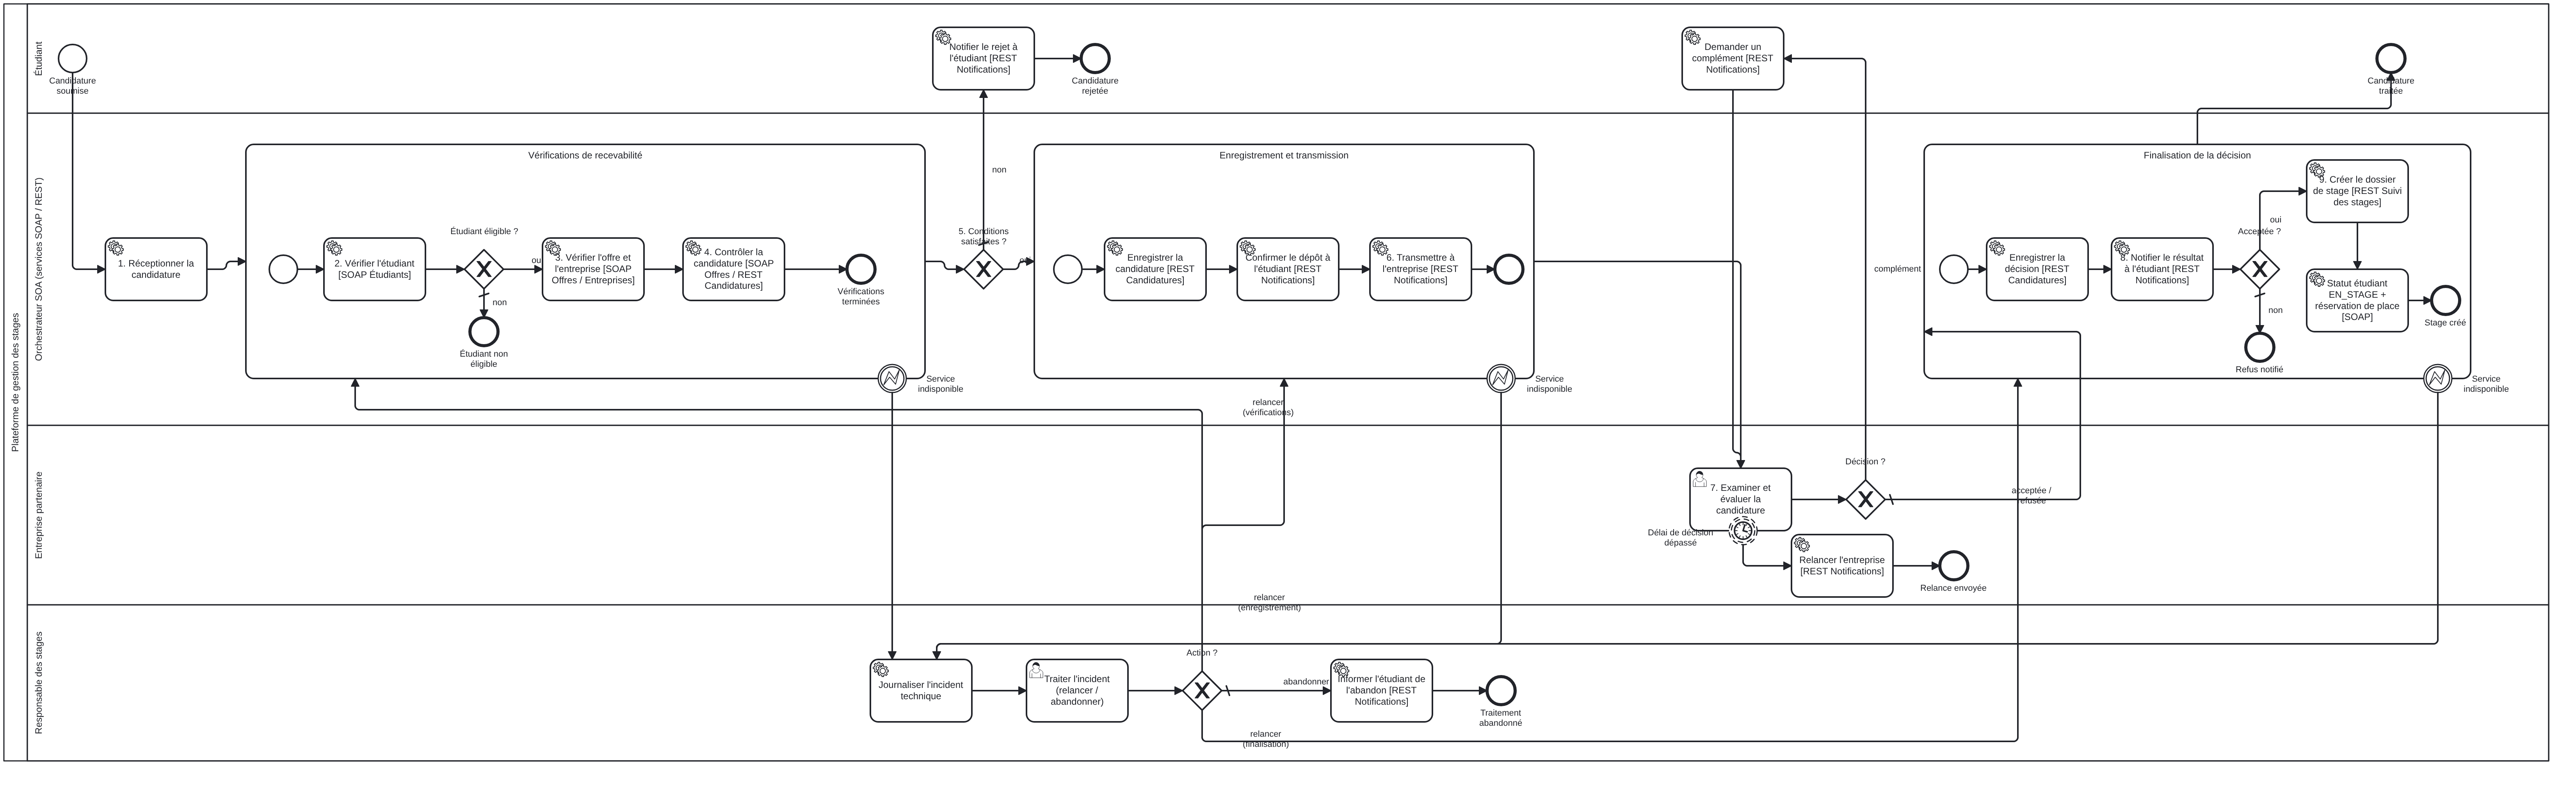
\includegraphics[width=\textheight]{figures/processus-bpmn.png}
\caption{Diagramme BPMN du processus de traitement d'une candidature (rendu bpmn-js du fichier exécuté)}\label{fig:bpmn}
\end{sidewaysfigure}

\section{Structure du processus}
Le pool « Plateforme de gestion des stages » comporte quatre couloirs : \emph{Étudiant}, \emph{Orchestrateur SOA},
\emph{Entreprise partenaire} et \emph{Responsable des stages}. Les étapes de l'orchestrateur sont regroupées en
trois \textbf{sous-processus} qui délimitent les zones de reprise en cas d'erreur.

\begin{table}[htbp]
\centering\small
\caption{Correspondance entre les étapes du sujet et le modèle BPMN}\label{tab:etapes}
\begin{tabularx}{\textwidth}{@{}lYY@{}}
\toprule
\textbf{Étape du sujet} & \textbf{Éléments BPMN} & \textbf{Service appelé} \\
\midrule
1. Réception & Événement de début « Candidature soumise » ; tâche « Réceptionner » (contrôle de forme, initialisation) & API \code{POST /processus/candidatures} \\
2. Vérification de l'étudiant & Tâche « Vérifier l'étudiant » ; passerelle « Étudiant éligible ? » & SOAP Étudiants : \code{verifierEtudiant}, \code{consulterEtudiant} \\
3. Vérification de l'offre & Tâche « Vérifier l'offre et l'entreprise » & SOAP Offres : \code{consulterOffre}, \code{verifierCompatibilite} ; SOAP Entreprises : \code{verifierEntreprise}, \code{consulterEntreprise} \\
4. Contrôle de la candidature & Tâche « Contrôler la candidature » & SOAP Offres : \code{verifierDisponibilite} ; REST : \code{GET /candidatures} (doublon) \\
5. Passerelle de décision & Passerelle exclusive « Conditions satisfaites ? » : rejet notifié \emph{ou} enregistrement & REST : \code{POST /notifications} \emph{ou} \code{POST /candidatures} \\
6. Transmission à l'entreprise & Sous-processus « Enregistrement et transmission » : confirmation à l'étudiant, notification de l'entreprise & REST Notifications \\
7. Décision de l'entreprise & Tâche humaine « Examiner et évaluer la candidature » : prise en charge (statut « en cours d'évaluation »), puis passerelle « Décision ? » (accepter, refuser, demander un complément) & API \code{…/prise-en-charge} puis \code{…/decision} ; REST \code{PATCH /candidatures/\{id\}/statut} \\
8. Notification du résultat & Tâche « Notifier le résultat » (gabarit ACCEPTATION ou REFUS) & REST Notifications \\
9. Mise à jour du suivi & Passerelle « Acceptée ? » ; « Créer le dossier de stage » ; « Statut EN\_STAGE + réservation de place » & REST : \code{POST /stages} ; SOAP : \code{changerStatutEtudiant}, \code{reserverPlace} \\
\bottomrule
\end{tabularx}
\end{table}

\section{Passerelles et conditions}
\begin{table}[htbp]
\centering\small
\caption{Passerelles exclusives et expressions de condition}
\begin{tabularx}{\textwidth}{@{}lYl@{}}
\toprule
\textbf{Passerelle} & \textbf{Branches (condition JUEL)} & \textbf{Défaut} \\
\midrule
Étudiant éligible ? & oui : \code{\$\{etudiantEligible\}} & fin « Étudiant non éligible » \\
Conditions satisfaites ? & oui : \code{\$\{recevable\}} → enregistrement & notification du rejet \\
Décision ? & complément : \code{\$\{decision == 'COMPLEMENT'\}} → notification puis retour à l'évaluation & finalisation \\
Acceptée ? & oui : \code{\$\{decision == 'ACCEPTEE'\}} → création du stage & fin « Refus notifié » \\
Action ? (incident) & relancer : \code{\$\{actionIncident == 'RELANCER' \&\& etapeCourante == '…'\}} (une branche par sous-processus) & abandon notifié \\
\bottomrule
\end{tabularx}
\end{table}

La variable \code{recevable} n'est vraie que si l'étudiant est actif, l'offre active, l'entreprise référencée, la
filière et le niveau compatibles, la date limite non dépassée, une place disponible, aucune candidature non annulée
n'existe pour le même couple étudiant/offre, et l'étudiant a moins de 5 candidatures en cours. Tous les motifs de refus sont accumulés dans \code{motifRejet} et repris
dans la notification adressée à l'étudiant.

\section{Gestion des erreurs et des indisponibilités}\label{sec:erreurs}
La gestion des erreurs est organisée en quatre niveaux.

\paragraph{1. Reprise automatique.} Tout appel inter-services passe par \code{Resilience.avecReprise} :
3 tentatives avec un délai exponentiel (400~ms, 800~ms), délais de connexion et de réponse bornés à 5~s.
Seules les erreurs \emph{techniques} sont rejouées (connexion impossible, délai dépassé, HTTP 5xx) ; une erreur
\emph{fonctionnelle} (HTTP 4xx, SOAP Fault métier) est propagée immédiatement.

\paragraph{2. Erreur BPMN et événement de bordure.} Si le service reste indisponible, le délégué lève
\code{BpmnError("ERREUR\_TECHNIQUE")} après avoir renseigné \code{serviceEnErreur}, \code{messageErreur} et
\code{activiteEnErreur}. Chacun des trois sous-processus porte un \textbf{événement d'erreur de bordure} « Service
indisponible » qui interrompt le sous-processus et dirige le flux vers « Journaliser l'incident ».

\paragraph{3. Traitement humain de l'incident.} La tâche « Traiter l'incident » est attribuée au responsable des
stages, qui choisit de \textbf{relancer} l'étape — le flux revient au début du sous-processus en erreur, identifié par
la variable \code{etapeCourante} positionnée par un écouteur d'exécution — ou d'\textbf{abandonner}, auquel cas
l'étudiant est informé et l'instance se termine par l'événement « Traitement abandonné ».

\paragraph{4. Notifications non bloquantes.} Une notification non envoyée ne justifie pas de bloquer un étudiant :
après les reprises, l'échec est consigné dans la variable \code{incidents} et le processus continue.

\begin{lstlisting}[language=Java, caption={Conversion d'une indisponibilité en erreur BPMN (\code{AbstractServiceDelegate})}]
@Override
public final void execute(DelegateExecution execution) {
    try {
        executer(execution);
    } catch (ServiceIndisponibleException e) {
        String msg = "Service « " + e.getService() + " » indisponible : " + e.getMessage();
        execution.setVariable("serviceEnErreur", e.getService());
        execution.setVariable("messageErreur", msg);
        execution.setVariable("activiteEnErreur", execution.getCurrentActivityId());
        throw new BpmnError(ERREUR_TECHNIQUE, msg);   // intercepté par l'événement de bordure
    }
}
\end{lstlisting}

\paragraph{Idempotence des reprises.} Relancer un sous-processus ne doit pas dupliquer les effets déjà produits :
l'enregistrement de la candidature est ignoré si \code{candidatureId} est déjà connu, la création du stage récupère le
stage existant en cas de réponse \code{409}, et la réservation de place est mémorisée par \code{placeReservee}.

\paragraph{Démonstration.} Le simulateur de pannes (\code{POST /api/admin/pannes} ou écran « Supervision ») rend
n'importe lequel des six services indisponible (HTTP~503) ; les scénarios PT-04 à PT-06 du chapitre~\ref{chap:tests}
vérifient automatiquement ces comportements.

\section{Autres mécanismes}
\begin{description}[style=nextline]
  \item[Minuteur de relance] Un événement minuteur de bordure \textbf{non interrompant} est attaché à « Évaluer la
        candidature ». Passé le délai (\code{P3D} par défaut, paramétrable), l'entreprise est relancée par une
        notification \code{RELANCE\_DECISION} sans que la tâche d'évaluation soit annulée.
  \item[Prise en charge] La candidature reste \code{DEPOSEE} — donc annulable par l'étudiant — tant que l'entreprise
        n'a pas ouvert le dossier. Le bouton « Examiner » attribue la tâche à l'entreprise (\emph{claim}) et fait passer la
        candidature \code{EN\_COURS\_EVALUATION} ; une décision rendue directement déclenche cette prise en charge.
  \item[Demande de complément] La branche « complément » de la passerelle « Décision ? » notifie l'étudiant puis revient
        à la tâche d'évaluation ; l'étudiant complète son dossier par \code{PATCH /candidatures/\{id\}}.
  \item[Annulation] Lorsqu'un étudiant annule sa candidature, le service Candidatures publie un événement
        « candidature annulée » ; l'orchestrateur, abonné, interrompt l'instance correspondante (statut \code{INTERROMPU}).
  \item[Cohérence] Une décision ne peut pas contourner le processus : un \code{PATCH} manuel vers \code{ACCEPTEE} ou
        \code{REFUSEE} sur une candidature orchestrée est refusé (\code{409 DECISION\_VIA\_PROCESSUS}).
  \item[Traçabilité] L'historique du moteur est exposé par \code{GET /processus/instances/\{id\}} : activités
        traversées avec horodatage et durée, activités actives, variables, raison d'arrêt. L'interface superpose ces
        informations au diagramme (figure~\ref{fig:ui-instance}).
\end{description}

\section{Reproduction dans Bonita Studio}\label{sec:bonita}
Le guide \code{docs/bonita/GUIDE\_BONITA.md} détaille la reproduction du processus dans Bonita :
\begin{enumerate}
  \item importer \code{docs/bonita/traitement-candidature-bonita.bpmn} (\emph{Fichier › Importer › BPMN 2.0}), variante
        préparée pour Bonita : flux à plat (Bonita ne gère pas les sous-processus embarqués), un événement d'erreur de
        bordure sur chaque tâche critique, aucune extension propriétaire, noms de tâches courts adaptés à la taille fixe
        des tâches de Bonita. L'import a été vérifié dans Bonita Studio ;
  \item déclarer les variables du processus (tableau du guide) ;
  \item associer à chaque tâche de service un connecteur \emph{Web Service SOAP} ou \emph{REST} (même opérations
        qu'au tableau~\ref{tab:etapes}, compte \code{systeme}) ;
  \item configurer \emph{Lever un événement d'erreur} en cas d'échec des connecteurs critiques, et \emph{Ignorer
        l'erreur} pour les notifications ;
  \item définir les acteurs \emph{entreprise} et \emph{responsable} ainsi que le minuteur non interrompant.
\end{enumerate}

\chapter{Règles de gestion}\label{chap:regles}

Les règles ci-dessous sont implémentées dans les services indiqués ; la colonne « Test » renvoie aux scénarios
automatisés du chapitre~\ref{chap:tests} qui les vérifient.

\begin{longtable}{@{}lp{8.3cm}>{\raggedright\arraybackslash}p{2.6cm}l@{}}
\caption{Règles de gestion}\label{tab:regles}\\
\toprule
\textbf{N°} & \textbf{Règle} & \textbf{Service} & \textbf{Test} \\
\midrule
\endfirsthead
\toprule
\textbf{N°} & \textbf{Règle} & \textbf{Service} & \textbf{Test} \\
\midrule
\endhead
\bottomrule
\endfoot
\multicolumn{4}{@{}l}{\textit{Étudiants}}\\
RG-01 & Le matricule est unique et respecte le format \code{[A-Z]\{1,3\}[0-9]\{4,10\}}. & Étudiants & ST-04, ST-05 \\
RG-02 & L'adresse e-mail d'un étudiant est unique (insensible à la casse). & Étudiants & — \\
RG-03 & Un étudiant créé sans statut est \code{ACTIF}. & Étudiants & ST-03 \\
RG-04 & Seul un étudiant \code{ACTIF} est éligible aux candidatures (un étudiant suspendu, en stage ou diplômé ne l'est pas). & Étudiants, BPMN & ST-07, PT-02 \\
RG-05 & Un étudiant en stage ne peut pas être supprimé. & Étudiants & — \\
RG-06 & Un étudiant ne consulte que sa propre fiche ; dans « Mon profil », il ne modifie que ses coordonnées (e-mail, téléphone, adresse) et ses compétences, jamais son identité, sa filière, son niveau ni son statut. & Étudiants & ST-06, ST-14 \\
RG-32 & Une entreprise ne voit pas les coordonnées personnelles d'un candidat (téléphone et e-mail masqués, adresse non transmise). & Étudiants & ST-12 \\
\multicolumn{4}{@{}l}{\textit{Entreprises et offres}}\\
RG-07 & La raison sociale d'une entreprise est unique ; la date de référencement est fixée à l'activation du référencement. & Entreprises & ST-08 \\
RG-08 & Une entreprise ayant des offres actives ne peut pas être supprimée. & Entreprises & ST-08 \\
RG-09 & Seule une entreprise référencée peut publier une offre. & Offres & ST-09 \\
RG-10 & Une entreprise ne gère que ses propres offres ; elle ne consulte et ne modifie que son profil (coordonnées et contact), sans changer sa raison sociale, son secteur ni son référencement. & Offres, Entreprises & ST-09, ST-14 \\
RG-11 & À la création, la date limite est future, la durée comprise entre 1 et 12 mois, le nombre de places positif ; l'offre est \code{ACTIVE} et toutes ses places sont disponibles. & Offres & ST-09 \\
RG-12 & Le nombre de places d'une offre ne peut descendre sous le nombre de places déjà attribuées. & Offres & — \\
RG-13 & Une offre dont des stagiaires ont été retenus ne peut être supprimée (seulement clôturée). & Offres & — \\
RG-14 & Une offre est disponible si elle est active, que sa date limite n'est pas dépassée et qu'il reste au moins une place. & Offres & ST-11 \\
RG-15 & Chaque offre a un type de stage qui fixe les niveaux autorisés : observation (initiation) pour les INE1, ouvrier / PFA pour les INE1 et INE2, PFE pour les INE3. Compatibilité : la filière de l'étudiant doit être ciblée (liste vide = toutes), son niveau doit être autorisé par le type de l'offre et la date limite non dépassée ; le score de compétences est indicatif. Une candidature incompatible est rejetée avec un motif explicite. & Offres, BPMN & ST-10, PT-11 \\
RG-33 & Un étudiant ne voit que les offres dont le type de stage est ouvert à son niveau (filtrage côté serveur). & Offres & ST-13 \\
RG-16 & L'acceptation d'une candidature réserve une place ; à zéro place, l'offre passe à \code{POURVUE}. La réservation ne peut pas rendre le compteur négatif. & Offres, BPMN & PT-01 \\
\multicolumn{4}{@{}l}{\textit{Candidatures}}\\
RG-17 & Un étudiant ne peut avoir qu'une candidature non annulée par offre. & Candidatures, BPMN & RT-02, PT-02 \\
RG-18 & Une candidature n'est enregistrée que si toutes les vérifications du processus sont satisfaites ; sinon l'étudiant reçoit un rejet motivé. & BPMN & PT-02 \\
RG-19 & Les transitions de statut suivent l'automate de la figure~\ref{fig:automate} ; tout changement est historisé (auteur, date, motif). & Candidatures & RT-03 \\
RG-20 & Une candidature ne peut être annulée que tant qu'elle est \code{DEPOSEE} (l'entreprise ne l'a pas encore prise en charge), par l'étudiant concerné ou le responsable ; l'annulation interrompt le processus. & Candidatures, BPMN & RT-03, PT-07, PT-09 \\
RG-31 & Un étudiant ne peut avoir plus de 5 candidatures en cours (déposées ou en évaluation) ; au-delà, la candidature est rejetée. & Candidatures, BPMN & PT-10 \\
RG-21 & La décision sur une candidature orchestrée passe obligatoirement par la tâche « Évaluer » du processus. & Candidatures & — \\
RG-22 & Seule l'entreprise qui a publié l'offre (ou le responsable) peut rendre la décision. & Processus & PT-01 \\
RG-23 & Une demande de complément exige un commentaire, transmis à l'étudiant ; celui-ci peut alors compléter son dossier. & Processus & PT-03 \\
\multicolumn{4}{@{}l}{\textit{Notifications}}\\
RG-24 & L'étudiant est notifié par e-mail du dépôt, du rejet, d'une demande de complément, de la décision et d'un éventuel abandon ; l'entreprise de la réception et des relances. & Notifications, BPMN & PT-01, PT-03 \\
RG-25 & Sans décision après le délai fixé (3 jours par défaut), l'entreprise est relancée sans que l'évaluation soit annulée. & BPMN & PT-08 \\
RG-26 & Les étudiants actifs au profil compatible reçoivent un rappel unique par offre clôturant dans les 3 jours. & Notifications & — \\
RG-27 & Une notification non envoyée ne bloque jamais le processus ; l'incident est consigné. & BPMN & PT-06 \\
\multicolumn{4}{@{}l}{\textit{Stages}}\\
RG-28 & Un seul stage par candidature acceptée ; la date de fin est postérieure à la date de début ; le stage est \code{PLANIFIE} si son début est futur, \code{EN\_COURS} sinon. & Stages & RT-05 \\
RG-29 & Les comptes rendus ne sont acceptés que pour un stage planifié ou en cours ; la note d'une évaluation est comprise entre 0 et 20 et il n'y a qu'une évaluation finale. & Stages & RT-05 \\
RG-30 & L'évaluation finale clôture le stage ; à la fin ou à l'interruption du stage, l'étudiant redevient \code{ACTIF}. & Stages & RT-05 \\
\end{longtable}

\chapter{Scénarios de test}\label{chap:tests}

\section{Stratégie}
Trois niveaux de tests complémentaires ont été mis en place :
\begin{enumerate}
  \item \textbf{Tests d'intégration automatisés} (JUnit 5, \code{PlateformeIT}) : la plateforme complète est démarrée
        sur des bases H2 en mémoire puis sollicitée par de \emph{vrais} appels SOAP (clients JAX-WS générés depuis le WSDL)
        et HTTP. Les tests couvrent les services un par un puis le processus de bout en bout, y compris les pannes.
        Ils s'exécutent à chaque \code{mvn package} et ont également été exécutés sur \textbf{PostgreSQL~16}.
  \item \textbf{Collection Postman} (\code{docs/postman}) : 39 requêtes enchaînées avec 45 assertions sur les codes
        et les contenus, authentifiées par clé d'API, exécutable dans le \emph{Collection Runner} ou avec Newman.
  \item \textbf{Requêtes SoapUI} (\code{docs/soap}) : enveloppes prêtes à l'emploi pour chaque type d'opération,
        accompagnées des réponses réellement obtenues.
\end{enumerate}

\section{Tests automatisés}
\begin{longtable}{@{}lp{7.2cm}p{5.2cm}c@{}}
\caption{Scénarios de test automatisés et résultats}\label{tab:tests}\\
\toprule
\textbf{ID} & \textbf{Scénario} & \textbf{Résultat attendu} & \textbf{Résultat} \\
\midrule
\endfirsthead
\toprule
\textbf{ID} & \textbf{Scénario} & \textbf{Résultat attendu} & \textbf{Résultat} \\
\midrule
\endhead
\bottomrule
\endfoot
\multicolumn{4}{@{}l}{\textit{Services SOAP}}\\
ST-01 & Récupérer les trois WSDL & Opérations présentes dans chaque contrat & \ok \\
ST-02 & Appel SOAP sans en-tête WS-Security & Fault \code{FailedAuthentication} & \ok \\
ST-03 & Ajouter, consulter, modifier, supprimer un étudiant & Statut \code{ACTIF} par défaut ; consultation après suppression : \code{RESSOURCE\_INTROUVABLE} & \ok \\
ST-04 & Ajouter un étudiant (matricule, e-mail et niveau invalides) & Fault \code{DONNEES\_INVALIDES} avec 3 détails & \ok \\
ST-05 & Ajouter un matricule existant & Fault \code{CONFLIT} & \ok \\
ST-06 & Un étudiant consulte une autre fiche / supprime sa fiche & Fault \code{ACCES\_REFUSE} & \ok \\
ST-07 & Vérifier un étudiant actif, suspendu, inexistant & éligible / non éligible / inexistant & \ok \\
ST-08 & CRUD entreprise ; offres d'une entreprise ; suppression avec offres actives & 2 offres ; \code{REGLE\_METIER} & \ok \\
ST-09 & Publier une offre : entreprise non référencée, autre entreprise, entreprise propriétaire & \code{REGLE\_METIER}, \code{ACCES\_REFUSE}, offre \code{ACTIVE} & \ok \\
ST-10 & Compatibilité AMOA/INE3, DATA/INE1 et offre expirée & compatible, score 50 \% ; incompatible, 2 motifs ; incompatible (date limite) & \ok \\
ST-11 & Disponibilité d'une offre expirée & date dépassée, non disponible & \ok \\
ST-12 & Fiche d'un candidat consultée par une entreprise puis par le responsable & téléphone et e-mail masqués, adresse absente ; fiche complète & \ok \\
\multicolumn{4}{@{}l}{\textit{Services REST}}\\
RT-01 & Requêtes sans identifiants, avec mauvais mot de passe, rôle étudiant sur \code{POST /stages} & 401, 401, 403 & \ok \\
RT-02 & Dépôt invalide, valide, en double, JSON mal formé & 400, 201 \code{DEPOSEE}, 409, 400 & \ok \\
RT-03 & Transition interdite, annulation par un tiers, passage en évaluation, annulation refusée, historique ; annulation d'une candidature déposée & 409, 403, 200, 422, 3 entrées ; \code{ANNULEE} puis 422 & \ok \\
RT-04 & Notification d'acceptation ; lecture par un autre étudiant ; type inconnu & 201 et message rendu ; 403 ; 400 & \ok \\
RT-05 & Stage : création, doublon, compte rendu, note 25, évaluation finale, historique & 201 \code{EN\_COURS}, 409, 201, 400, \code{TERMINE}, moyenne 16,5, étudiant \code{ACTIF} & \ok \\
RT-06 & Clé d'API valide, invalide, régénérée ; ancienne clé & 200 ; 401 \code{CLE\_API\_INVALIDE} ; 200 ; 401 (révoquée) & \ok \\
\multicolumn{4}{@{}l}{\textit{Processus BPMN}}\\
PT-01 & Scénario nominal : candidature puis acceptation par l'entreprise & Stage créé aux dates saisies, étudiant \code{EN\_STAGE}, offre \code{POURVUE}, 3 notifications ; tâche invisible pour une autre entreprise & \ok \\
PT-02 & Candidatures non recevables : étudiant suspendu, niveau insuffisant, date dépassée, entreprise non référencée, offre pourvue & 5 instances terminées par « Candidature rejetée » avec motif & \ok \\
PT-03 & Complément sans commentaire, complément, puis refus & 400 ; retour à l'évaluation ; \code{REFUSEE} ; notifications \code{DEMANDE\_COMPLEMENT} et \code{REFUS} & \ok \\
PT-04 & Service Candidatures en panne pendant les vérifications, puis relance & \code{INCIDENT\_TECHNIQUE} (étape \code{VERIFICATIONS}) puis \code{EN\_ATTENTE\_DECISION} & \ok \\
PT-05 & Service Stages en panne pendant la finalisation, puis abandon & \code{INCIDENT\_TECHNIQUE} (étape \code{FINALISATION}) puis \code{ABANDONNEE} & \ok \\
PT-06 & Service Notifications en panne pendant le dépôt & Processus poursuivi, incident consigné & \ok \\
PT-07 & Annulation d'une candidature déposée & Instance \code{INTERROMPU} & \ok \\
PT-08 & Délai de décision dépassé (2 s en test) & Relance de l'entreprise, évaluation toujours en attente & \ok \\
PT-09 & Prise en charge par l'entreprise puis tentative d'annulation & \code{DEPOSEE} → \code{EN\_COURS\_EVALUATION}, tâche attribuée, annulation refusée (422) & \ok \\
PT-10 & Sixième candidature en cours pour un même étudiant & Rejet motivé par le processus ; 422 sur l'API & \ok \\
\end{longtable}

\begin{lstlisting}[language=sh, caption={Exécution de la suite (extrait de la sortie Maven Surefire)}]
$ mvn test
Tests run: 12, Failures: 0, Errors: 0, Skipped: 0 -- in PlateformeIT$Soap
Tests run: 6,  Failures: 0, Errors: 0, Skipped: 0 -- in PlateformeIT$Rest
Tests run: 10, Failures: 0, Errors: 0, Skipped: 0 -- in PlateformeIT$Processus

$ mvn test -Ddb.url=jdbc:postgresql://localhost:5433/stages -Dbpmn.db.url=jdbc:postgresql://...
Tests run: 24, Failures: 0, Errors: 0, Skipped: 0
\end{lstlisting}

\begin{lstlisting}[language=Java, caption={Exemple de test : indisponibilité puis relance (PT-04)}]
@Test
@DisplayName("PT-04 Indisponibilité d'un service : incident, tâche du responsable, relance réussie")
void incidentRelance() {
    SimulateurPannes.definir("candidatures", true);
    JsonNode r;
    try {
        r = soumettre("E2026003", 4).json();
    } finally {
        SimulateurPannes.definir("candidatures", false);
    }
    assertEquals("INCIDENT_TECHNIQUE", r.get("statut").asText());
    assertEquals("VERIFICATIONS", r.get("variables").get("etapeCourante").asText());
    JsonNode apres = Http.post("/api/processus/taches/" + tache(r, "traiterIncident") + "/incident",
            ADMIN, ADMIN_PWD, Map.of("action", "RELANCER")).json();
    assertEquals("EN_ATTENTE_DECISION", apres.get("statut").asText());
}
\end{lstlisting}

\section{Collection Postman}
La collection est organisée en six dossiers (système, processus, candidatures, notifications, stages, pannes). Les
variables de collection (\code{tacheId}, \code{candidatureId}, \code{stageId}, \code{incidentId}) sont alimentées par
les scripts de test, ce qui permet d'enchaîner un scénario complet.

\begin{lstlisting}[language=sh, caption={Exécution de la collection avec Newman}]
$ newman run docs/postman/gestion-stages.postman_collection.json
|                requests |                 39 |                 0 |
|              assertions |                 45 |                 0 |
\end{lstlisting}

\section{Requêtes SoapUI}
Après import des trois WSDL dans SoapUI, les enveloppes de \code{docs/soap/} peuvent être collées telles quelles :

\begin{table}[H]
\centering\small
\caption{Requêtes SOAP fournies}
\begin{tabularx}{\textwidth}{@{}lYl@{}}
\toprule
\textbf{Fichier} & \textbf{Cas} & \textbf{Résultat obtenu} \\
\midrule
\code{01-etudiants-ajouterEtudiant} & Création d'une étudiante & fiche \code{ACTIF} \\
\code{02-etudiants-consulterEtudiant} & Consultation & fiche complète \\
\code{03-etudiants-verifierEtudiant} & Étudiante suspendue & \code{eligible=false} \\
\code{04-etudiants-ajouterEtudiant-invalide} & Données invalides & Fault, 3 détails \\
\code{05-entreprises-verifierEntreprise} & Entreprise non référencée & \code{referencee=false} \\
\code{06-entreprises-consulterOffresEntreprise} & Composition SOAP & 2 offres \\
\code{07-offres-creerOffre} & Publication d'une offre & offre \code{ACTIVE} \\
\code{08-offres-verifierDisponibilite} & Offre expirée & \code{disponible=false} \\
\code{09-offres-verifierCompatibilite} & Score de compétences & 50 \%, 2 manques \\
\code{10-sans-ws-security} & Sans authentification & \code{wsse:FailedAuthentication} \\
\bottomrule
\end{tabularx}
\end{table}

\chapter{Interface graphique (bonus)}\label{chap:interface}

\section{Principes}
L'interface est une application web monopage (HTML, CSS, JavaScript sans framework) servie par la plateforme. Elle
consomme \emph{directement} les services : un petit client SOAP en JavaScript (\code{soap.js}) construit les enveloppes
avec l'en-tête WS-Security et convertit les réponses XML, tandis que les services REST sont appelés en JSON. Le
diagramme BPMN est affiché avec \textbf{bpmn-js}, embarqué dans l'application, ce qui permet de suivre une instance
en direct. La charte reprend le bleu de l'INPT. Après connexion, le menu s'adapte au rôle :

\begin{table}[htbp]
\centering\small
\caption{Écrans par acteur}
\begin{tabularx}{\textwidth}{@{}lY@{}}
\toprule
\textbf{Acteur} & \textbf{Écrans} \\
\midrule
Étudiant & Offres ouvertes à son année d'études, avec type de stage (badge et filtre), score d'adéquation et motifs d'incompatibilité ; dépôt de candidature (déclenche le
  processus) ; suivi des candidatures (chronologie en 5 étapes), complément et annulation ; notifications ; « Mon stage » (progression,
  comptes rendus, évaluations) ; « Mon profil » (coordonnées et compétences modifiables) \\
Entreprise & Candidatures à évaluer (profil, compétences, lettre, CV) et formulaire de décision ; publication (choix
  du type de stage) et clôture d'offres (SOAP) ; candidatures reçues ; stagiaires, démarrage du stage et évaluations ; « Mon profil » (coordonnées et contact modifiables) \\
Responsable & Tableau de bord ; processus BPMN et instances (diagramme surligné, trace, variables) ; incidents
  (relancer, abandonner) ; gestion des étudiants et entreprises (SOAP) ; offres (avec leur type de stage), candidatures et stages ; supervision
  (pannes simulées, campagne de rappels) ; « Ma clé d'API » \\
\bottomrule
\end{tabularx}
\end{table}

\section{Parcours de l'étudiant}
\begin{figure}[H]
\centering
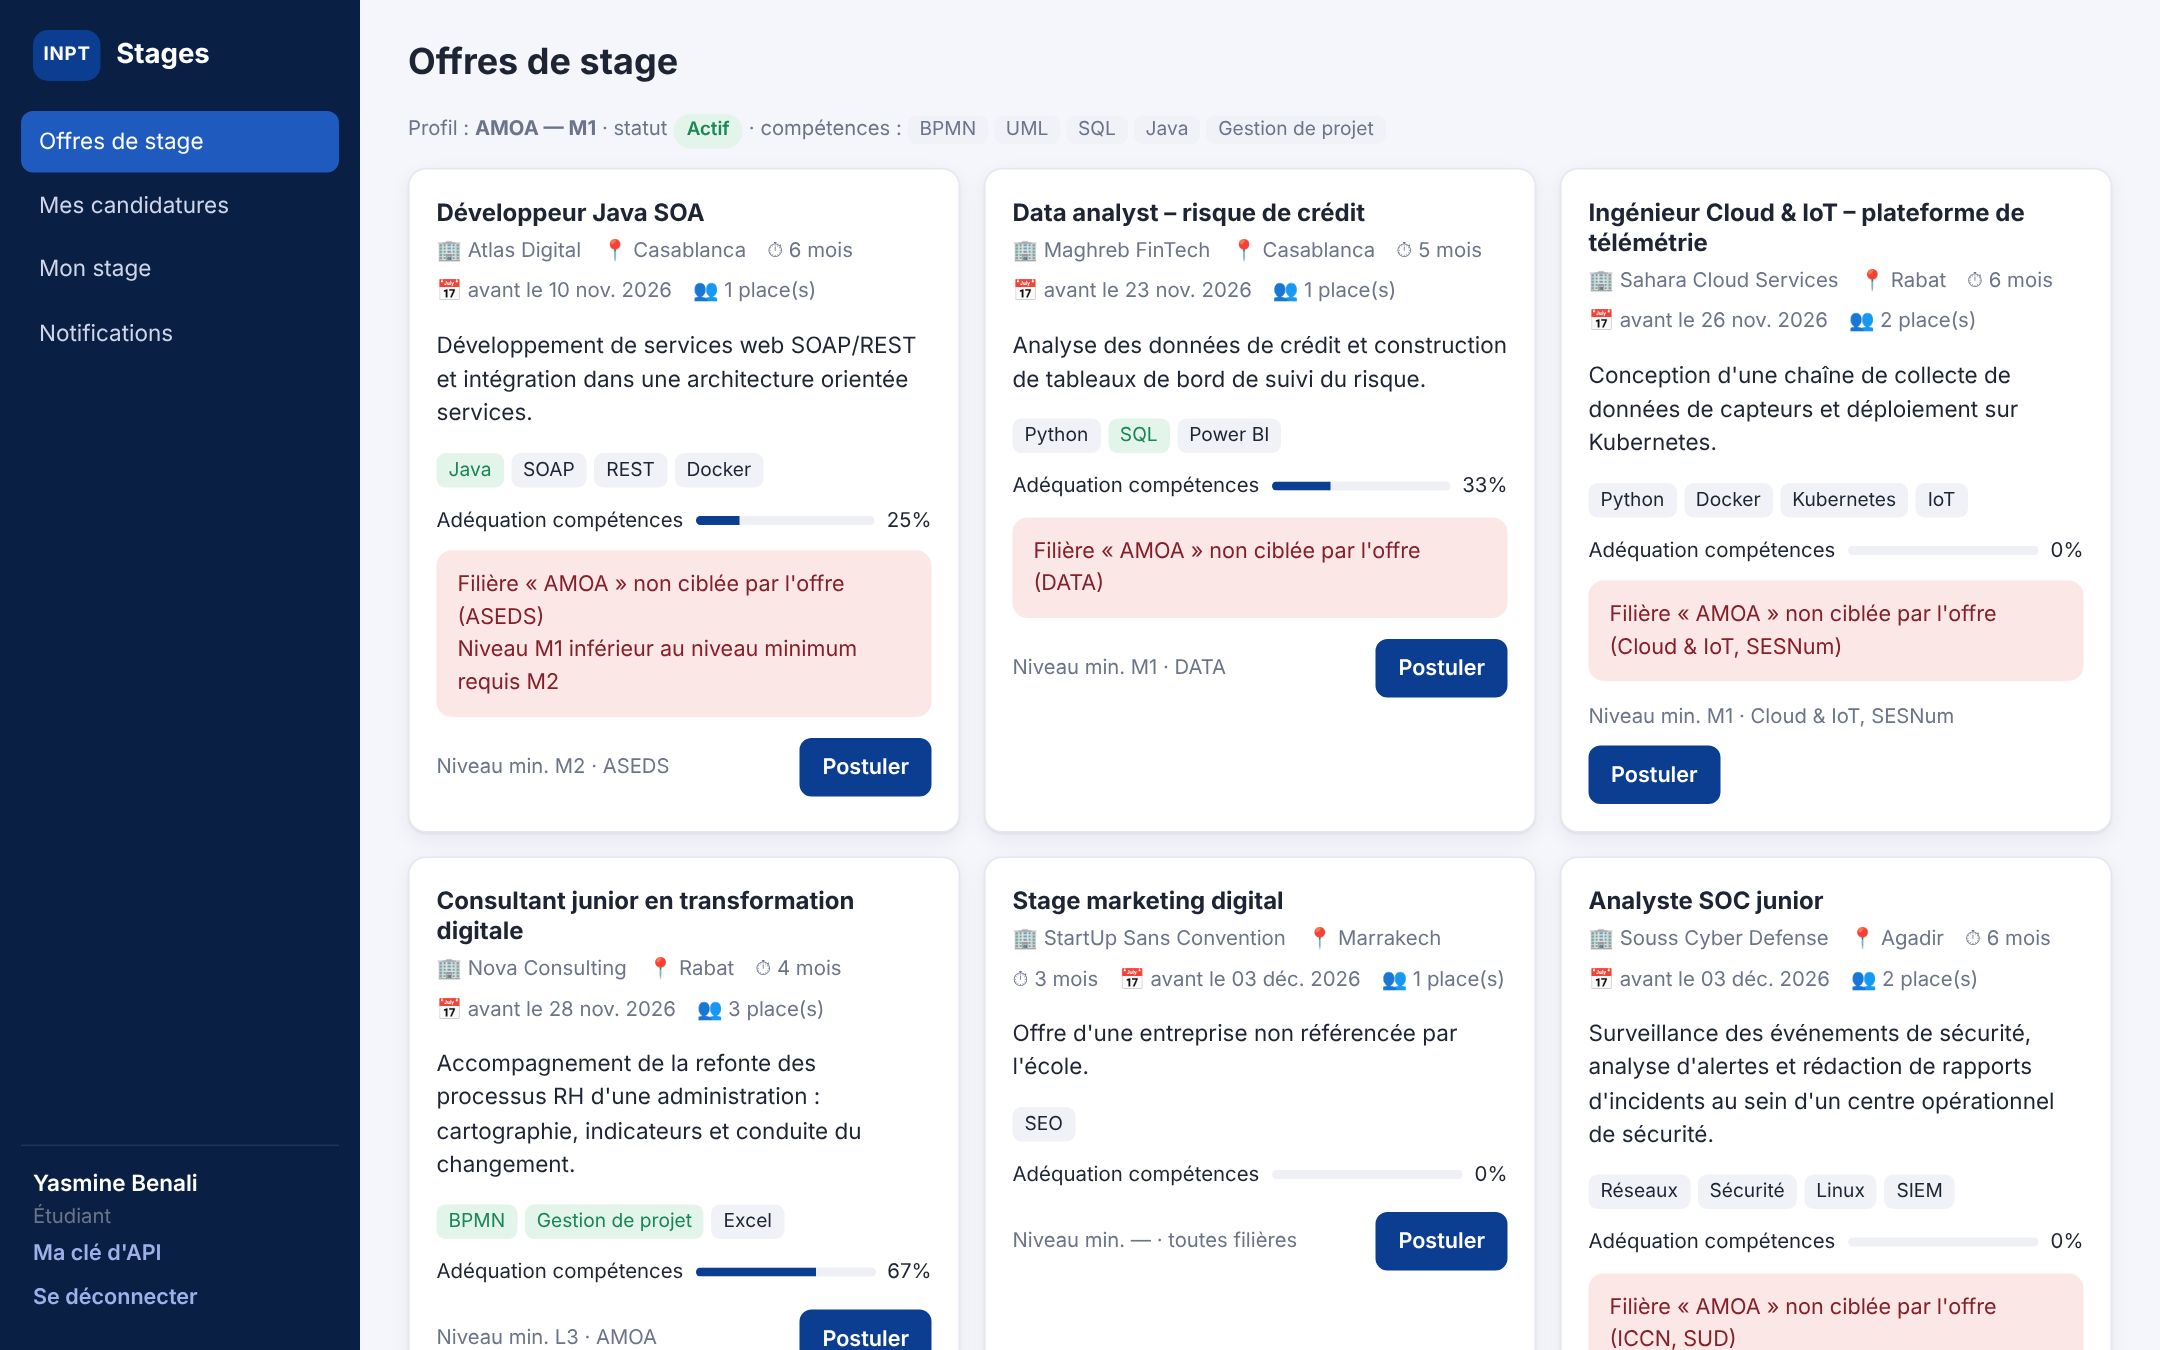
\includegraphics[width=0.92\textwidth]{figures/ui-etudiant-offres.png}
\caption{Offres de stage : score d'adéquation et motifs d'incompatibilité calculés par \code{verifierCompatibilite}}
\end{figure}

\begin{figure}[H]
\centering
\begin{minipage}{0.49\textwidth}\centering
  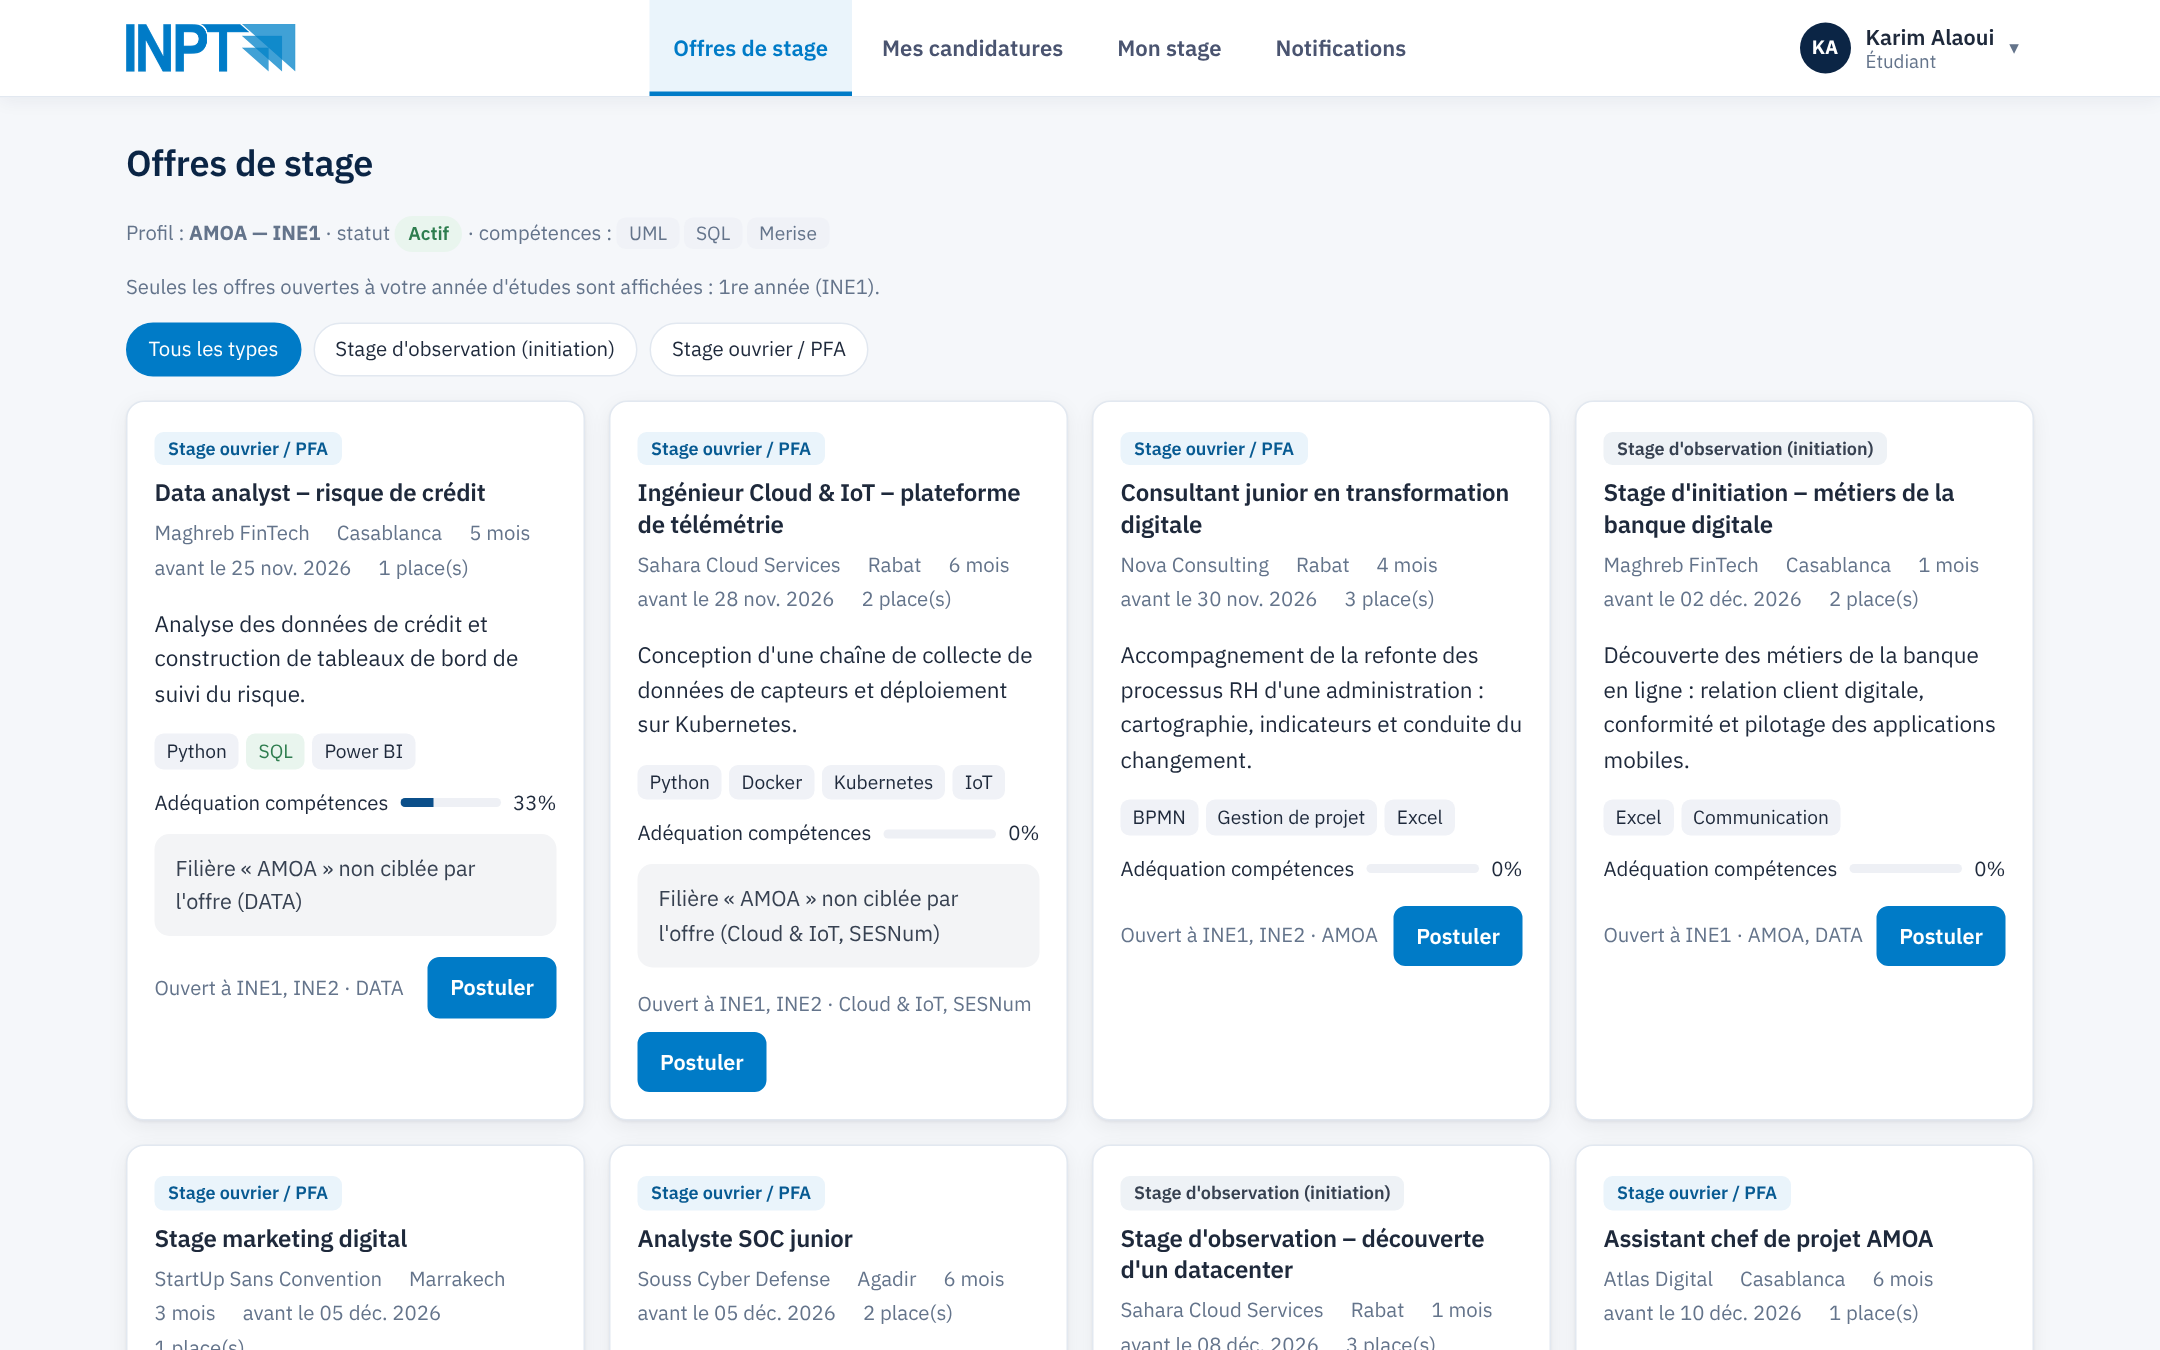
\includegraphics[width=\linewidth]{figures/ui-etudiant-offres-types.png}\\[-2pt]{\small (a) étudiant de 1re année : observation et ouvrier / PFA, filtre par type}
\end{minipage}\hfill
\begin{minipage}{0.49\textwidth}\centering
  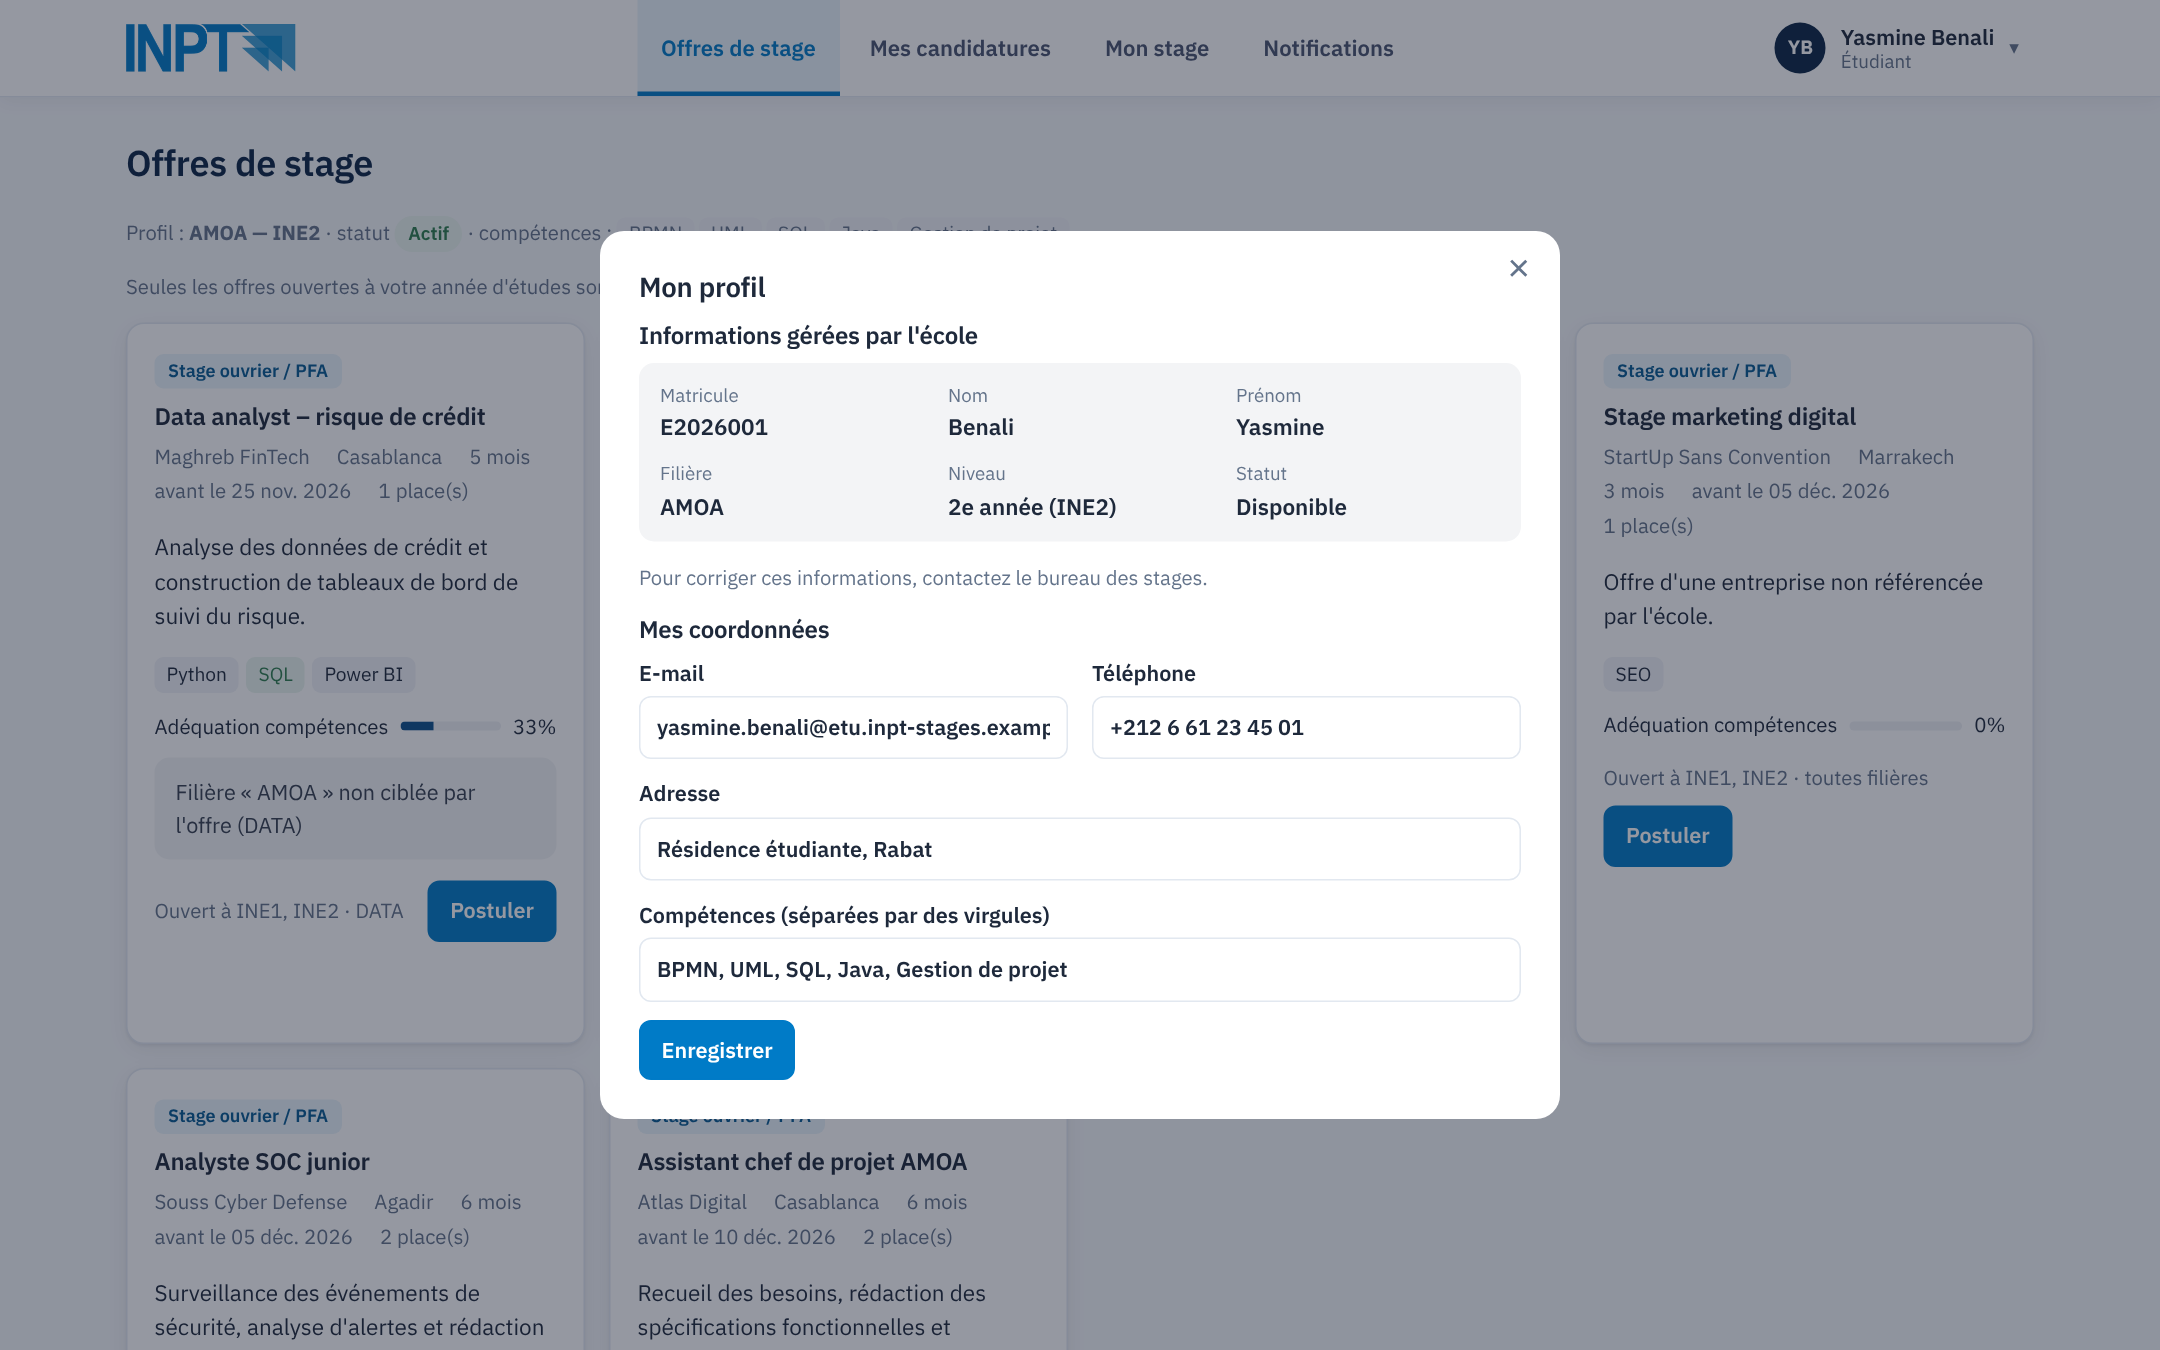
\includegraphics[width=\linewidth]{figures/ui-etudiant-profil.png}\\[-2pt]{\small (b) « Mon profil » : champs gérés par l'école en lecture seule}
\end{minipage}
\caption{Offres filtrées selon l'année d'études et profil de l'étudiant}
\end{figure}

\begin{figure}[H]
\centering
\begin{minipage}{0.49\textwidth}\centering
  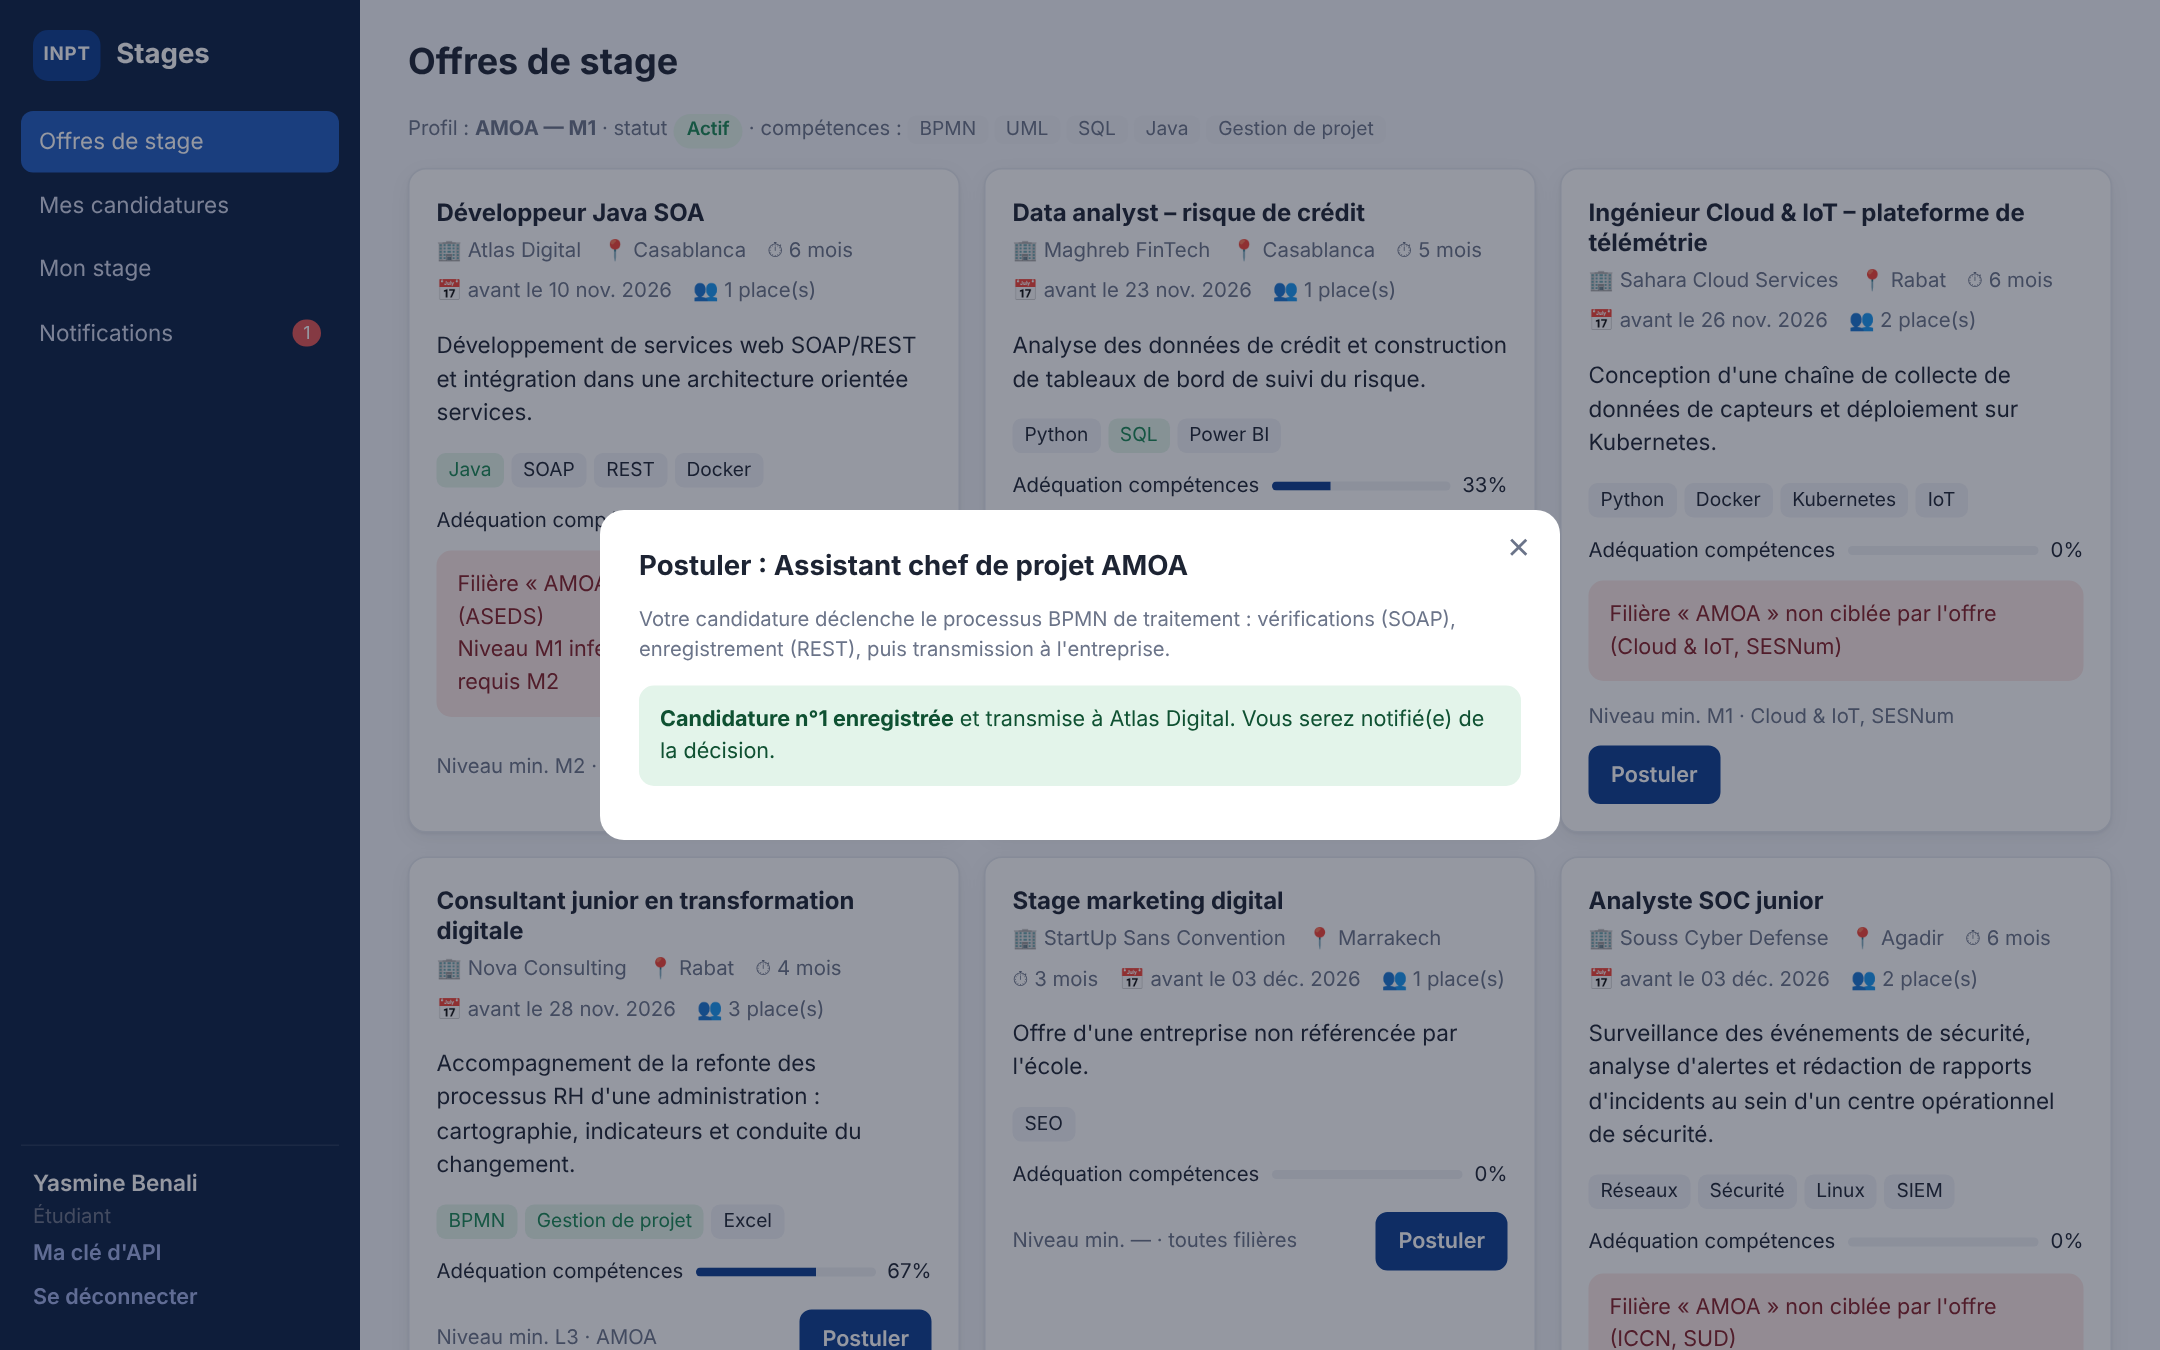
\includegraphics[width=\linewidth]{figures/ui-etudiant-postuler.png}\\[-2pt]{\small (a) candidature enregistrée}
\end{minipage}\hfill
\begin{minipage}{0.49\textwidth}\centering
  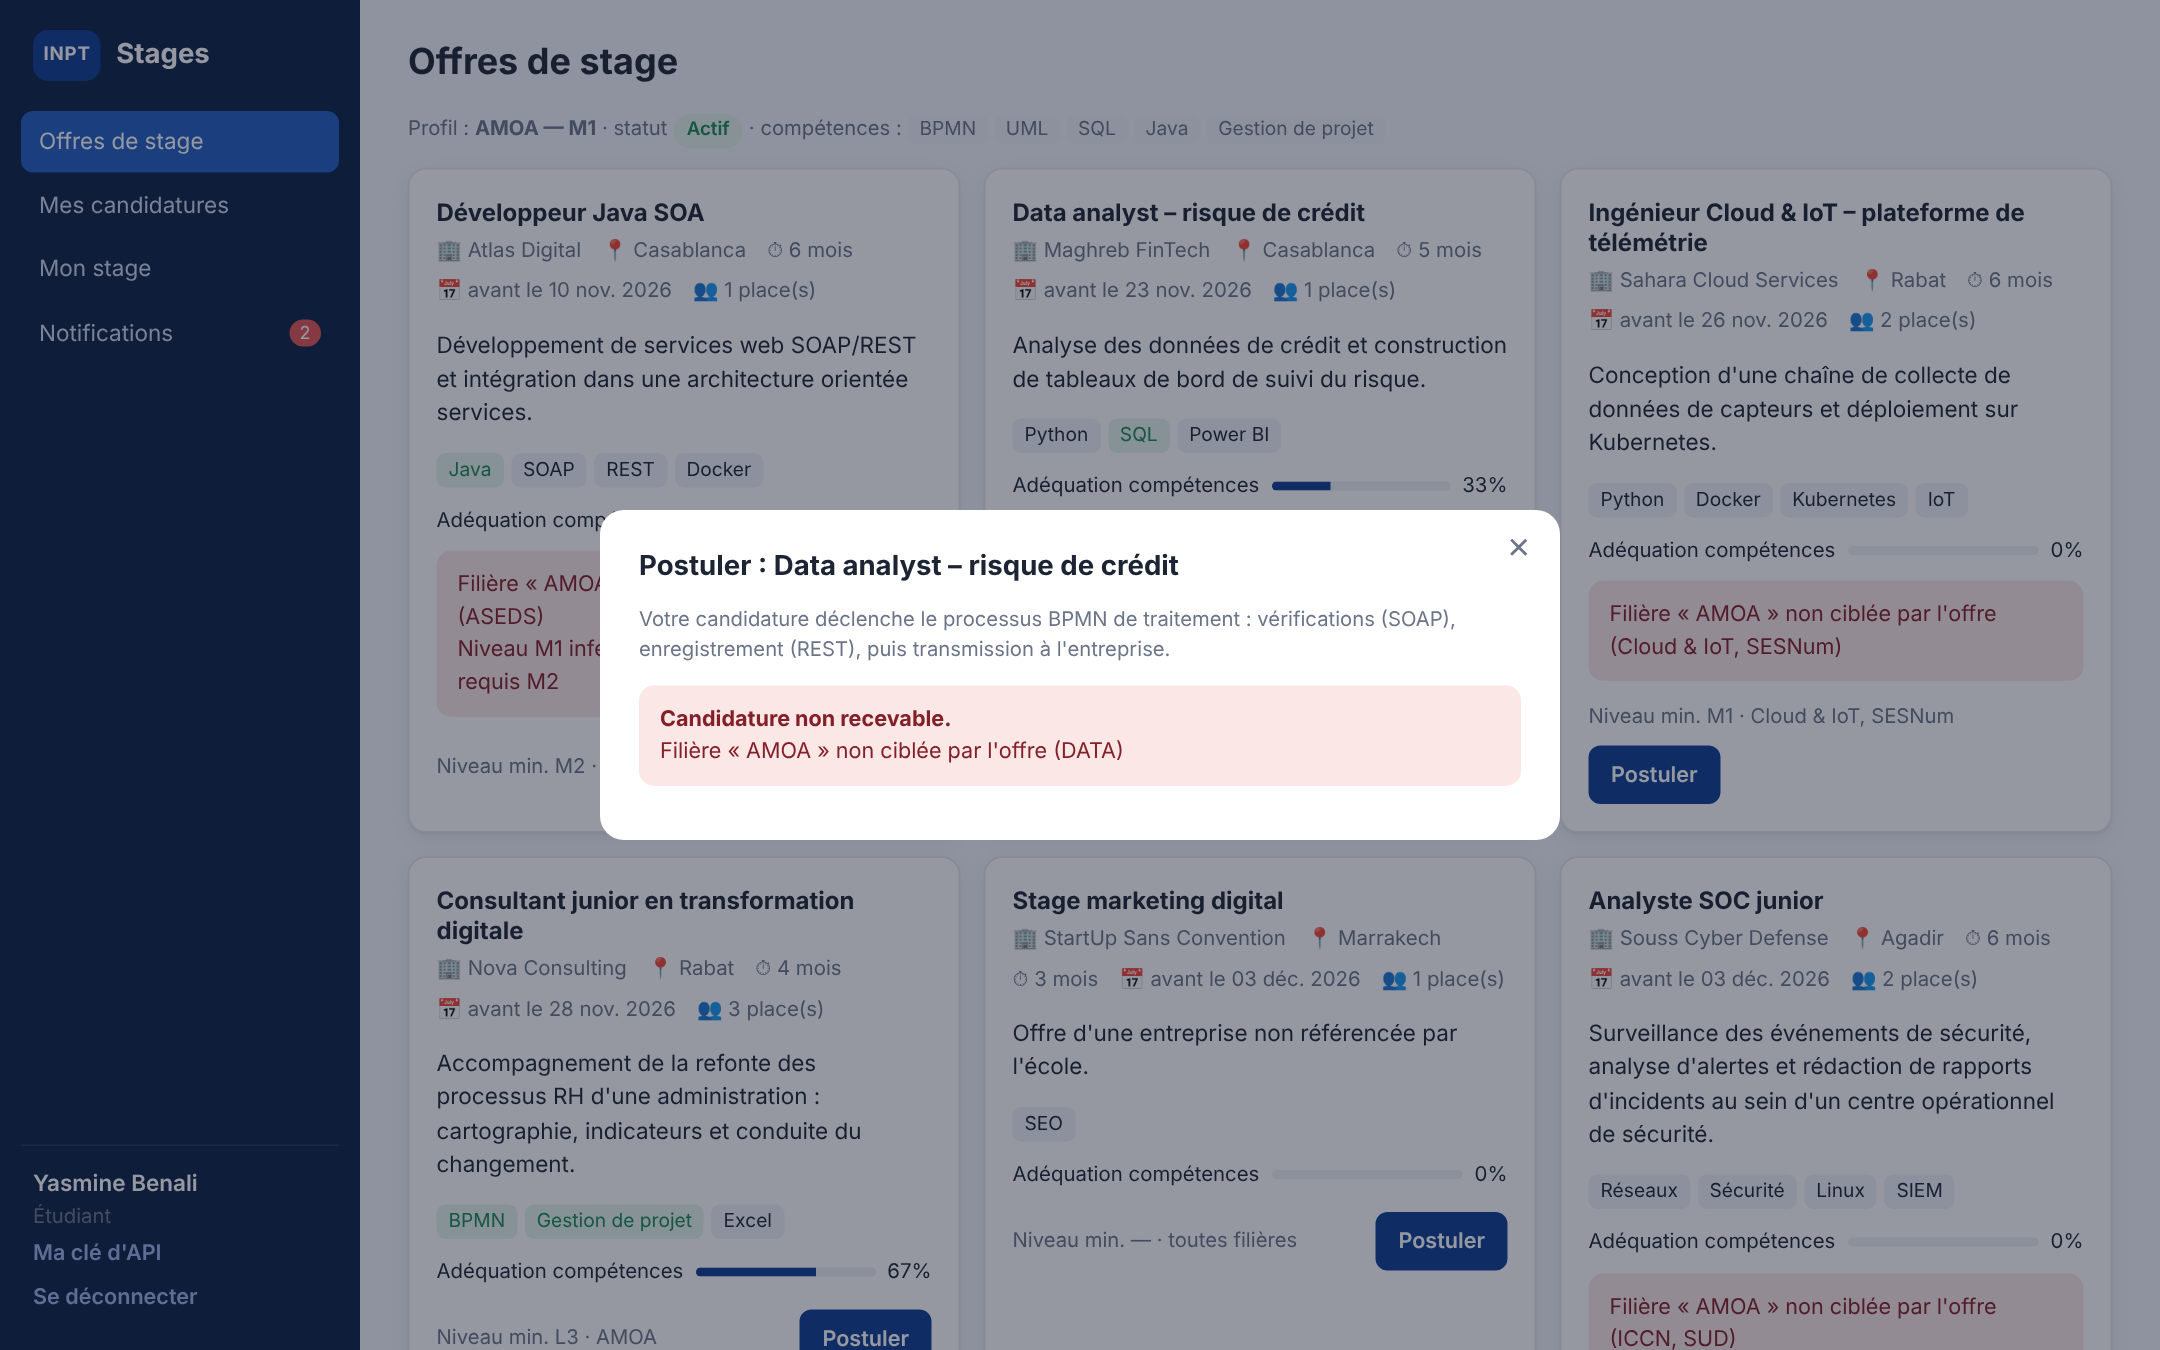
\includegraphics[width=\linewidth]{figures/ui-etudiant-rejet.png}\\[-2pt]{\small (b) rejet motivé par le processus}
\end{minipage}
\caption{Résultat d'une soumission de candidature}
\end{figure}

\begin{figure}[H]
\centering
\begin{minipage}{0.49\textwidth}\centering
  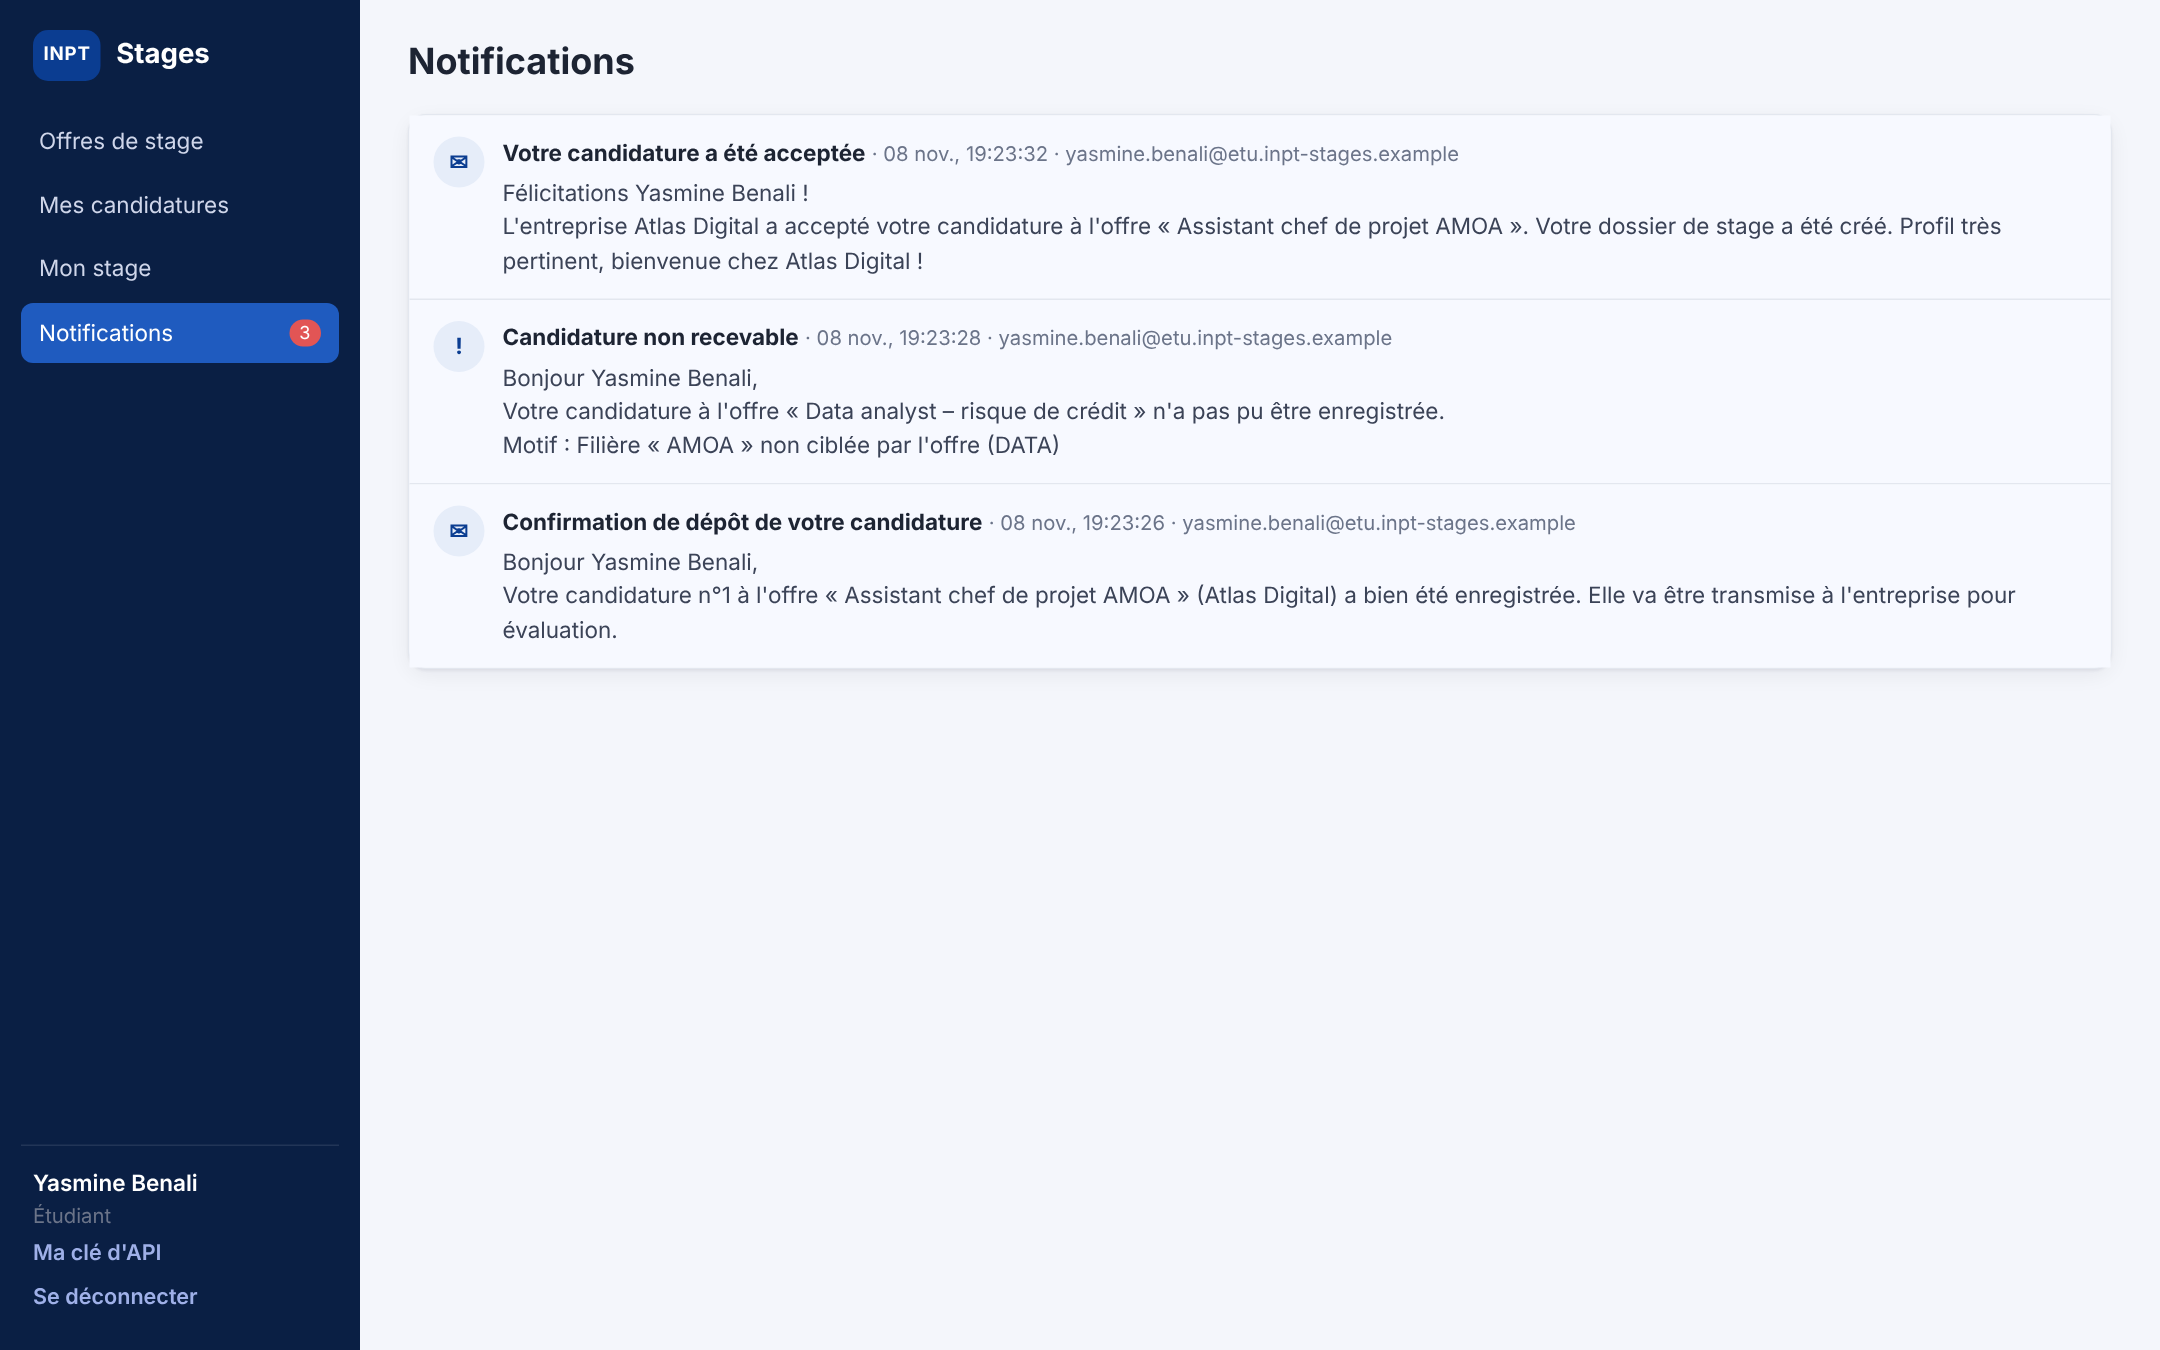
\includegraphics[width=\linewidth]{figures/ui-etudiant-notifications.png}\\[-2pt]{\small (a) notifications reçues}
\end{minipage}\hfill
\begin{minipage}{0.49\textwidth}\centering
  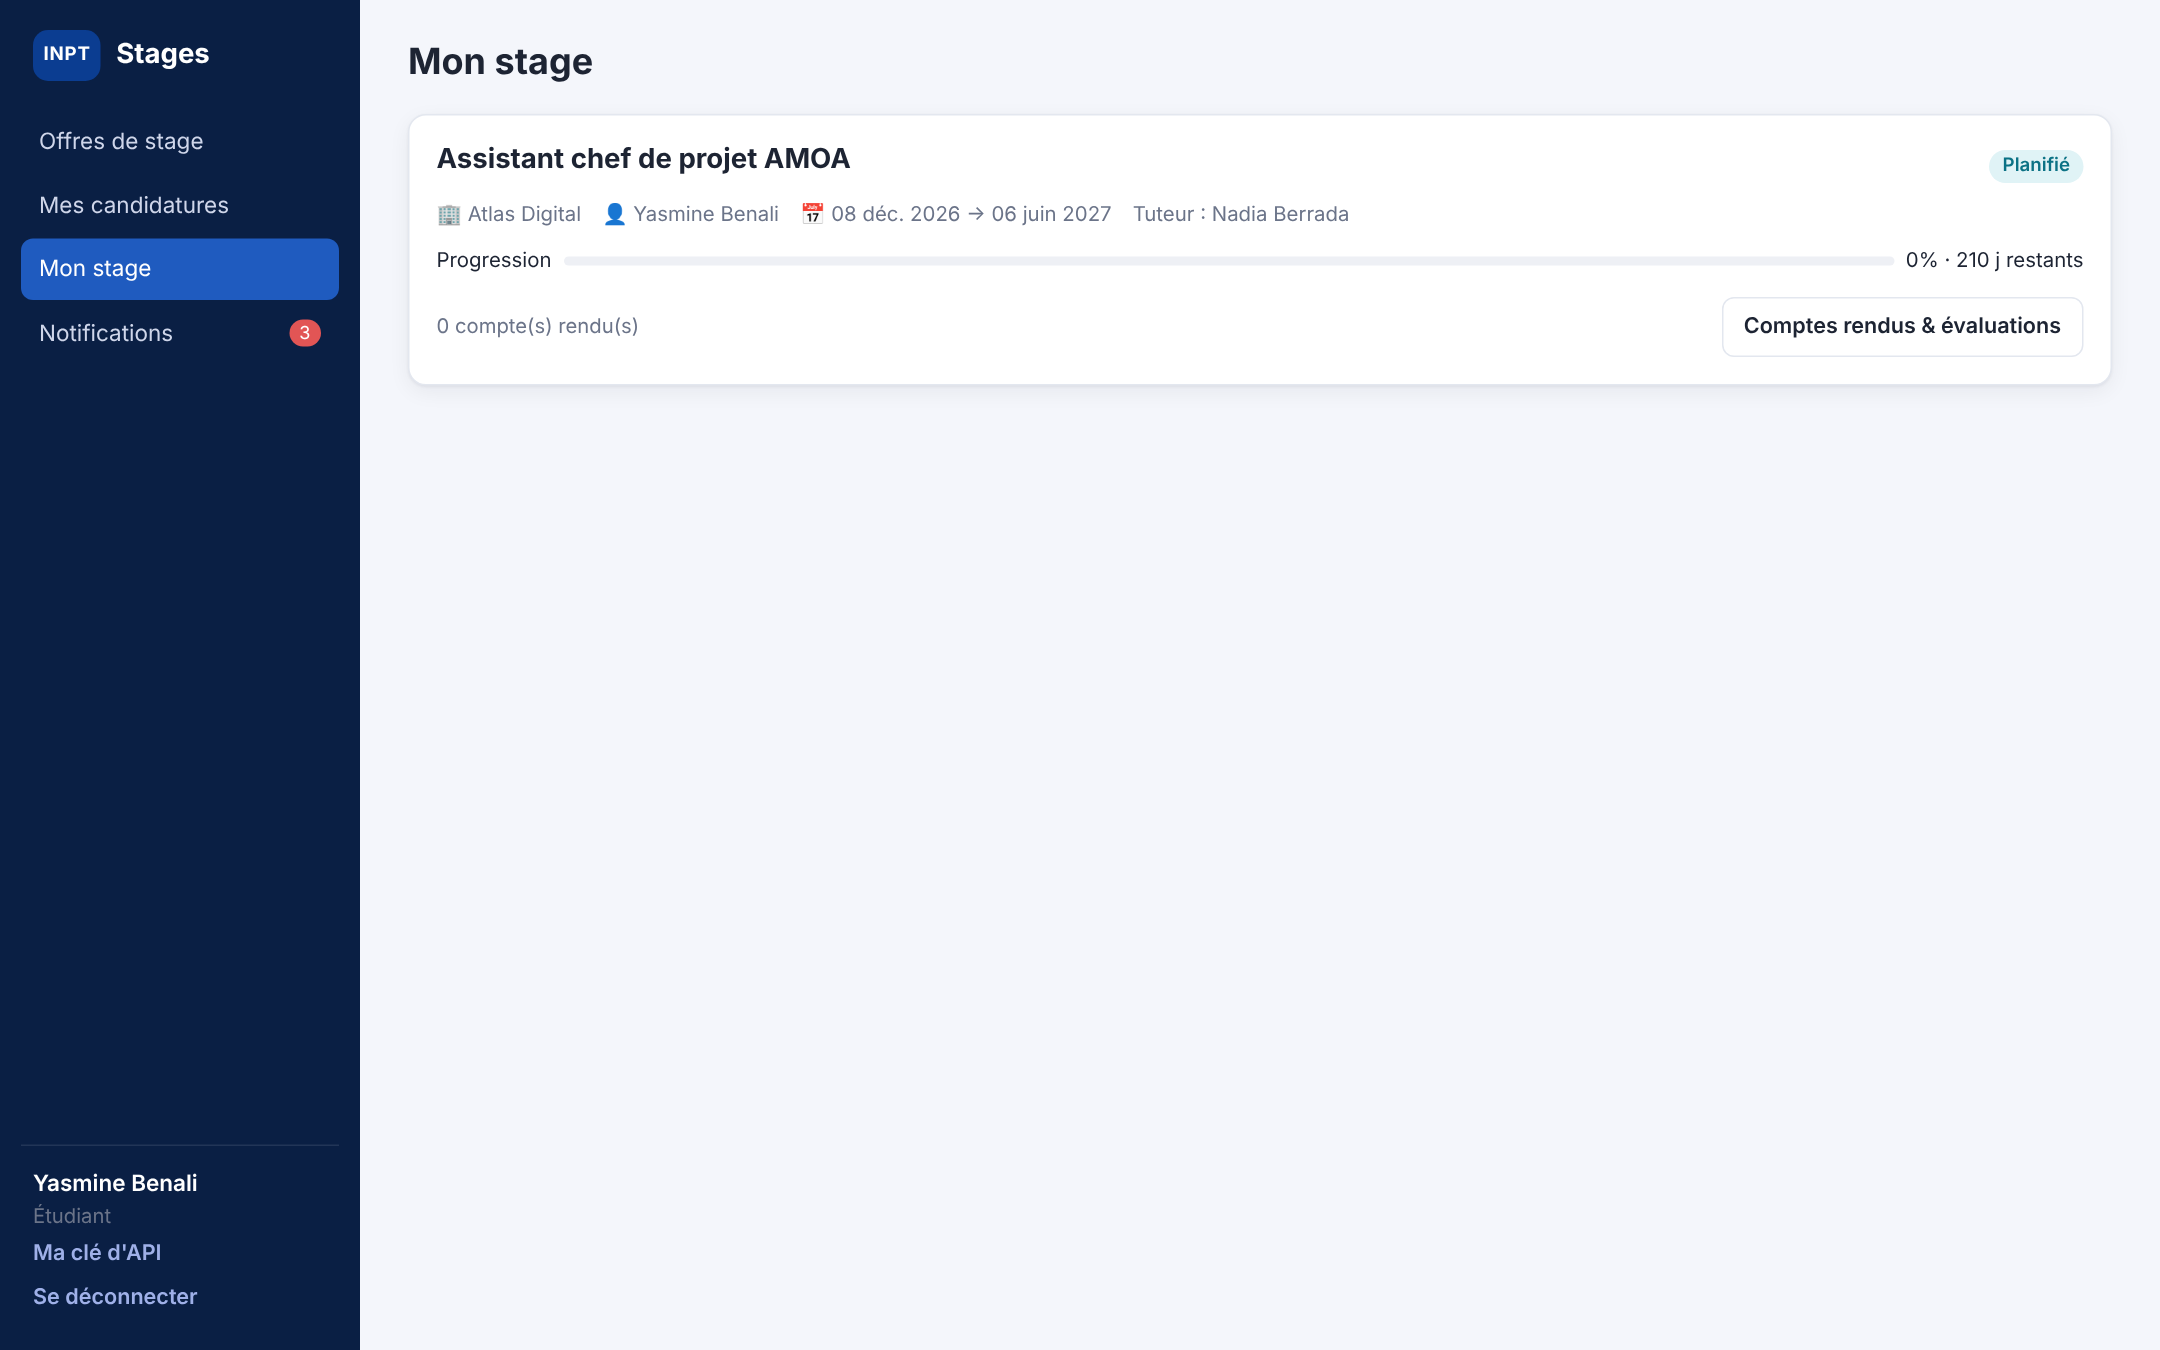
\includegraphics[width=\linewidth]{figures/ui-etudiant-stage.png}\\[-2pt]{\small (b) suivi du stage}
\end{minipage}
\caption{Notifications et suivi du stage}
\end{figure}

\section{E-mails reçus}
\begin{figure}[H]
\centering
\begin{minipage}{0.49\textwidth}\centering
  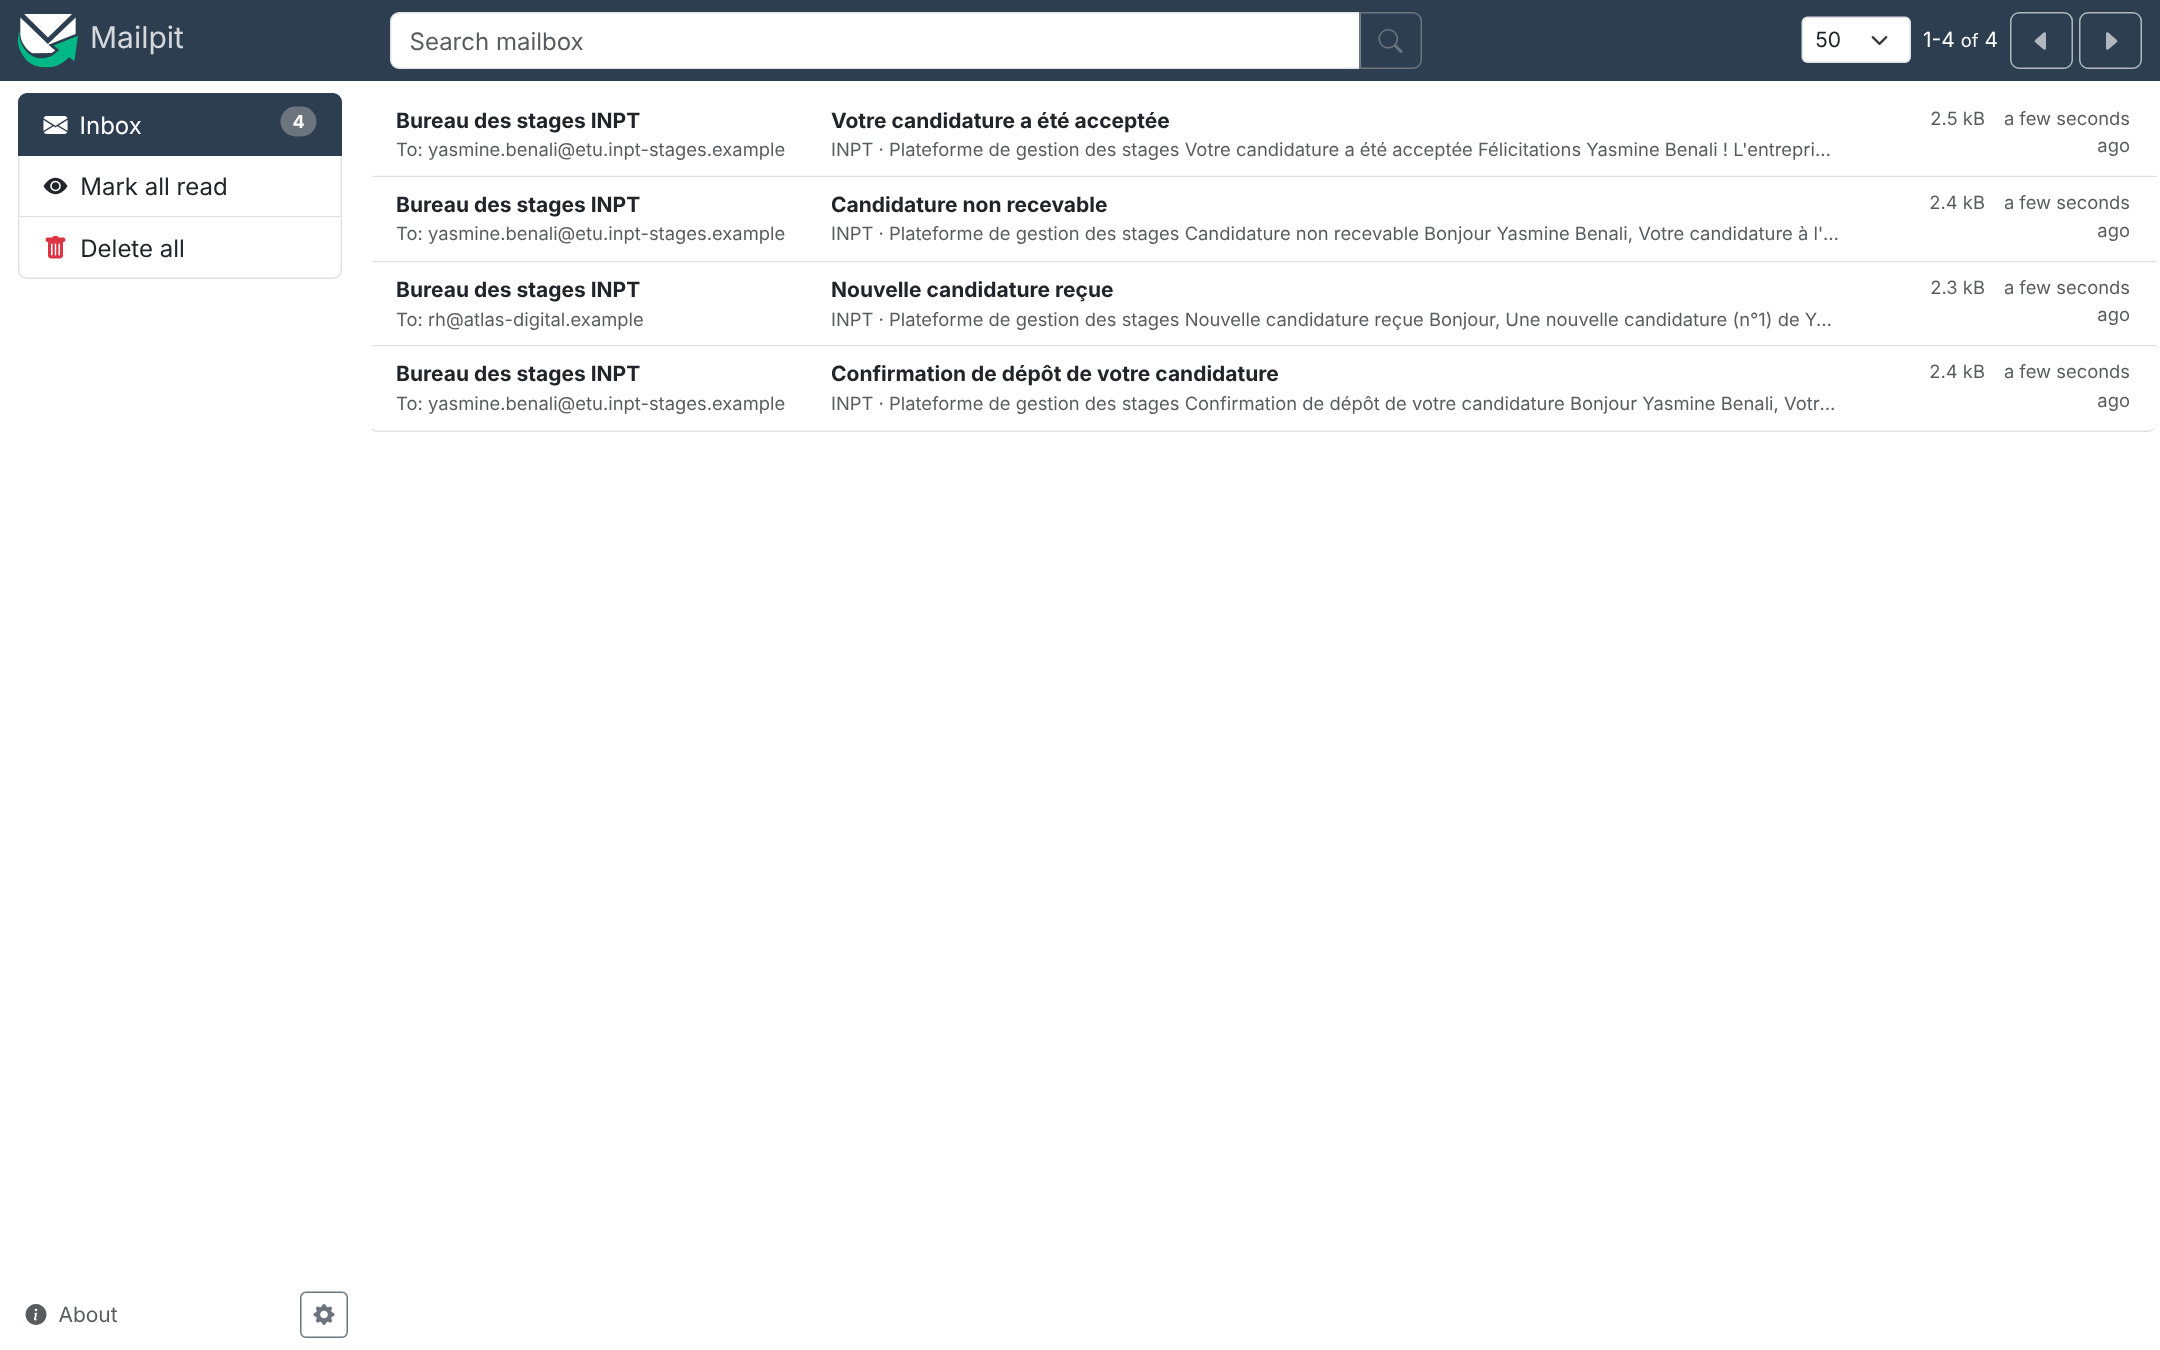
\includegraphics[width=\linewidth]{figures/ui-mailpit-boite.png}\\[-2pt]{\small (a) boîte de réception Mailpit}
\end{minipage}\hfill
\begin{minipage}{0.49\textwidth}\centering
  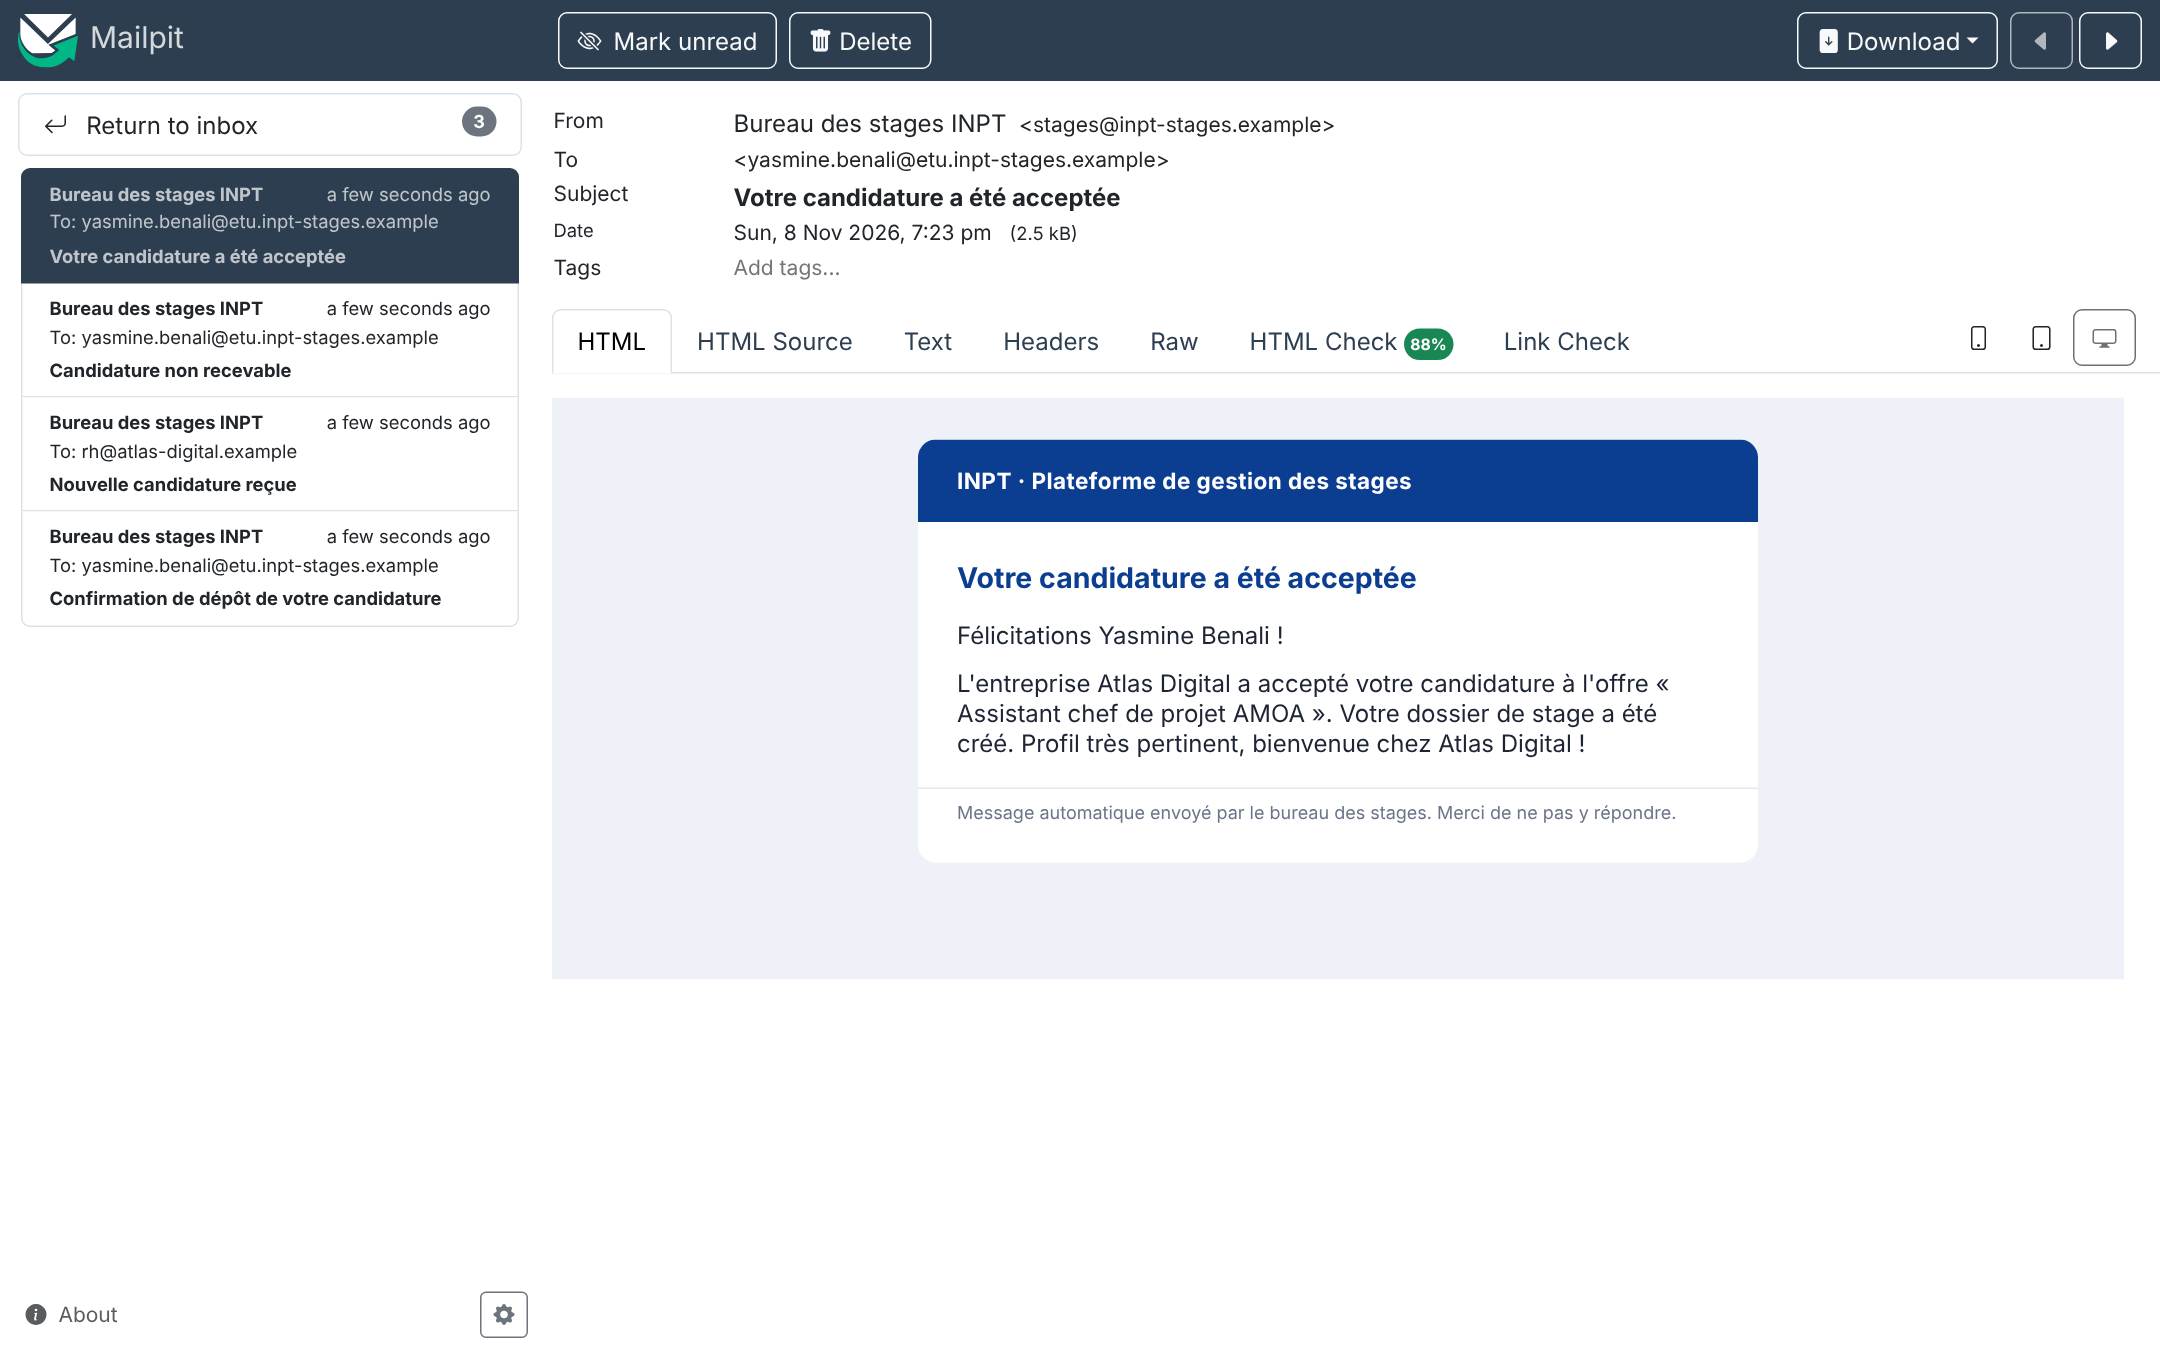
\includegraphics[width=\linewidth]{figures/ui-mailpit-email.png}\\[-2pt]{\small (b) e-mail d'acceptation (HTML)}
\end{minipage}
\caption{Vrais e-mails envoyés en SMTP par le service Notifications et capturés par Mailpit}\label{fig:mailpit}
\end{figure}

\section{Parcours de l'entreprise}
\begin{figure}[H]
\centering
\begin{minipage}{0.49\textwidth}\centering
  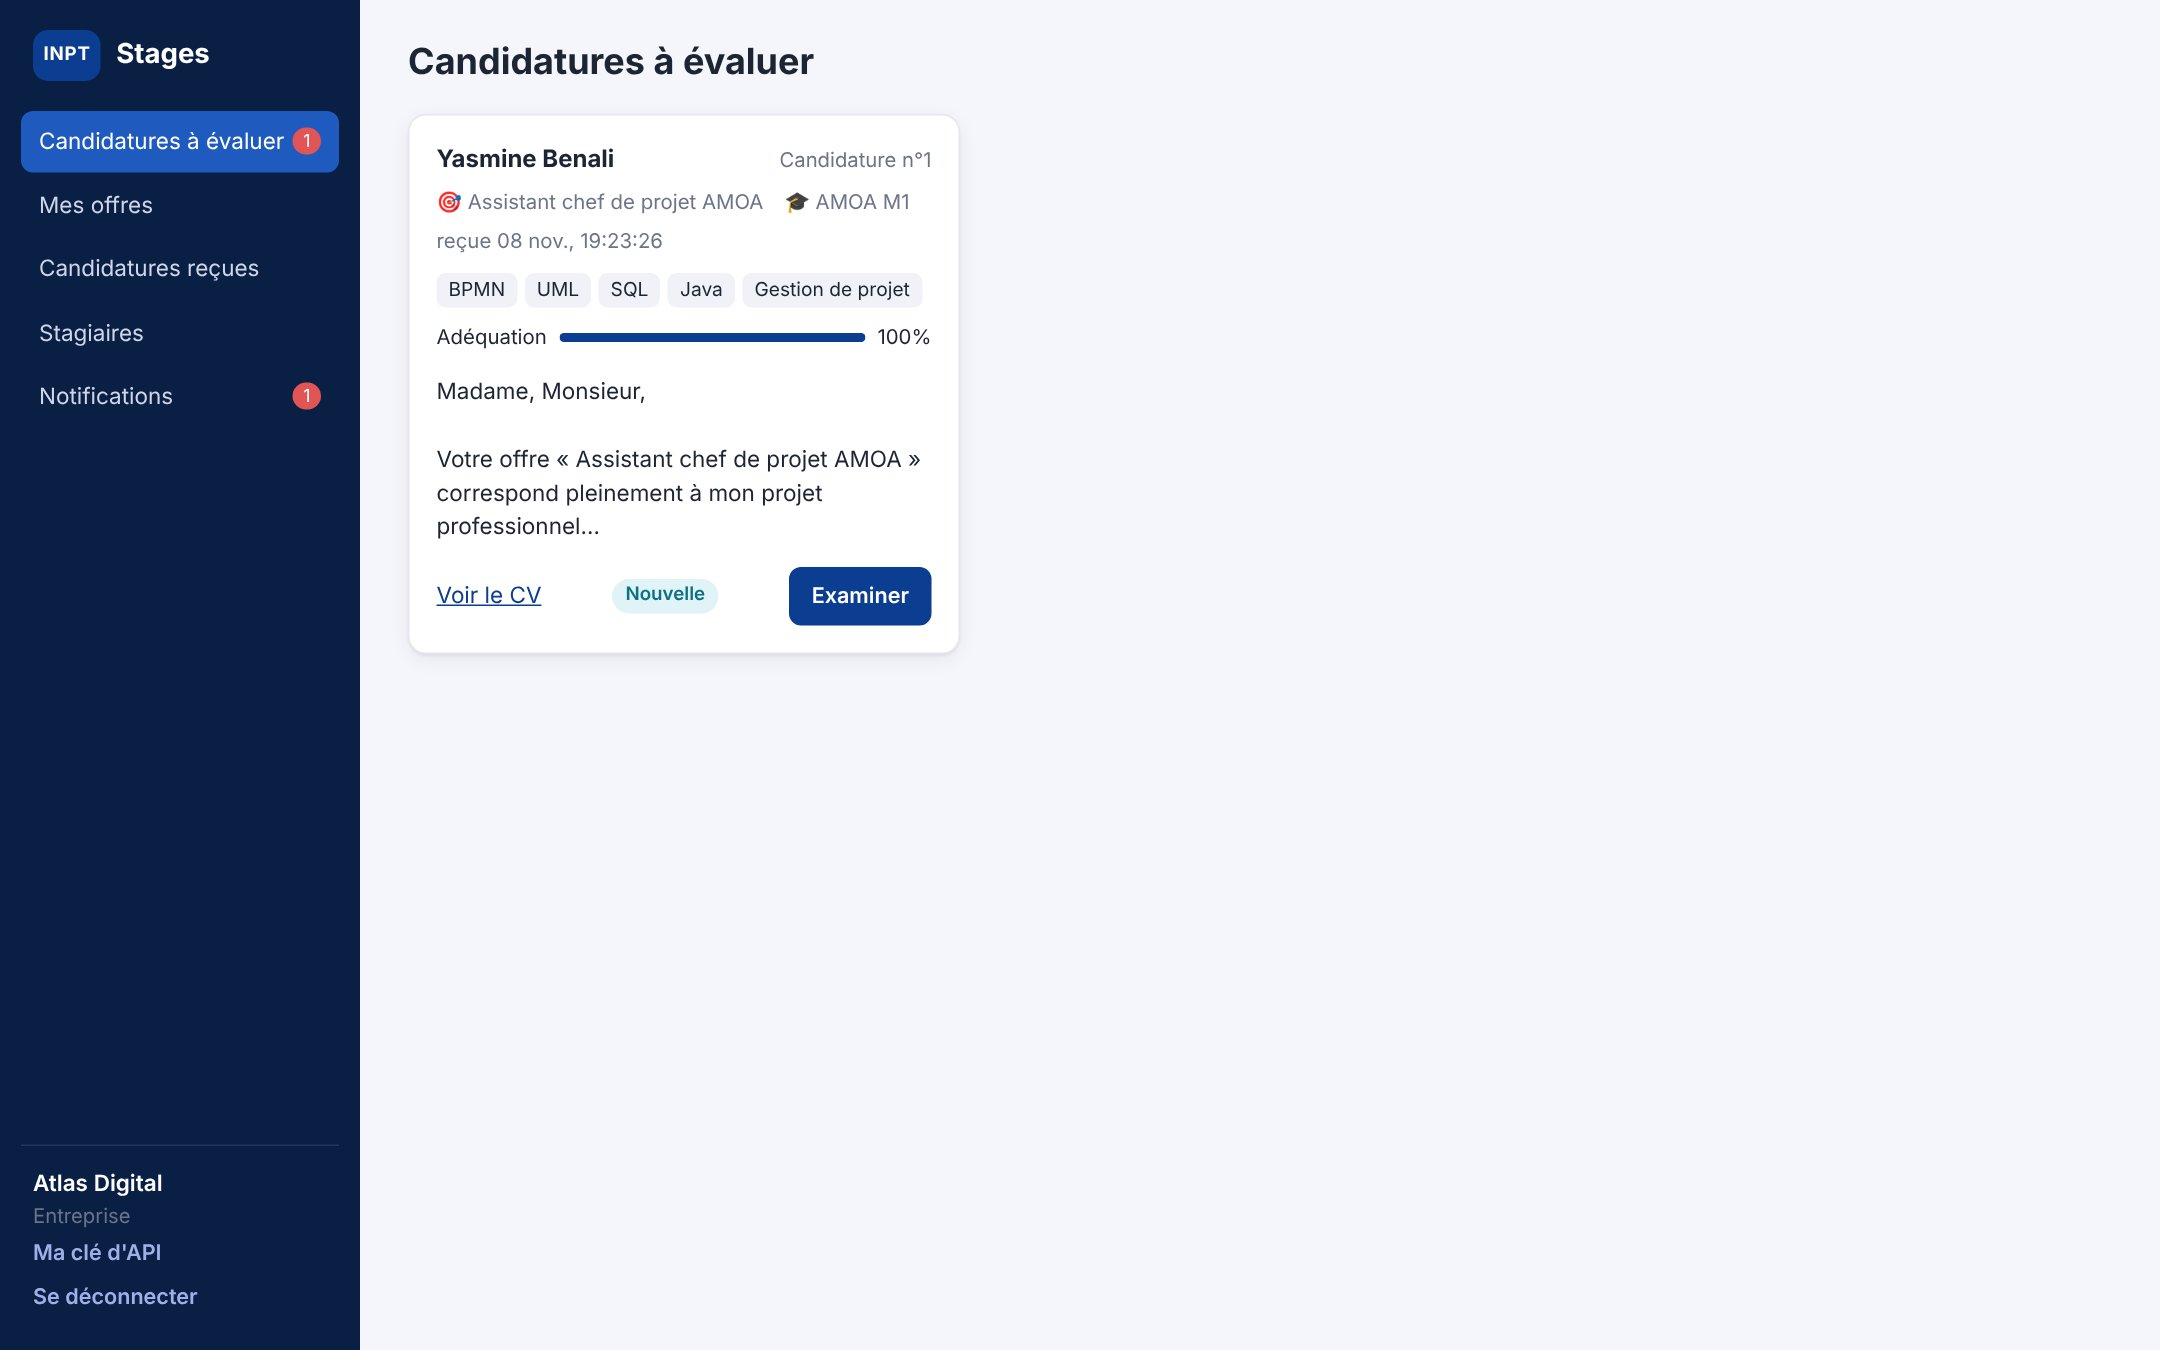
\includegraphics[width=\linewidth]{figures/ui-entreprise-evaluations.png}\\[-2pt]{\small (a) candidatures à évaluer}
\end{minipage}\hfill
\begin{minipage}{0.49\textwidth}\centering
  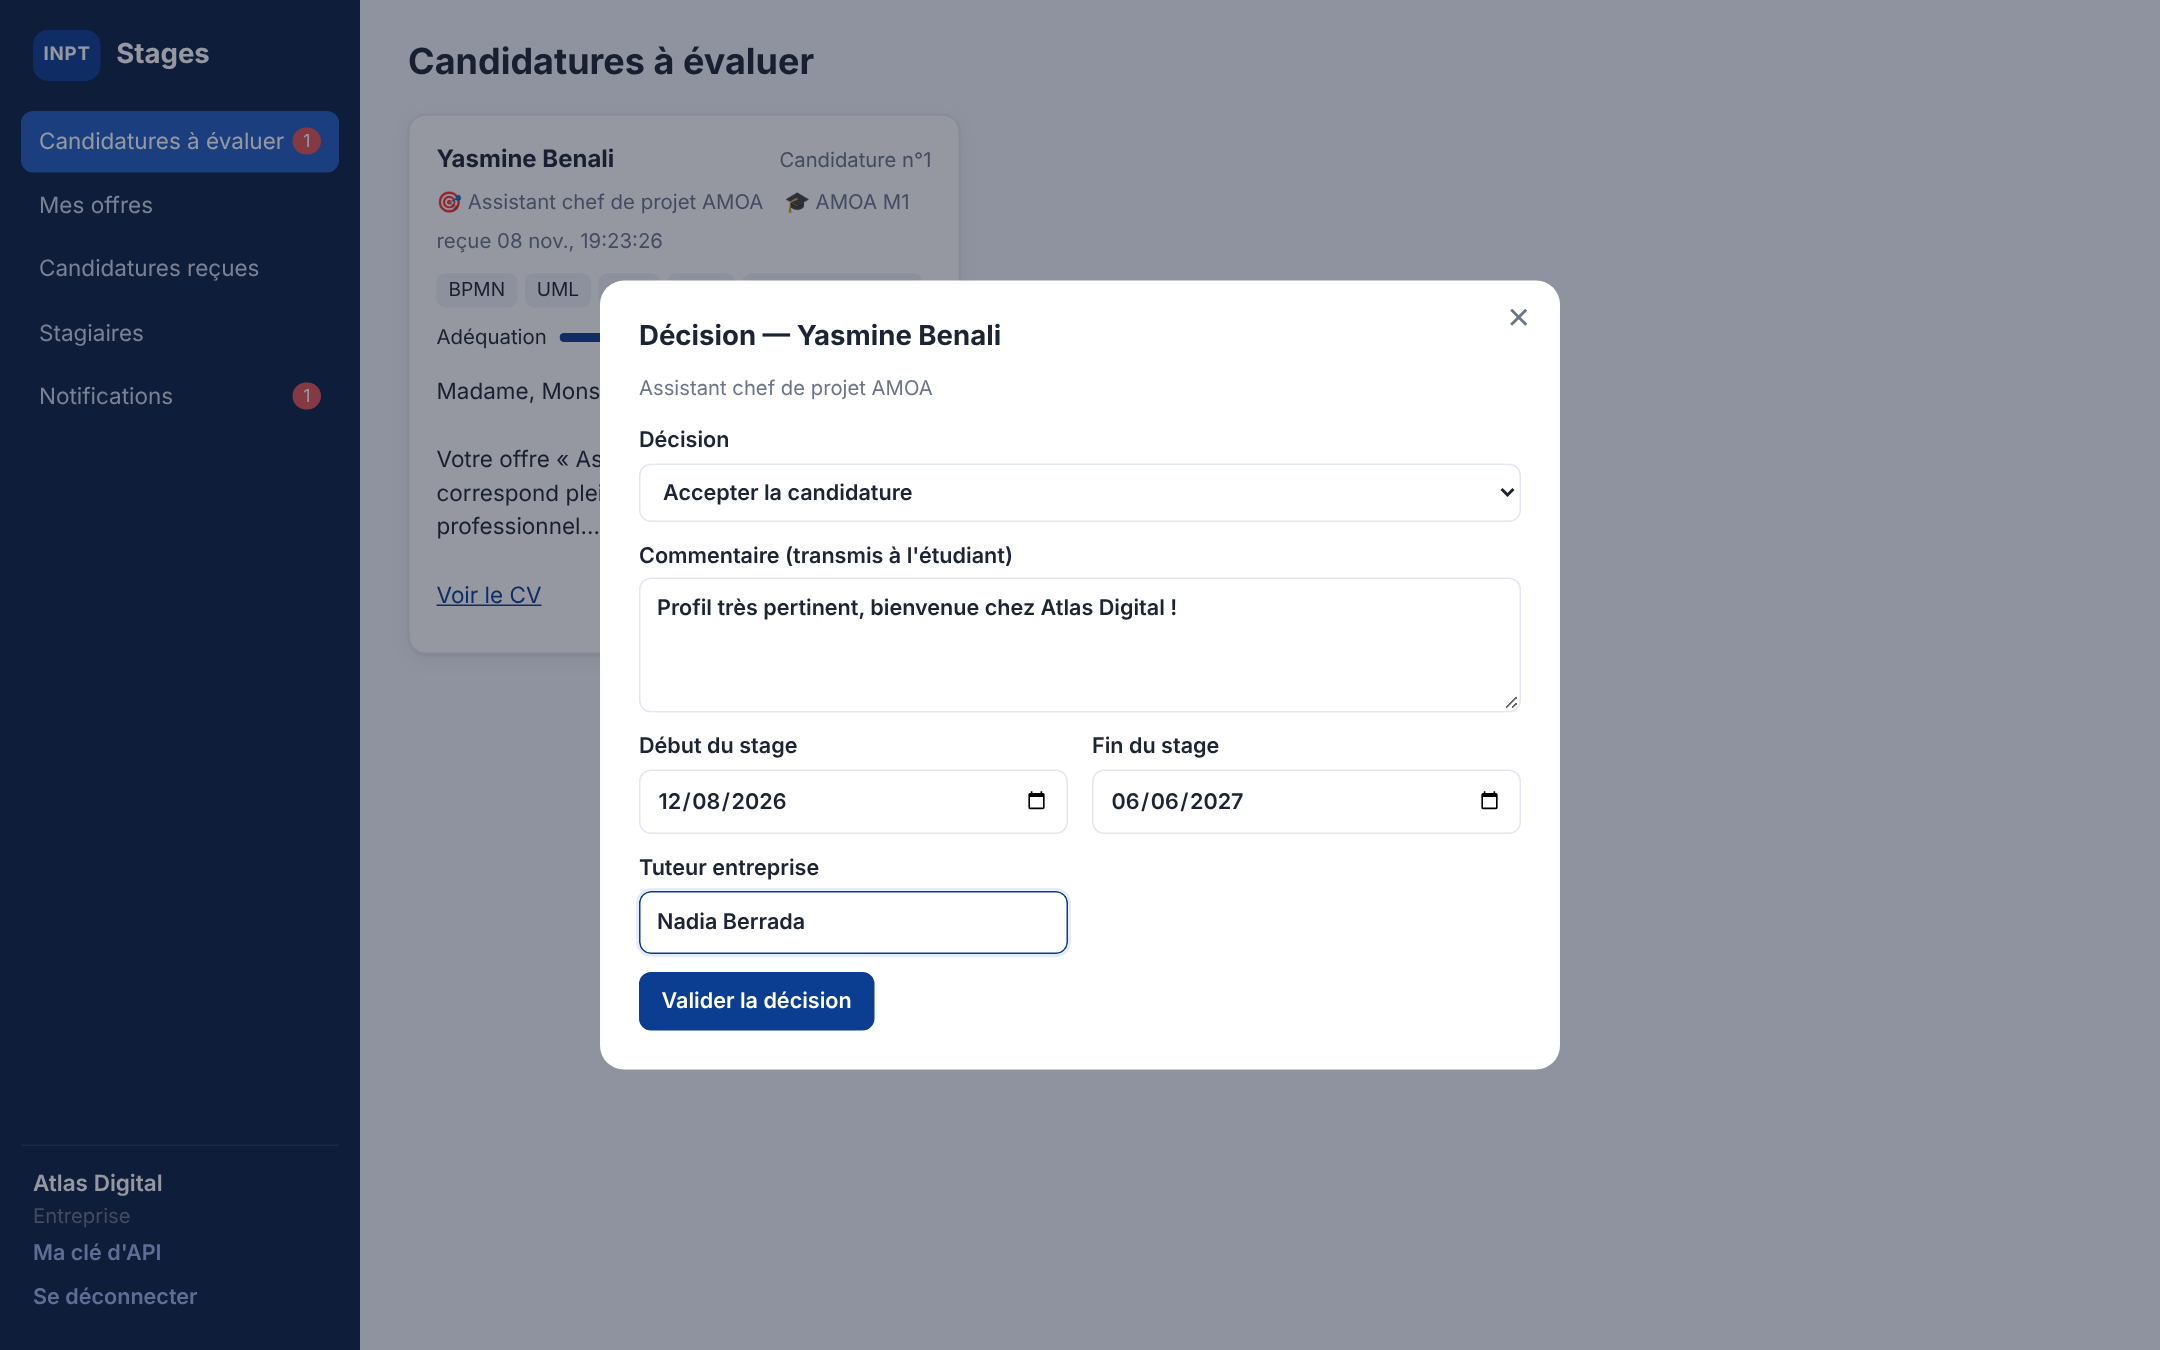
\includegraphics[width=\linewidth]{figures/ui-entreprise-decision.png}\\[-2pt]{\small (b) décision (tâche humaine BPMN)}
\end{minipage}
\caption{Évaluation d'une candidature par l'entreprise : « Examiner » prend la candidature en charge, puis la décision est rendue}
\end{figure}

\section{Parcours du responsable}
\begin{figure}[H]
\centering
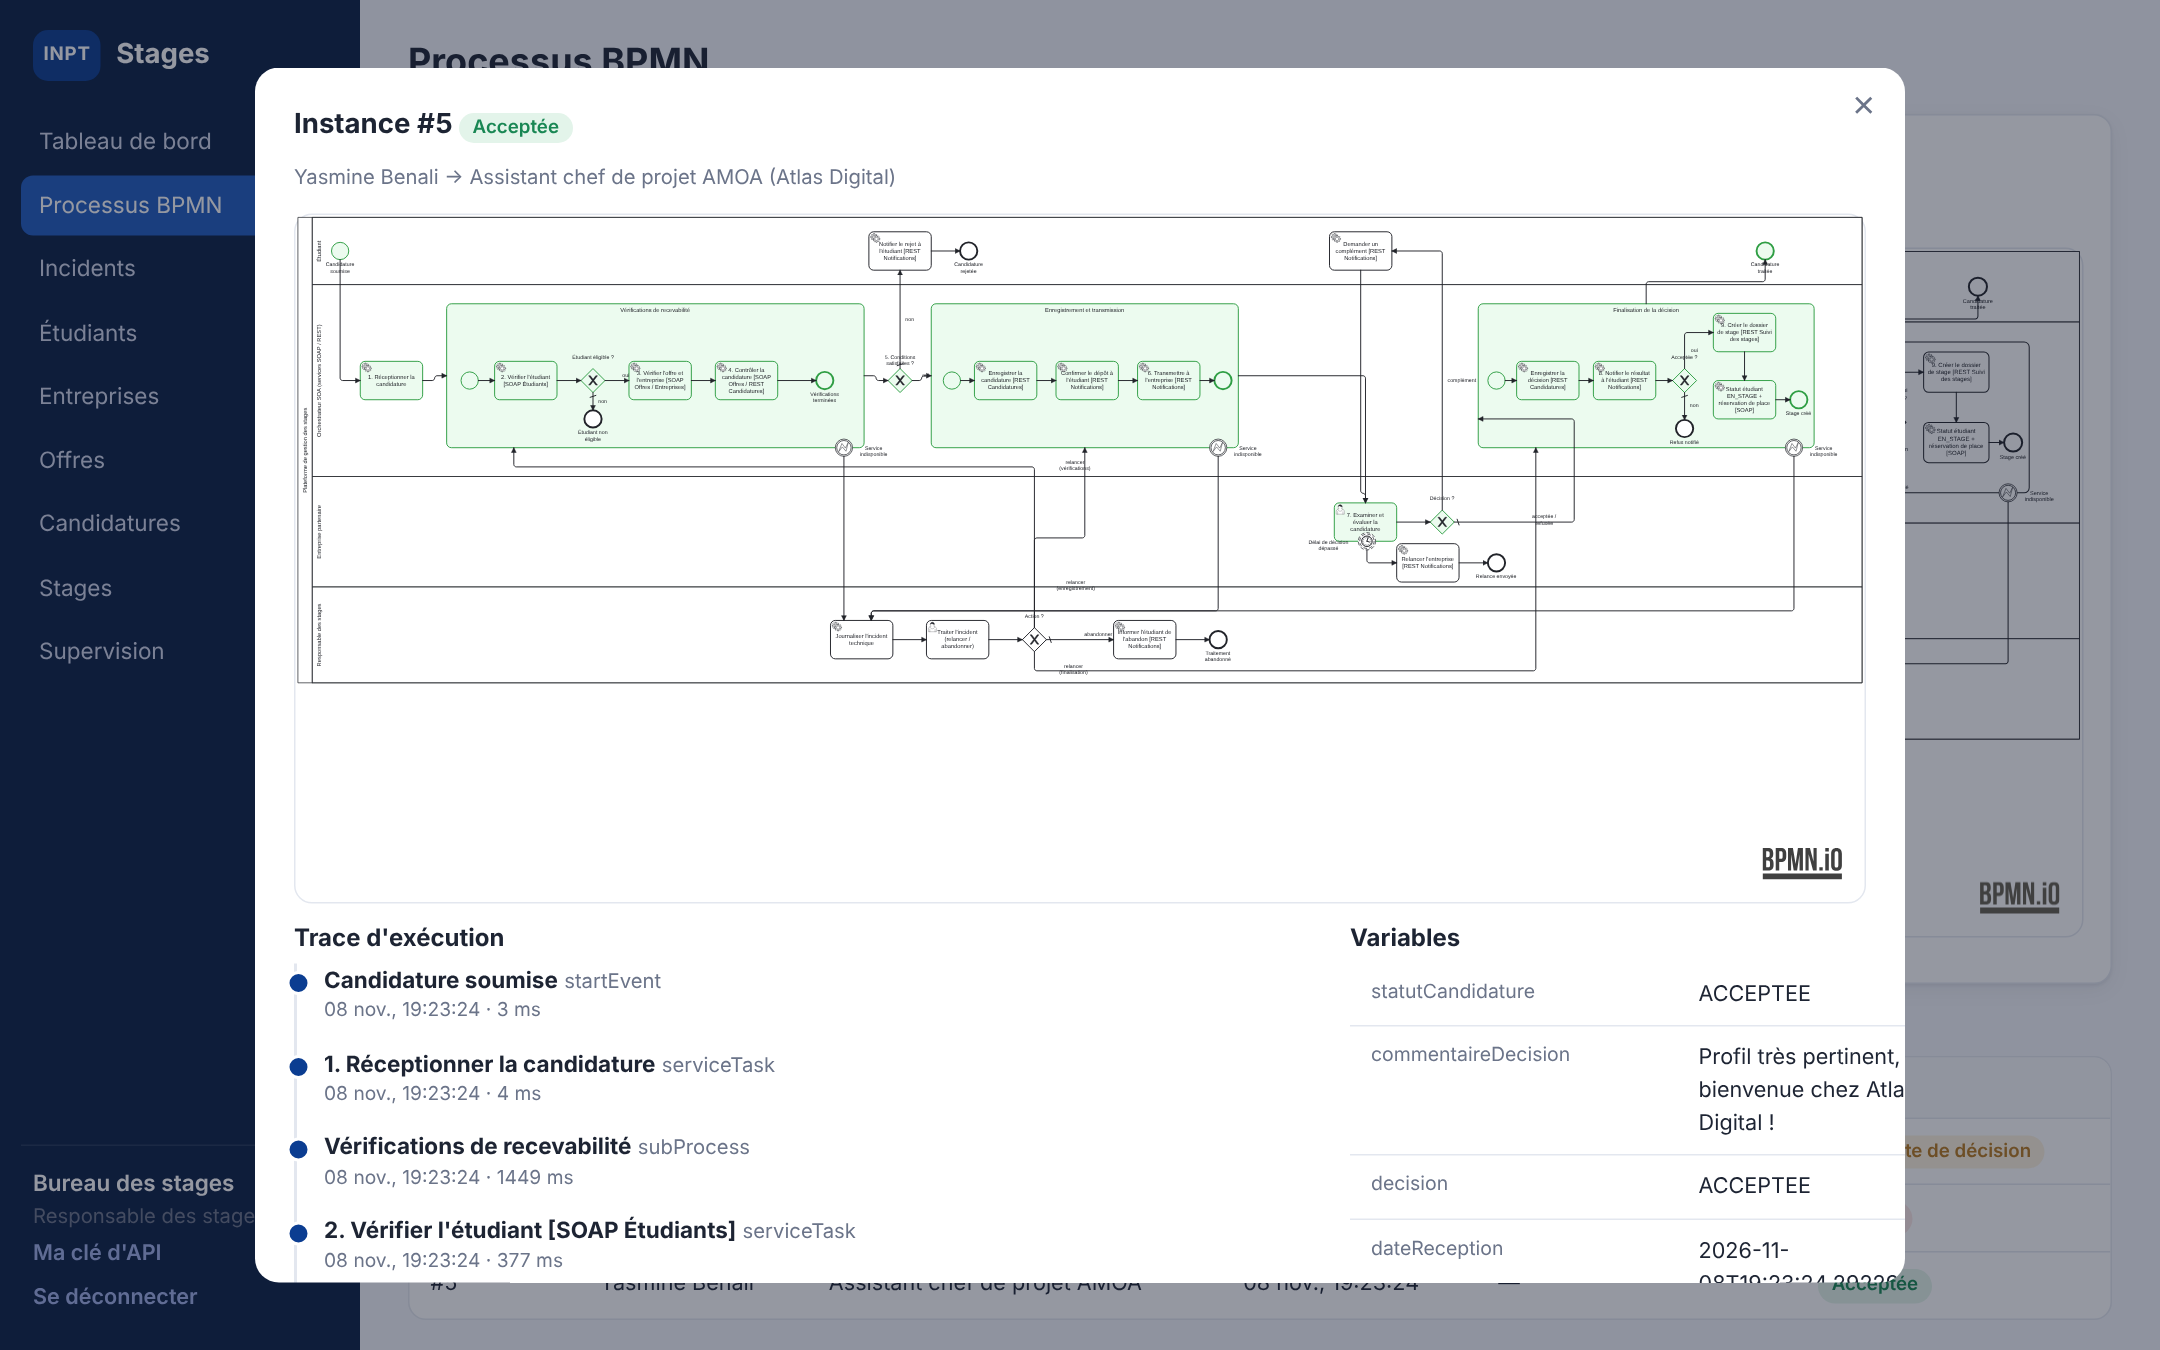
\includegraphics[width=0.92\textwidth]{figures/ui-admin-instance.png}
\caption{Suivi d'une instance : activités traversées en vert sur le diagramme, trace d'exécution et variables}\label{fig:ui-instance}
\end{figure}

\begin{figure}[H]
\centering
\begin{minipage}{0.49\textwidth}\centering
  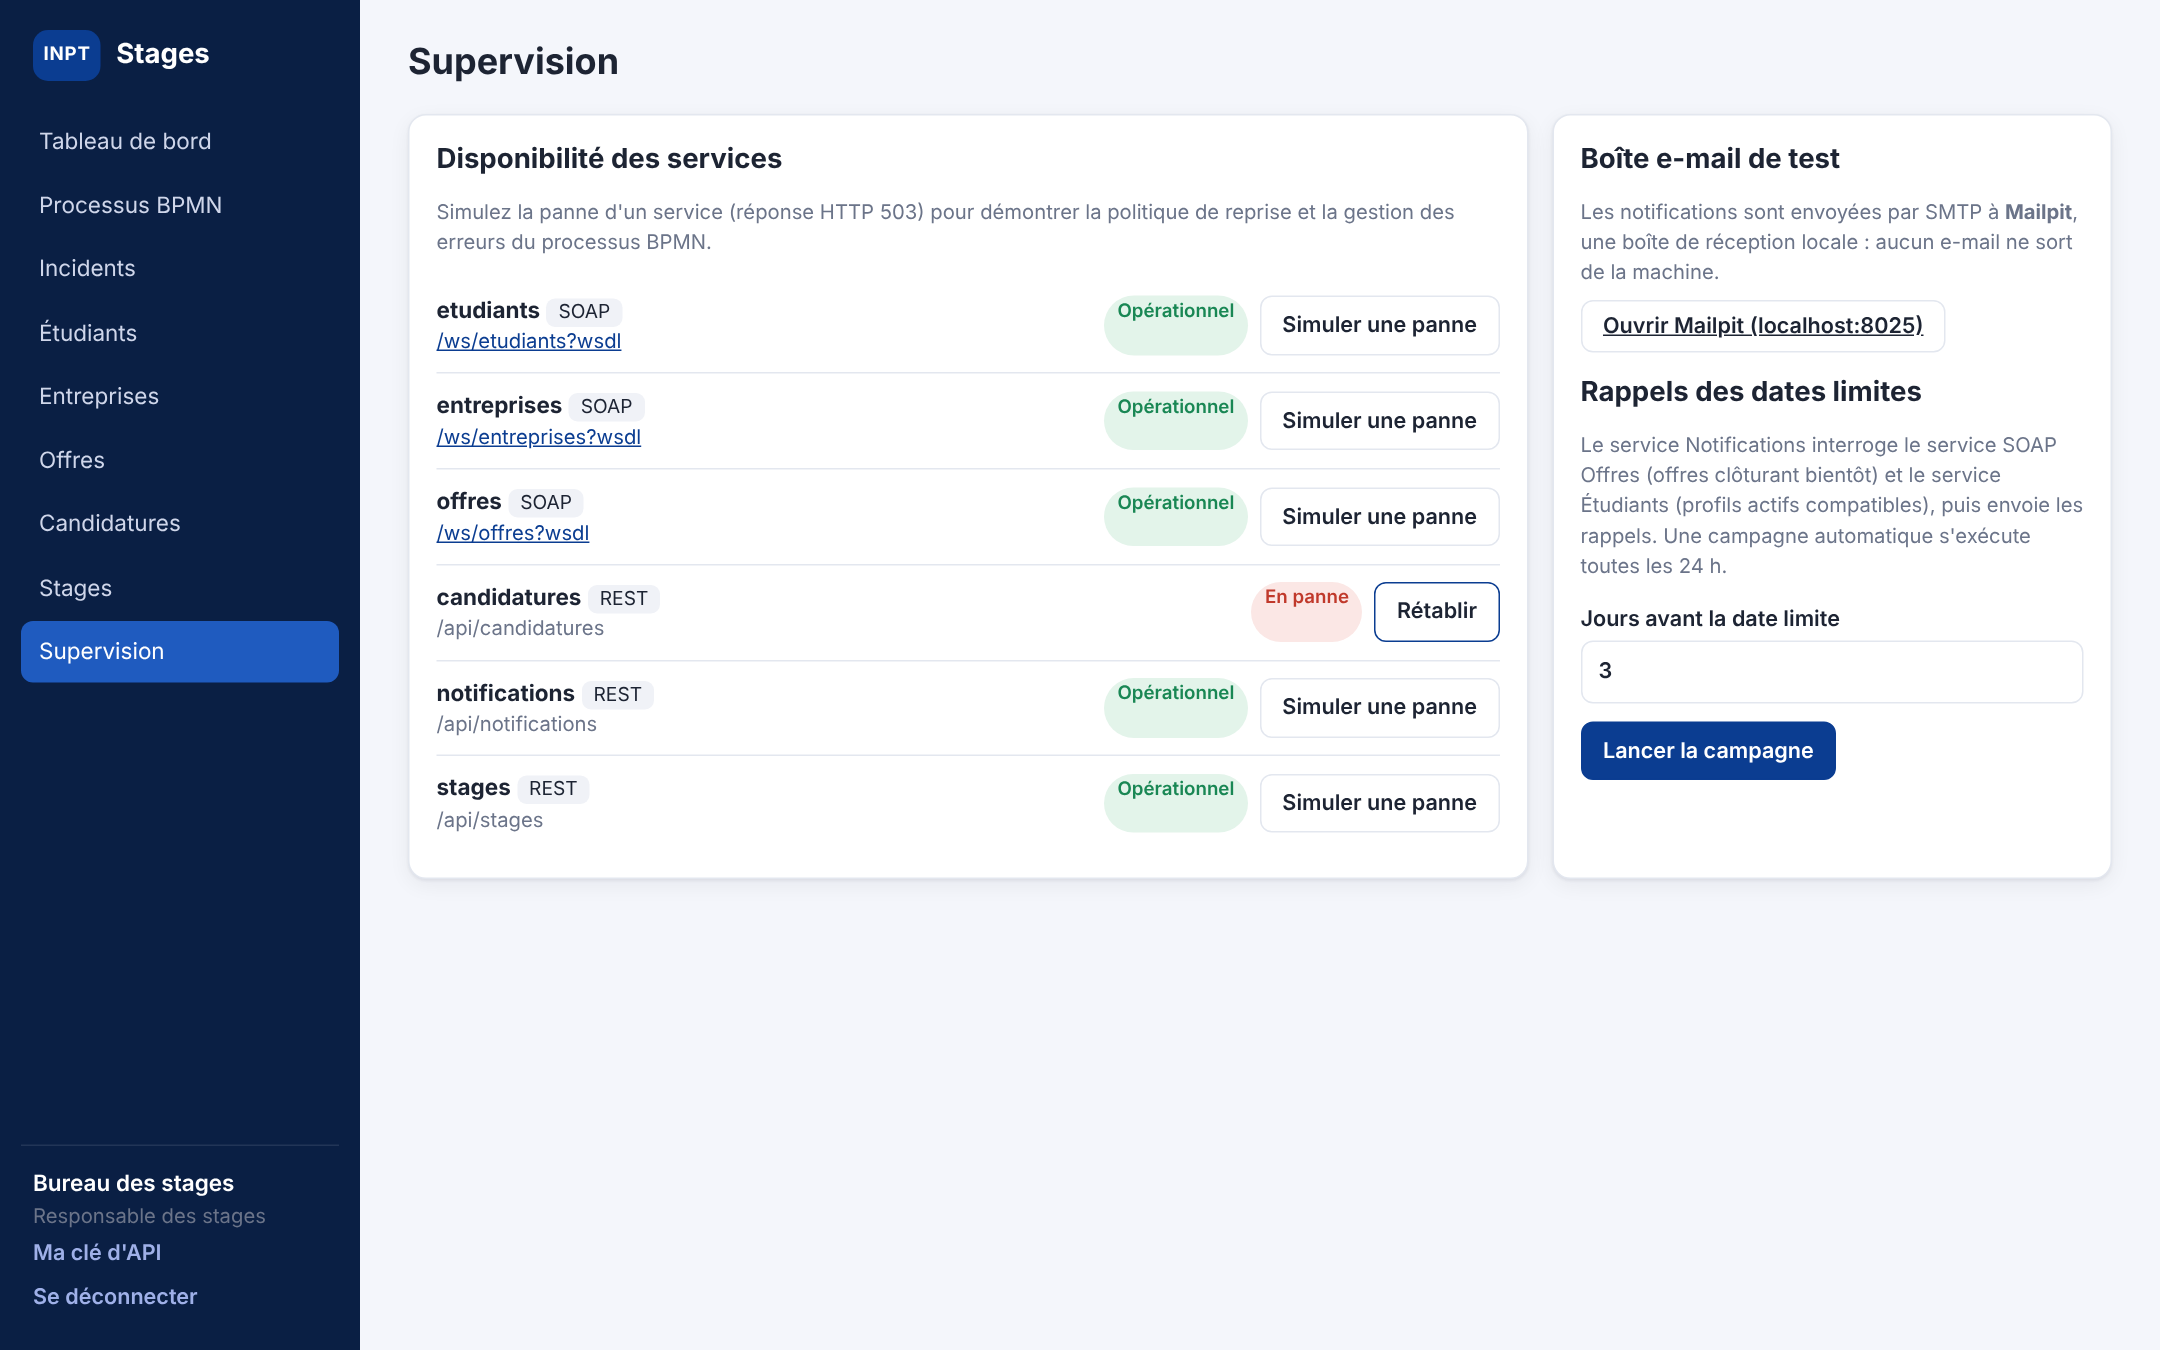
\includegraphics[width=\linewidth]{figures/ui-admin-supervision.png}\\[-2pt]{\small (a) simulation d'une panne}
\end{minipage}\hfill
\begin{minipage}{0.49\textwidth}\centering
  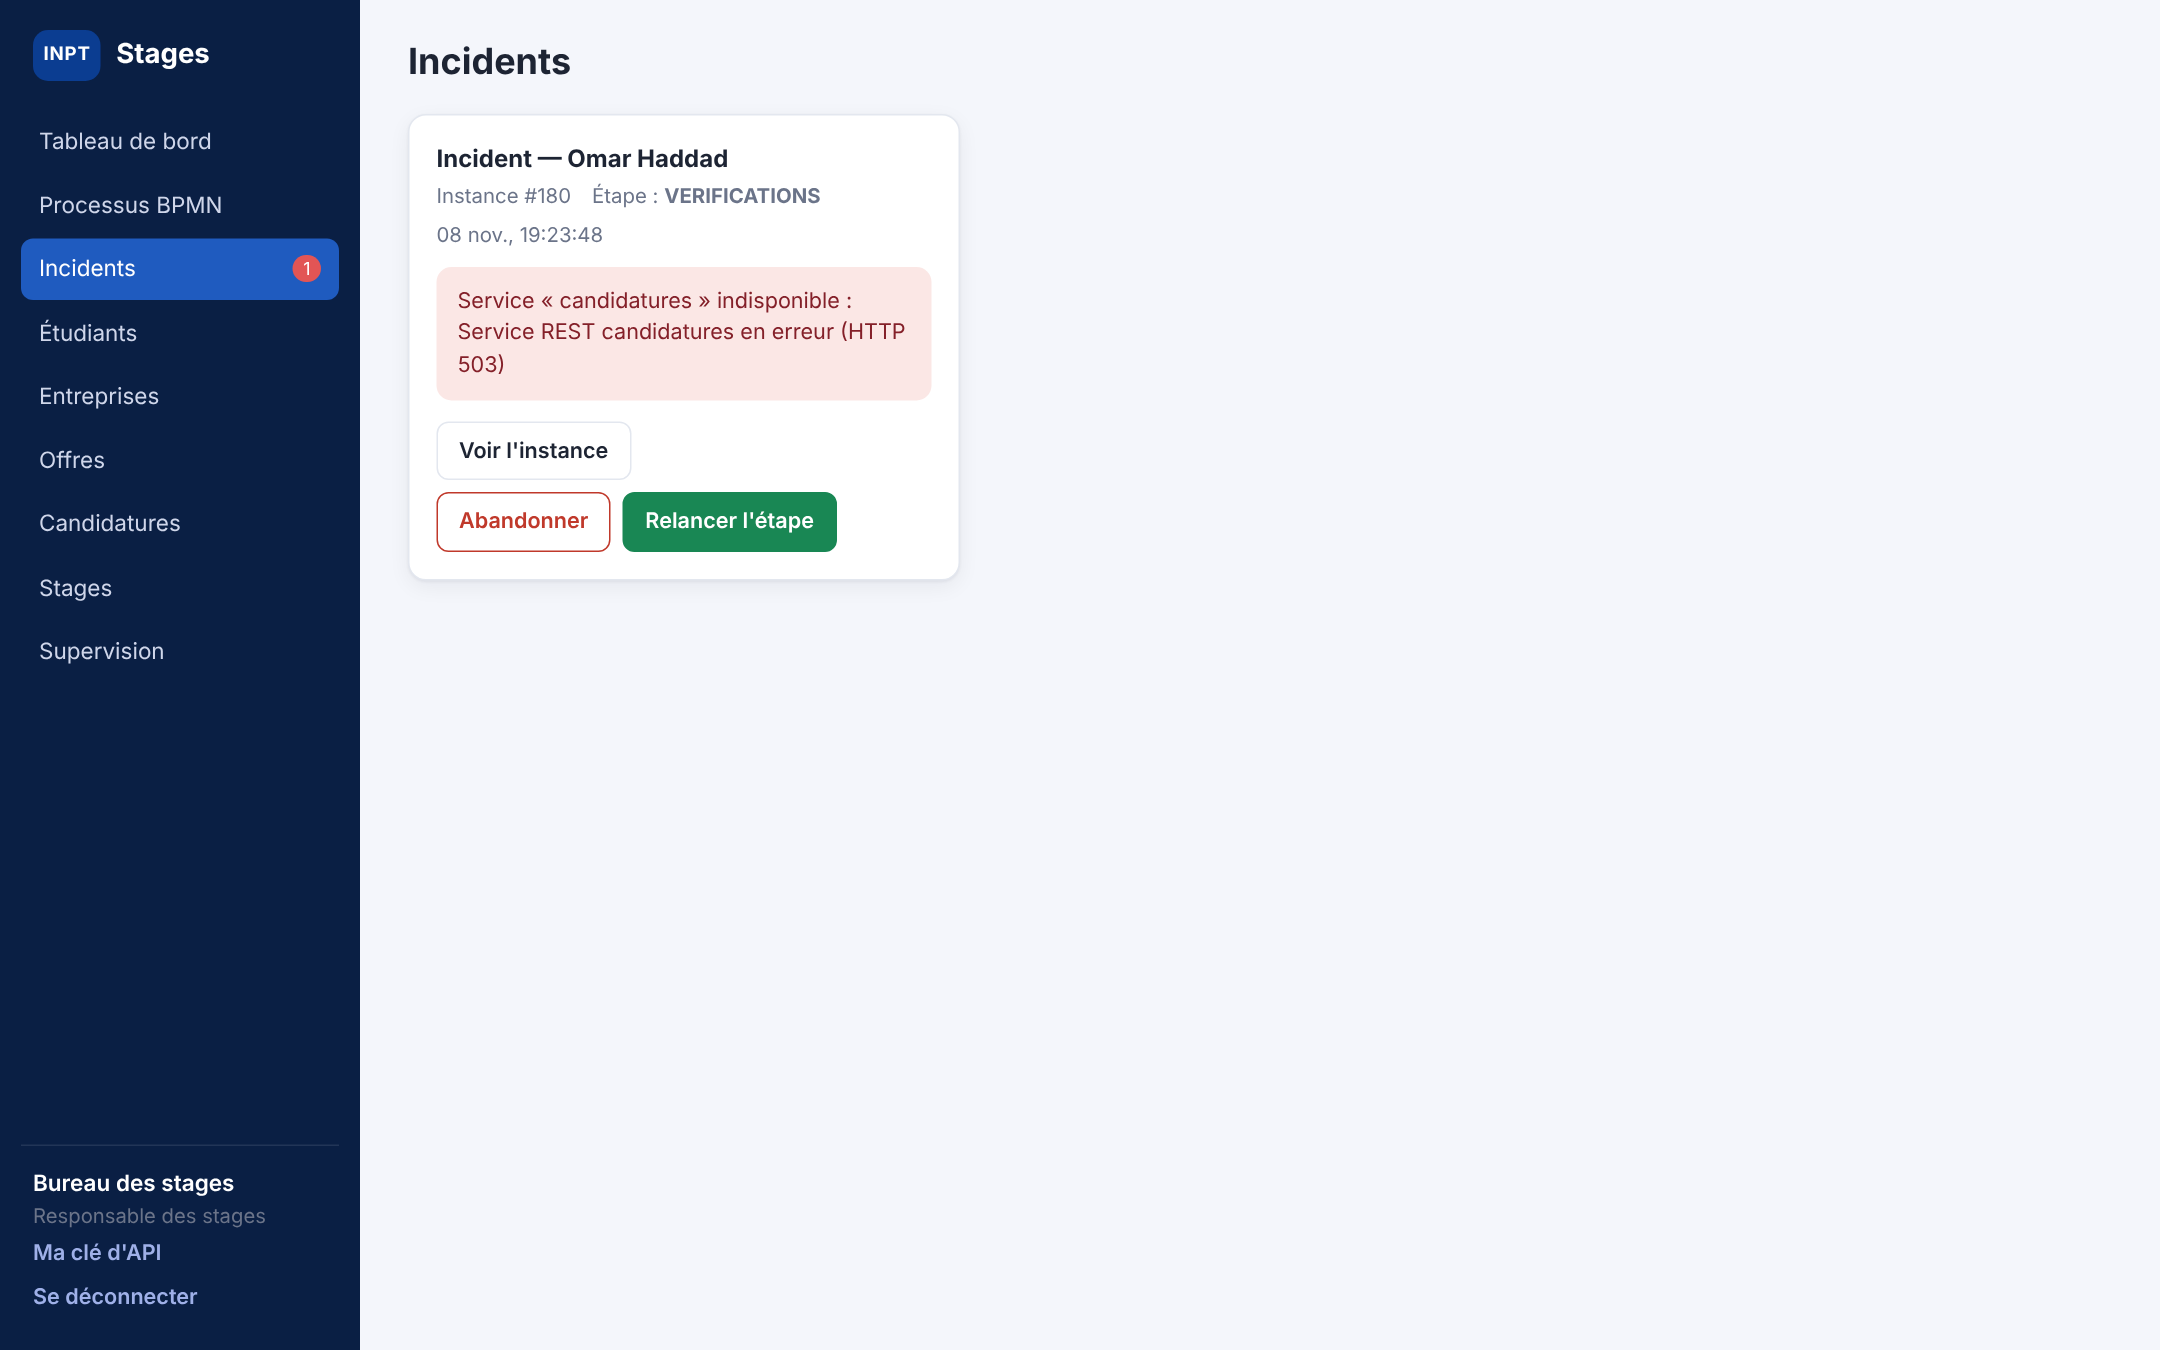
\includegraphics[width=\linewidth]{figures/ui-admin-incidents.png}\\[-2pt]{\small (b) incident à traiter}
\end{minipage}
\caption{Gestion d'une indisponibilité de service depuis l'interface}
\end{figure}

\begin{figure}[H]
\centering
\begin{minipage}{0.49\textwidth}\centering
  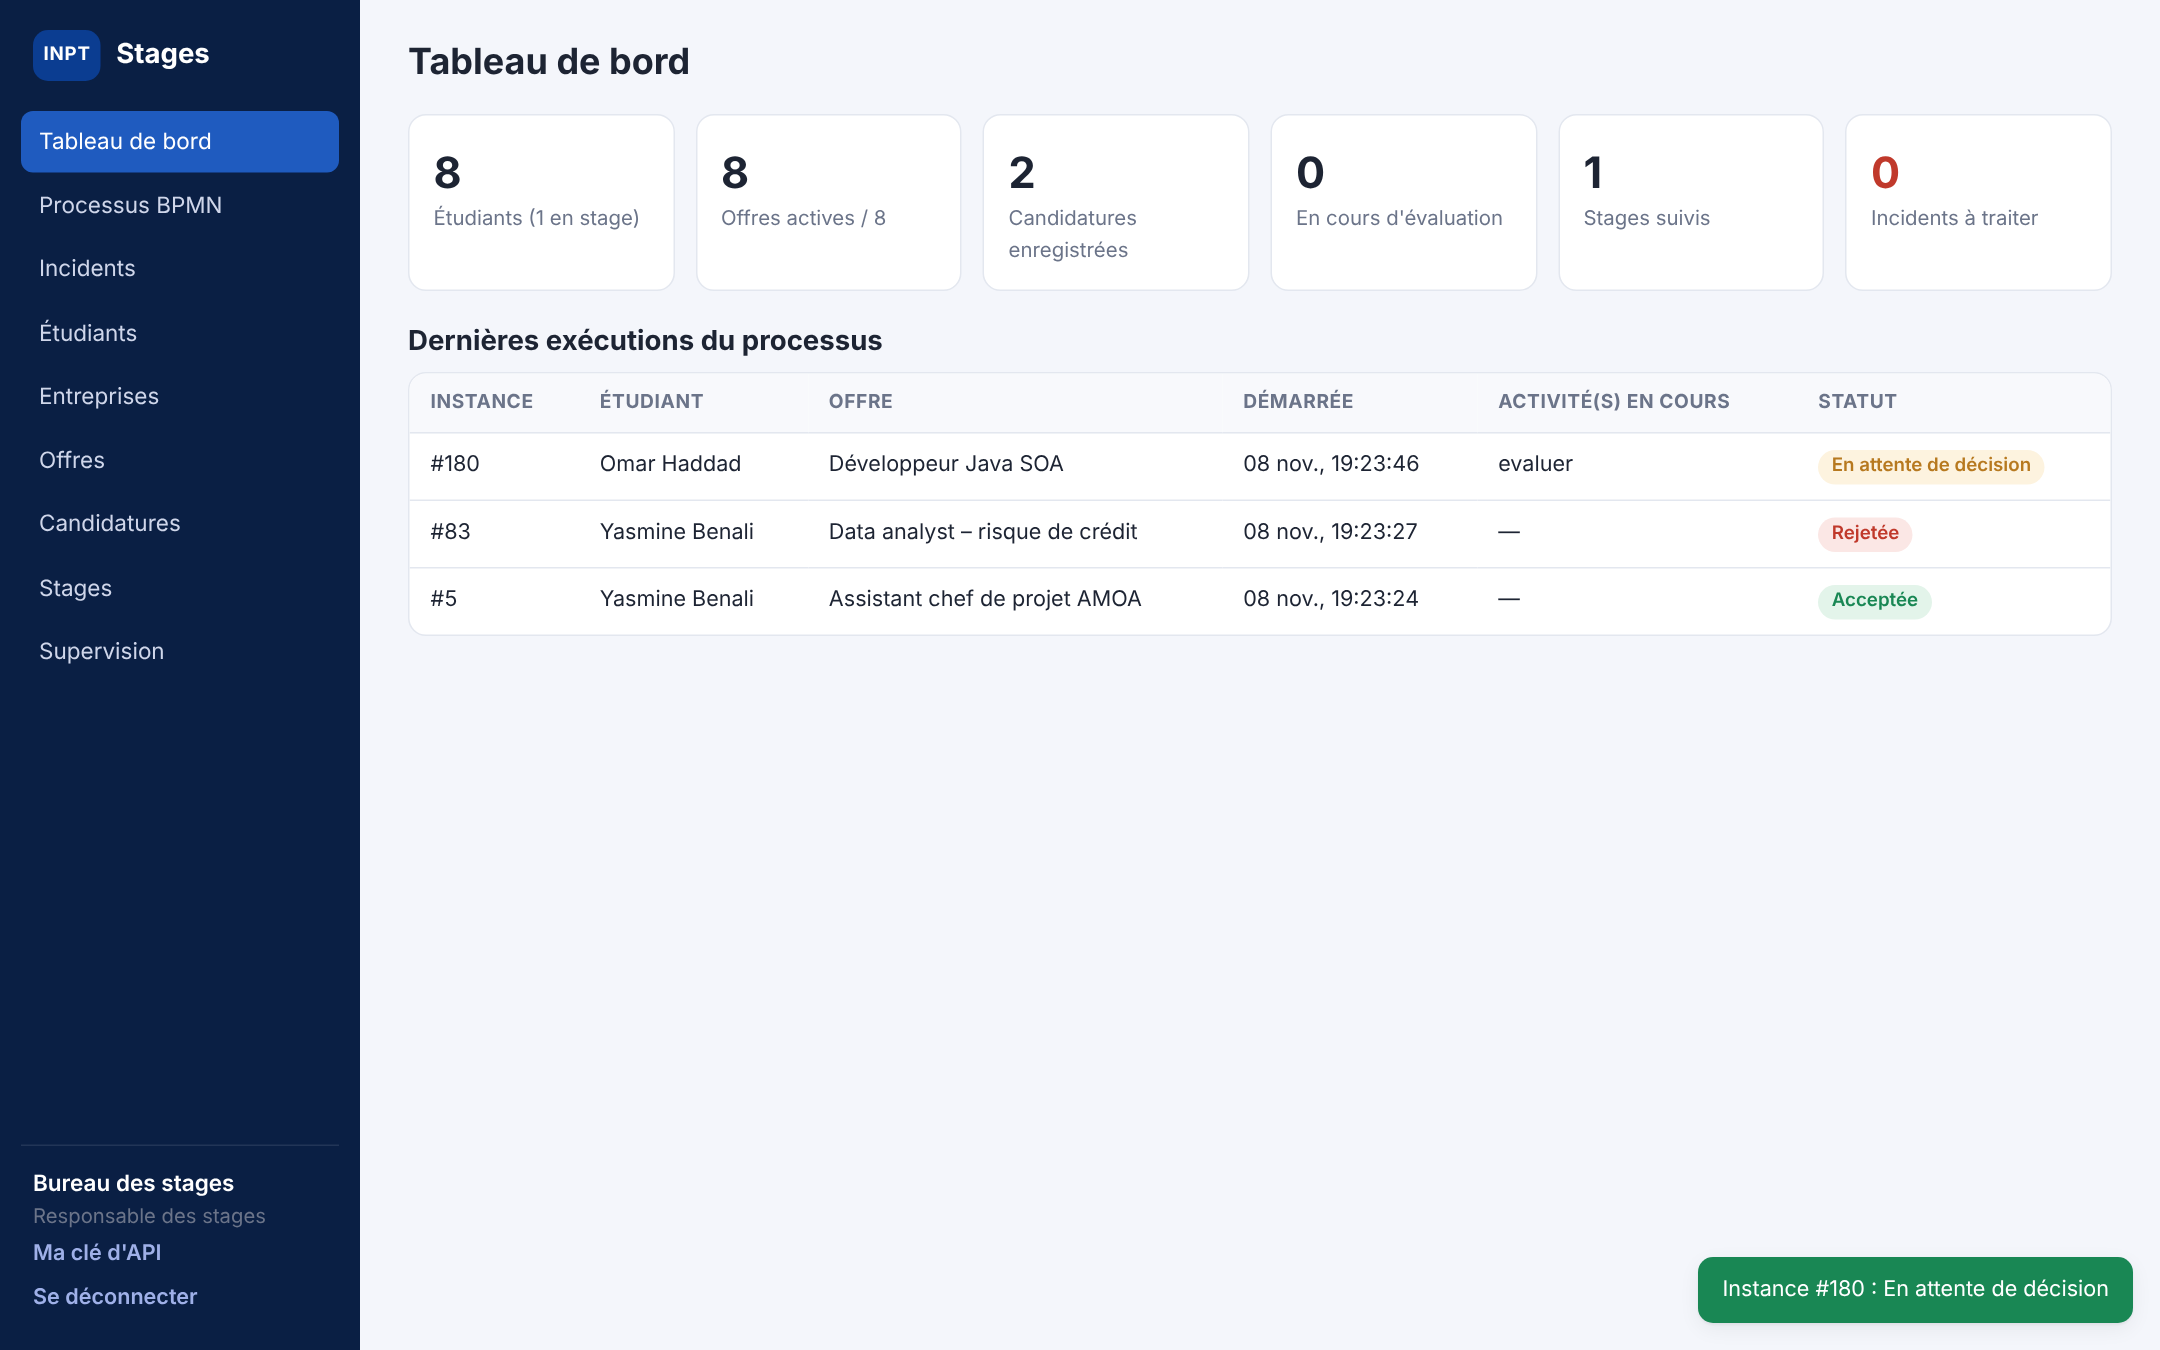
\includegraphics[width=\linewidth]{figures/ui-admin-tableau.png}\\[-2pt]{\small (a) tableau de bord}
\end{minipage}\hfill
\begin{minipage}{0.49\textwidth}\centering
  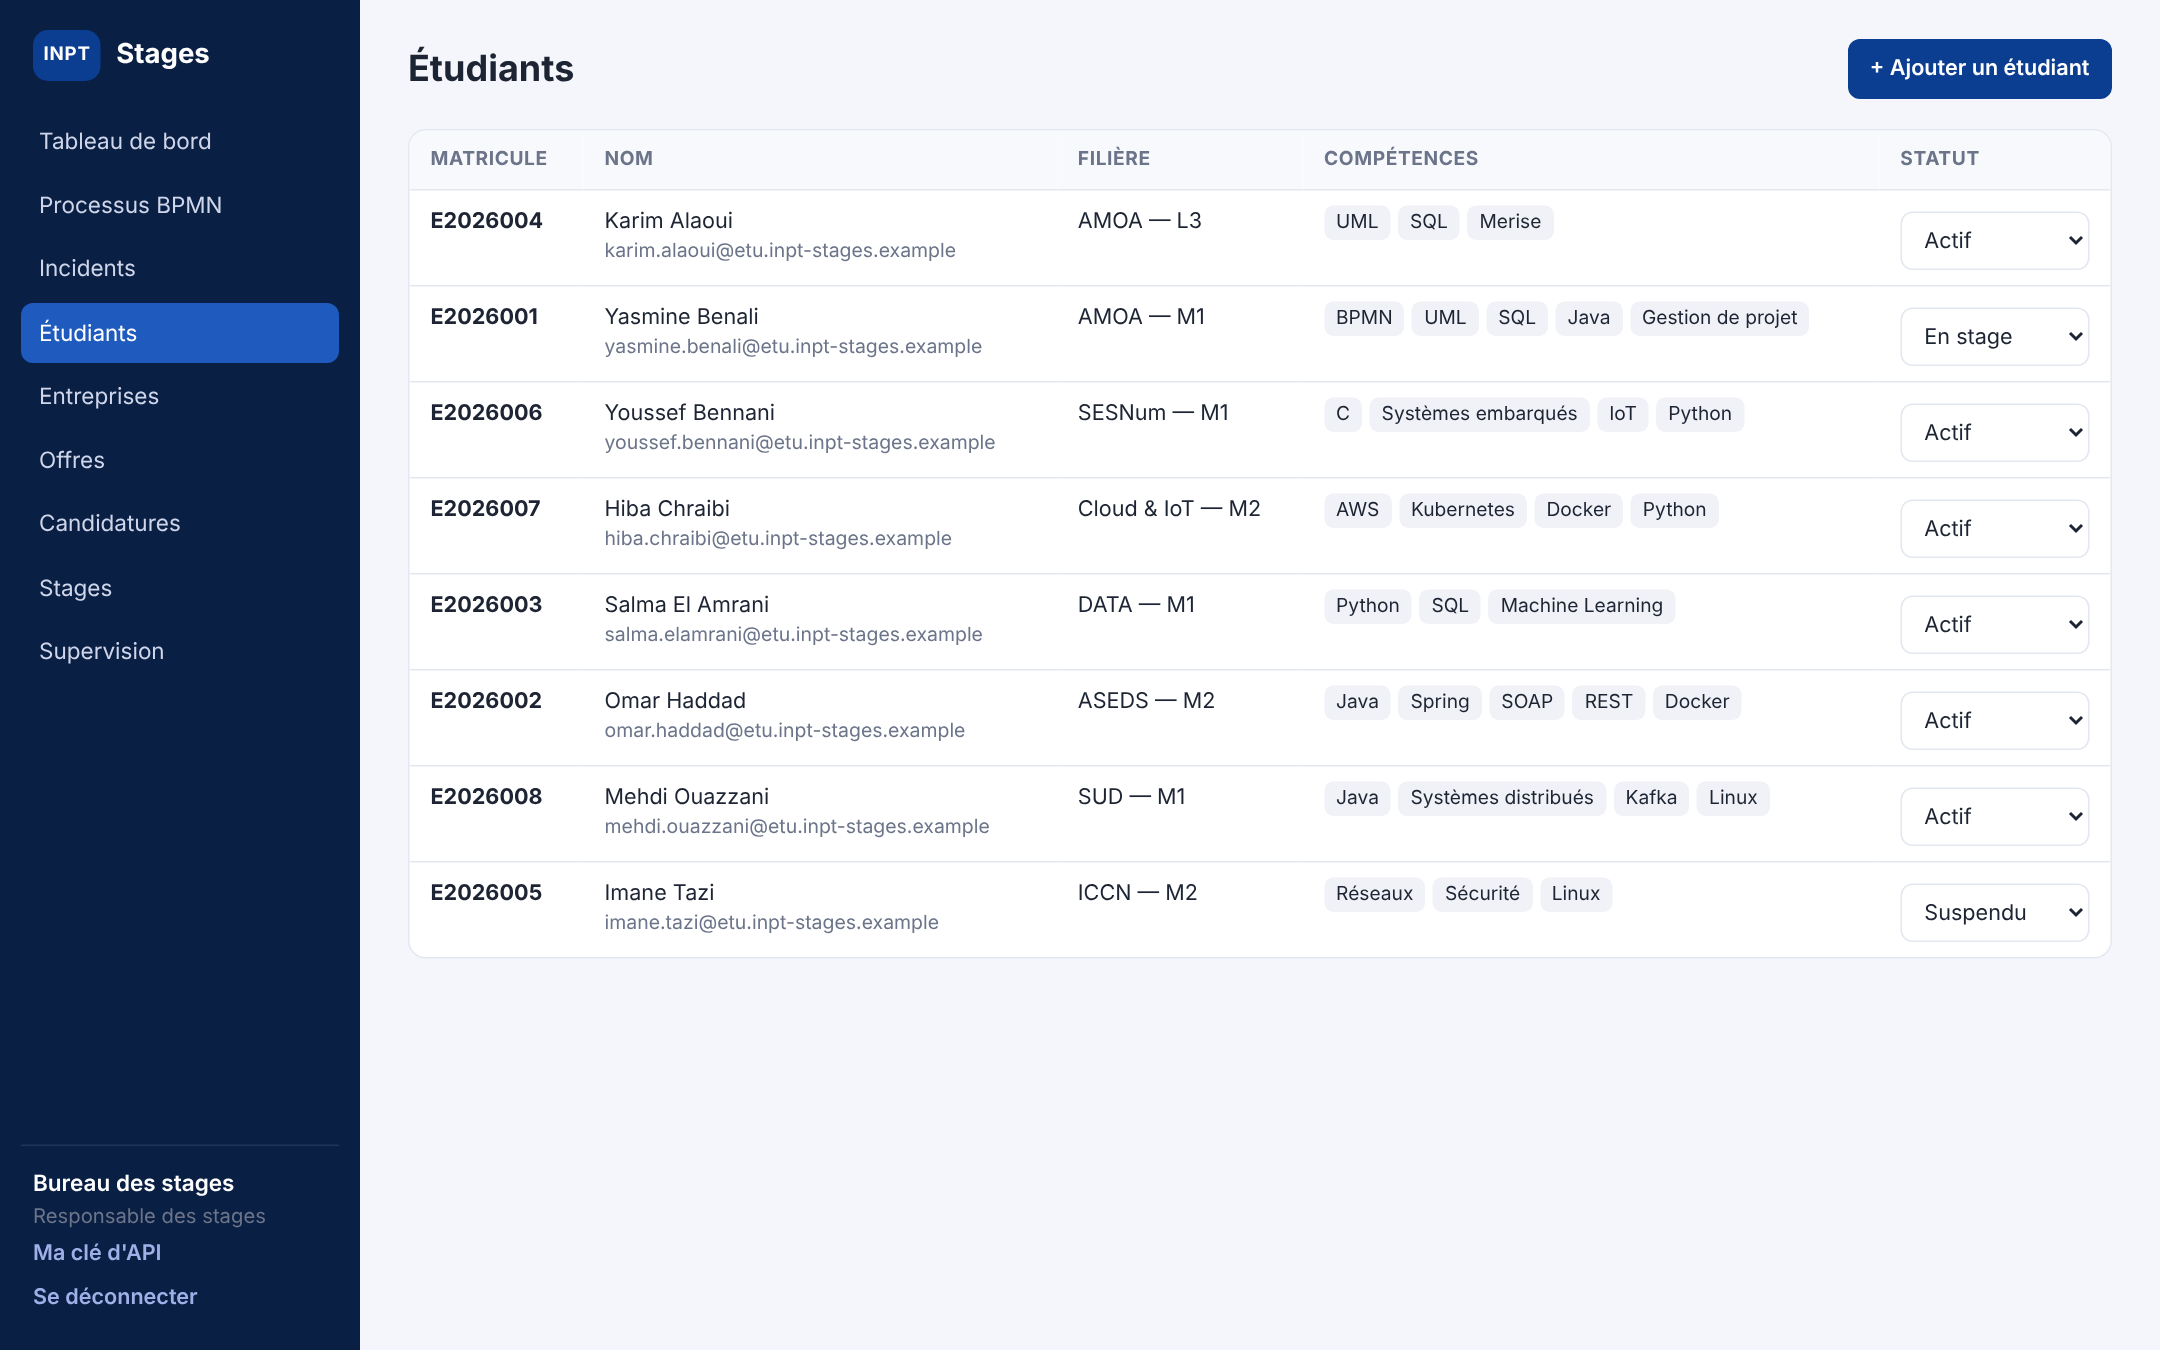
\includegraphics[width=\linewidth]{figures/ui-admin-etudiants.png}\\[-2pt]{\small (b) gestion des étudiants (SOAP)}
\end{minipage}
\caption{Écrans d'administration}
\end{figure}

\chapter{Bilan et perspectives}\label{chap:conclusion}

\section{Bilan}
Le projet livre une plateforme complète et opérationnelle : six services autonomes aux contrats explicites,
trois en SOAP décrits par WSDL et trois en REST, orchestrés par un processus BPMN 2.0 réellement exécuté.
Le processus couvre les neuf étapes demandées et va au-delà sur trois points : demande de complément d'information,
relance automatique de l'entreprise et interruption sur annulation. La gestion des erreurs combine reprise
automatique, événements d'erreur BPMN et traitement humain des incidents, avec des reprises idempotentes.
L'ensemble est vérifié par 28 tests d'intégration de bout en bout, sur H2 et PostgreSQL, et peut être utilisé par
chaque acteur à travers l'interface web.

\section{Limites}
\begin{itemize}
  \item Les six services partagent un processus et une base physique pour simplifier la démonstration ; l'isolation
        est logique (tables, contrats, appels réseau), pas physique.
  \item Le transport n'est pas chiffré dans l'environnement de démonstration (HTTPS à activer en production).
\end{itemize}

\section{Perspectives}
\begin{itemize}
  \item Déployer chaque service dans son propre conteneur avec sa base (Docker Compose ou Kubernetes) et un annuaire
        de services ou une passerelle d'API.
  \item Remplacer HTTP Basic par des jetons OAuth 2 / JWT, et signer les messages SOAP (WS-Security \emph{Signature}).
  \item Ajouter un disjoncteur (\emph{circuit breaker}) et une file de messages pour les notifications.
  \item Remplacer Mailpit par le serveur SMTP de l'école et ajouter des notifications instantanées dans l'application.
  \item Enrichir la compatibilité par une recommandation d'offres fondée sur l'historique des stages.
\end{itemize}


\appendix
\chapter{Mise en œuvre}

\section{Lancement}
\begin{lstlisting}[language=sh]
mailpit                            # boîte e-mail de test : http://localhost:8025 (SMTP 1025)
mvn package                        # compile, teste (31 tests) et produit le jar
java -jar target/gestion-stages.jar
# Interface : http://localhost:8090/       WSDL : http://localhost:8090/ws/etudiants?wsdl

docker compose up --build          # variante tout-en-un : plateforme + PostgreSQL + Mailpit
cd rapport && latexmk -pdf rapport.tex
\end{lstlisting}

\section{Comptes de démonstration}\label{annexe:comptes}
\begin{table}[htbp]
\centering\small
\caption{Comptes de démonstration}
\begin{tabularx}{\textwidth}{@{}llY@{}}
\toprule
\textbf{Identifiant} & \textbf{Mot de passe} & \textbf{Profil} \\
\midrule
\code{admin} & \code{Admin@2026} & Responsable des stages \\
\code{E2026001} & \code{Etudiant@2026} & Yasmine Benali — AMOA, INE2 \\
\code{E2026002} & \code{Etudiant@2026} & Omar Haddad — ASEDS, INE3 \\
\code{E2026003} & \code{Etudiant@2026} & Salma El Amrani — DATA, INE2 \\
\code{E2026004} & \code{Etudiant@2026} & Karim Alaoui — AMOA, INE1 \\
\code{E2026005} & \code{Etudiant@2026} & Imane Tazi — ICCN, INE3, \emph{suspendue} \\
\code{E2026006} à \code{E2026008} & \code{Etudiant@2026} & Youssef Bennani (SESNum), Hiba Chraibi (Cloud \& IoT), Mehdi Ouazzani (SUD) \\
\code{atlas}, \code{nova}, \code{fintech}, \code{cyber}, \code{cloud} & \code{Entreprise@2026} & Entreprises référencées \\
\code{startup} & \code{Entreprise@2026} & Entreprise non référencée \\
\code{systeme} & \code{Systeme@2026} & Compte technique de l'orchestrateur \\
\bottomrule
\end{tabularx}
\end{table}

Chaque compte dispose d'une clé d'API de démonstration \code{stg\_demo\_<identifiant>} (par exemple
\code{stg\_demo\_admin}), utilisable dans l'en-tête \code{X-API-Key} des appels REST.

\section{Organisation du code source}
\begin{lstlisting}
src/main/java/com/universite/stages/
  soap/etudiants|entreprises|offres     services 1 à 3 : contrat, implémentation, DAO, DTO JAXB
  rest/candidatures|notifications|stages services 4 à 6 : ressources JAX-RS, DAO
  rest/processus                        API d'orchestration
  bpmn/                                 moteur Flowable et délégués des tâches de service
  clients/                              clients SOAP dynamiques, client REST, politique de reprise
  security/                             WS-Security, PBKDF2, rôles
  common/                               configuration, JDBC, validation, simulateur de pannes
src/main/resources/
  processes/candidature-stage.bpmn20.xml  processus BPMN 2.0 (modèle + diagramme)
  schema.sql  application.properties  public/ (interface web)
src/test/java/.../PlateformeIT.java     24 tests d'intégration
docs/  wsdl/  soap/  postman/  SCENARIO_VIDEO.md
tools/ generer_bpmn.py  rendre_bpmn.js  captures_ui.js
\end{lstlisting}


\end{document}
